\documentclass[]{elsarticle} %review=doublespace preprint=single 5p=2 column
%%% Begin My package additions %%%%%%%%%%%%%%%%%%%

\usepackage[hyphens]{url}

  \journal{Some Journal} % Sets Journal name

\usepackage{lineno} % add
  \linenumbers % turns line numbering on

\usepackage{graphicx}
%%%%%%%%%%%%%%%% end my additions to header

\usepackage[T1]{fontenc}
\usepackage{lmodern}
\usepackage{amssymb,amsmath}
\usepackage{ifxetex,ifluatex}
\usepackage{fixltx2e} % provides \textsubscript
% use upquote if available, for straight quotes in verbatim environments
\IfFileExists{upquote.sty}{\usepackage{upquote}}{}
\ifnum 0\ifxetex 1\fi\ifluatex 1\fi=0 % if pdftex
  \usepackage[utf8]{inputenc}
\else % if luatex or xelatex
  \usepackage{fontspec}
  \ifxetex
    \usepackage{xltxtra,xunicode}
  \fi
  \defaultfontfeatures{Mapping=tex-text,Scale=MatchLowercase}
  \newcommand{\euro}{€}
\fi
% use microtype if available
\IfFileExists{microtype.sty}{\usepackage{microtype}}{}
\usepackage[]{natbib}
\bibliographystyle{plainnat}

\ifxetex
  \usepackage[setpagesize=false, % page size defined by xetex
              unicode=false, % unicode breaks when used with xetex
              xetex]{hyperref}
\else
  \usepackage[unicode=true]{hyperref}
\fi
\hypersetup{breaklinks=true,
            bookmarks=true,
            pdfauthor={},
            pdftitle={Introducing spatial availability, a singly-constrained measure of competitive accessibility},
            colorlinks=false,
            urlcolor=blue,
            linkcolor=magenta,
            pdfborder={0 0 0}}

\setcounter{secnumdepth}{5}
% Pandoc toggle for numbering sections (defaults to be off)


% tightlist command for lists without linebreak
\providecommand{\tightlist}{%
  \setlength{\itemsep}{0pt}\setlength{\parskip}{0pt}}



\usepackage[font=small,skip=0pt]{caption}
\usepackage{booktabs}
\usepackage{longtable}
\usepackage{array}
\usepackage{multirow}
\usepackage{wrapfig}
\usepackage{float}
\usepackage{colortbl}
\usepackage{pdflscape}
\usepackage{tabu}
\usepackage{threeparttable}
\usepackage{threeparttablex}
\usepackage[normalem]{ulem}
\usepackage{makecell}
\usepackage{xcolor}
\usepackage{caption}
\usepackage{graphicx}
\usepackage{siunitx}
\usepackage{hhline}
\usepackage{calc}
\usepackage{tabularx}
\usepackage{adjustbox}
\usepackage{hyperref}



\begin{document}


\begin{frontmatter}

  \title{Introducing spatial availability, a singly-constrained measure
of competitive accessibility}
      \cortext[cor1]{Corresponding author}
  
  \begin{abstract}
  Accessibility indicators are widely used in transportation, urban, and
  healthcare planning, among many other applications. These measures are
  weighted sums of reachable opportunities from a given origin
  conditional on the cost of movement, and are estimates of the
  potential for spatial interaction. Over time, various proposals have
  been forwarded to improve their interpretability, mainly by
  introducing competition. In this paper, we demonstrate how a widely
  used measure of accessibility with congestion fails to properly match
  the opportunity-seeking population. We then propose an alternative
  formulation of accessibility with competition, a measure we call
  \emph{spatial availability}. This measure results from using balancing
  factors that are equivalent to imposing a single constraint on
  conventional gravity-based accessibility. Further, we demonstrate how
  Two-Stage Floating Catchment Area (2SFCA) methods can be
  reconceptualized as singly-constrained accessibility. To illustrate
  the application of spatial availability and compare it to other
  relevant measures, we use data from the 2016 Transportation Tomorrow
  Survey of the Greater Golden Horseshoe area in southern Ontario,
  Canada.
  \end{abstract}
  
 \end{frontmatter}

\newpage

\hypertarget{sec:introduction}{%
\section{Introduction}\label{sec:introduction}}

The concept of accessibility in transportation studies derives its
appeal from the combination of the spatial distribution of opportunities
and the cost of reaching them \citep{hansen1959, handy_measuring_1997}.
Accessibility analysis is employed in transportation, geography, public
health, and many other areas, with the number of applications growing
\citep{shi_literature_2020}, especially as mobility-based planning is
de-emphasized in favor of access-oriented planning
\citep{deboosere2018, handy2020, proffitt2017, yan2021}.

Accessibility analysis stems from the foundational works of
\citet{harris_market_1954} and \citet{hansen1959}. From these seminal
efforts, many accessibility measures have been derived, particularly
after the influential work of \citet{wilson1971} on spatial
interaction\footnote{Utility-based measures derive from a very different
  theoretical framework, random utility maximization}. Of these,
gravity-type accessibility is arguably the most common; since its
introduction in the literature, it has been widely adopted in numerous
forms
\citep{cervero_transportation_2002, paez2004network, geurs2004, levinson_accessibility_1998, Arranz2019measuring}.
Hanson-type accessibility indicators are essentially weighted sums of
opportunities, with the weights given by an impedance function that
depends on the cost of movement, and thus measure the \emph{intensity of
the possibility of interaction} \citep{hansen1959}. This type of
accessibility analysis offers a powerful tool to study the intersection
between urban structure and transportation infrastructure
\citep{handy_measuring_1997}.

Despite their usefulness, the interpretability of Hansen-type
accessibility measures can be challenging \citep{geurs2004, miller2018}.
Since they aggregate opportunities, the results are sensitive to the
size of the region of interest (e.g., a large city has more jobs than a
smaller city). As a consequence, raw outputs are not necessarily
comparable across study areas \citep{allen2019}. This limitation becomes
evident when surveying studies that implement this type of analysis. For
example, \citet{paez_healthcare_2010} (in Montreal) and
\citet{campbell_2019_accessibility} (in Nairobi) report accessibility as
the number of health care facilities that can potentially be reached
from origins. But what does it mean for a zone to have accessibility to
less than 100 facilities in each of these two cities, with their
different populations and number of facilities? For that matter, what
does it mean for a zone to have accessibility to more than 700
facilities in Montreal, besides being ``accessibility rich''? As another
example, \citet{bocarejo_s_transport_2012} (in Bogota),
\citet{elgeneidy_cost_2016} (in Montreal), and
\citet{jiang_2016_accessibility} (in Beijing) report accessibility as
numbers of jobs, with accessibility values often in the hundreds of
thousands, and even exceeding one million jobs for some zones in Beijing
and Montreal. As indicators of urban structure, these measures are
informative, but the meaning of one million accessible jobs is harder to
pin down: how many jobs must any single person have access to? Clearly,
the answer to this question depends on how many people demand jobs.

The interpretability of Hansen-type accessibility has been discussed in
numerous studies, including recently by \citet{hu_2019_measuring},
\citet{kelobonye2020measuring}, and in greater depth by
\citet{merlin2017competition}. As hinted above, the limitations in
interpretability are frequently caused by ignoring competition - without
competition, each opportunity is assumed to be equally available to
every single opportunity-seeking individual that can reach it
\citep{shen1998, paez2019, kelobonye2020measuring}. This assumption is
appropriate when the opportunity of interest is non-exclusive, that is,
if use by one unit of population does not preclude use by another. For
instance, national parks with abundant space are seldom used to full
capacity, so the presence of some population does not exclude use by
others. When it comes to exclusive opportunities, or when operations may
be affected by congestion, the solution has been to account for
competition. Several efforts exist that do so. In our reckoning, the
first such approach was proposed by \citet{weibull_axiomatic_1976},
whereby the distance decay of the supply of employment and the demand
for employment (by workers) were formulated under so-called axiomatic
assumptions. This approach was then applied by \citet{joseph1984} in the
context of healthcare, to quantify the availability of general
practitioners in Canada. About two decades later, \citet{shen1998}
independently re-discovered Weibull's
\citeyearpar{weibull_axiomatic_1976} formula \citep[see footnote (7)
in][]{shen1998} and deconstructed it to consider accessibility for
different modes. These advances were subsequently popularized as the
family of Two-Stage Floating Catchment area (2SFCA) methods
\citep{luo2003} that have found widespread adoption in healthcare,
education, and food systems
\citep{yang_comparing_2006, chen_spatial_2020, ye_spatial_2018, chen_enhancing_2019, chen_evaluating_2020}.

An important development contained in Shen's work is a proof that the
population-weighted sum of the accessibility measure with competition
equates to the number of opportunities available \citep[footnote (7) and
Appendix A in][]{shen1998}. This demonstration gives the impression that
Shen-type accessibility allocates \emph{all} opportunities to the
origins, however to the authors' knowledge, it has not interpreted by
literature in this way. For instance, \citet{hu_changing_2014},
\citet{merlin2017competition}, and \citet{tao_investigating_2020} all
use Shen-type accessibility to calculate job access but report values as
`competitive accessibility scores' or simply `job accessibility'. These
works do not explicitly recognize that jobs that are assigned to each
origin are in fact a proportion of \emph{all} the opportunities in the
system. This recognition, we argue, is critical to interpreting the
meaning of the final result. Thus, in this paper we intend to revisit
accessibility with competition within the context of disentangling how
opportunities are allocated. We first argue that Shen's competitive
accessibility misleadingly refers to the the total zonal population to
equal the travel-cost discounted opportunity-seeking population. This
equivocation, we believe, results in a ambigious interpretation of what
Shen-type accessibility represents as the allocation of opportunities to
population is masked by the results presenting as rates (i.e.,
opportunities per capita). We then propose an alternative formulation of
accessibility that incorporates competition by adopting a proportional
allocation mechanism; we name this measure \emph{spatial availability}.
The use of balancing factors for proportional allocation is akin to
imposing a single constraint on the accessibility indicator, in the
spirit of Wilson's \citeyearpar{wilson1971} spatial interaction model.

In this way, the aim of the paper is three-fold:

\begin{itemize}
\item
  First, we aim to demonstrate that Shen-type (and thus
  \citet{weibull_axiomatic_1976} accessibility and the popular 2SFCA
  methods) produce equivocal estimates of opportunities allocated as the
  result is presented as a rate (i.e., opportunities per capita);
\item
  Second, we introduce a new measure, \emph{spatial availability}, which
  we submit is a more interpretable alternative to Shen-type
  accessibility, since opportunities in the system are preserved and
  proportionally allocated to the population; and
\item
  Third, we show how Shen-type accessibility (and 2SFCA methods) can be
  seen as measures of singly-constrained accessibility.
\end{itemize}

Discussion is supported by the use of the small synthetic example of
\citet{shen1998} and empirical data drawn from the 2016 Transportation
Tomorrow Survey of the Greater Toronto and Hamilton Area in Ontario,
Canada. In the spirit of openness of research in the spatial sciences
\citep{brunsdon2021opening, paez2021open} this paper has a companion
open data product \citep{arribas2021Open}, and all code is available for
replicability and reproducibility purposes at
\url{https://github.com/soukhova/Spatial-Availability-Measure}.

\hypertarget{background}{%
\section{Accessibility measures revisited}\label{background}}

In this section we revisit Hansen-type and Shen-type accessibility
indicators. We adopt the convention of using a capital letter for
absolute values (number of opportunities) and lower case for rates
(opportunities per capita).

\hypertarget{hansen-type-accessibility}{%
\subsection{Hansen-type accessibility}\label{hansen-type-accessibility}}

Hansen-type accessibility measures follow the general formulation shown
in Equation (\ref{eq:conventional-accessibility}):

\begin{equation}
\label{eq:conventional-accessibility}
S_i = \sum_{j=1}^JO_j \cdot f(c_{ij})
\end{equation}

\noindent where:

\begin{itemize}
\tightlist
\item
  \(c_{ij}\) is a measure of the cost of moving between \(i\) and \(j\).
\item
  \(f(\cdot)\) is an impedance function of \(c_{ij}\); it can take the
  form of any monotonically decreasing function chosen based on positive
  or normative criteria \citep{paez2012measuring}.
\item
  \(i\) is a set of origin locations (\(i = 1,\cdots,N\)).
\item
  \(j\) is a set of destination locations (\(j = 1,\cdots,J\)).
\item
  \(O_j\) is the number of opportunities at location \(j\);
  \(O = \sum_{j=1}^J O_j\) is the total supply of opportunities in the
  study region.
\item
  \(S\) is Hansen-type accessibility as weighted sum of opportunities.
\end{itemize}

As formally defined, accessibility \(S_i\) is the sum of opportunities
that can be reached from location \(i\), weighted down by an impedance
function of the cost of travel \(c_{ij}\). Summing the opportunities in
the neighborhood of \(i\) provides estimates of the number of
opportunities that can \emph{potentially} be reached from \(i\). Several
measures result from using a variety of impedance functions; for
example, cumulative opportunities measures are obtained when
\(f(\cdot)\) is a binary or indicator function
\citep[e.g.,][]{elgeneidy_cost_2016, rosik_forecast_2021, geurs2004, qi_decadelong_2018}.
Other measures use impedance functions modeled after any monotonically
decreasing function \citep[e.g., Gaussian, inverse power, negative
exponential, or log-normal, among others, see, \emph{inter
alia},][]{kwan_spacetime_1998, vale_influence_2017, reggiani_accessibility_2011, li_approach_2020}.
In practice, accessibility measures with different impedance functions
tend to be highly correlated
\citep{higgins2019, santanapalacios2022, kwan_spacetime_1998}.

Gravity-based accessibility has been shown to be an excellent indicator
of the intersection between spatially distributed opportunities and
transportation infrastructure
\citep{shi_literature_2020, reggiani_accessibility_2011, kwan_spacetime_1998}.
However, beyond enabling comparisons of relative values they are not
highly interpretable on their own \citep{miller2018}. To address the
issue of interpretability, previous research has aimed to index and
normalize values on a per demand-population basis
\citep[e.g.,][]{barboza_balancing_2021, pereira_distributional_2019, wang_access_2021}.
However, as recent research on accessibility discusses
\citep[e.g.,][]{merlin2017competition, allen2019, paez2019, kelobonye2020measuring},
these steps do not adequately consider competition. In effect, when
calculating \(S_i\), every opportunity enters the weighted sum once for
every origin \(i\) that can reach it. This makes interpretability
opaque, and to complicate matters, can also bias the estimated landscape
of opportunity.

\hypertarget{shen-type-competitive-accessibility}{%
\subsection{Shen-type competitive
accessibility}\label{shen-type-competitive-accessibility}}

To account for competition, the influential works of \citet{shen1998}
and \citet{weibull_axiomatic_1976}, as well as the widely used 2SFCA
approach of \citet{luo2003}, adjust Hansen-type accessibility with the
population in the region of interest. The mechanics of this approach
consist of calculating, for every destination \(j\), the population that
can reach it given the impedance function \(f(\cdot)\); let us call this
the \emph{effective opportunity-seeking population} (Equation
(\ref{eq:effective-opportunity-seeking-population})). This value can be
seen as the Hansen-type \emph{market area} (accessibility to population)
of \(j\). The opportunities at \(j\) are then divided by the sum of the
effective opportunity-seeking population to obtain a measure of
opportunities per capita, i.e., \(R_j\) in Equation
(\ref{eq:level-of-service}). This can be thought of as the \emph{level
of service} at \(j\). Per capita values are then allocated back to the
population at \(i\), again subject to the impedance function as seen in
Equation (\ref{eq:2SFCA-step2}); this is accessibility with competition.

\begin{equation}
\label{eq:effective-opportunity-seeking-population}
P_{ij}^* = P_{i} \cdot f(c_{ij})\\
\end{equation}

\begin{equation}
\label{eq:level-of-service}
R_{j} = \frac{O_{j}}{\sum_i P_{ij}^*}\\
\end{equation}

\begin{equation}
\label{eq:2SFCA-step2}
a_{i} = {\sum_j R_{j} \cdot f(c_{ij})}\\
\end{equation}

\noindent where:

\begin{itemize}
\tightlist
\item
  \(a\) is Shen-type accessibility as weighted sum of opportunities per
  capita (or weighted level of service).
\item
  \(c_{ij}\) is a measure of the cost of moving between \(i\) and \(j\).
\item
  \(f(\cdot)\) is an impedance function of \(c_{ij}\).
\item
  \(i\) is a set of origin locations (\(i = 1,\cdots,N\)).
\item
  \(j\) is a set of destination locations (\(j = 1,\cdots,J\)).
\item
  \(O_j\) is the number of opportunities at location \(j\);
  \(O = \sum_{j=1}^J O_j\) is the total supply of opportunities in the
  study region.
\item
  \(P_i\) is the population at location \(i\).
\item
  \(P_{ij}^*\) is the population at location \(i\) that can reach
  destination \(j\) according to the impedance function; we call this
  the \emph{effective opportunity-seeking population}.
\item
  \(R_j\) is the ratio of opportunities at \(j\) to the sum over all
  origins of the \emph{effective opportunity-seeking population} that
  can reach \(j\); in other words, this is the total number of
  opportunities per capita found at \(j\).
\end{itemize}

\citet{shen1998} describes \(P_i\) as the \emph{``the number of people
in location \(i\) seeking opportunities''}. In our view, this is
somewhat equivocal and where misinterpretation of the final results may
arise. Consider a population center where the population is only willing
to take an opportunity if the trip required is less than or equal to 60
minutes. This is identical to the following impedance function:

\begin{equation}
\label{eq:binary-impedance}
f(c_{ij}) =
\begin{cases}
1\text{ if }c_{ij}\leq60\text{ min}\\
0\text{ otherwise}\\
\end{cases}
\end{equation}

If an employment center is less than 60 minutes away, the population can
seek opportunities there (i.e., \(f(c_{ij})=1\)). But are these people
still part of the opportunity-seeking population for jobs located two
hours away? Four hours? Ten hours? We assume that they are not because
their travel behaviour, as represented by the impedance function would
yield \(f(c_{ij})=0\), eliminating them from the effective
opportunity-seeking population \(P_ij*\). We see Shen's definition as
ambiguous because, for the purpose of calculating accessibility, the
impedance function defines what constitutes the population that
effectively can seek opportunities at remote locations. Thus \(P_i\)
should be plainly understood as the population at location \(i\) (as
defined above) and not the \emph{``the number of people in location
\(i\) seeking opportunities''}. In other words, \(P_i\) and \(P_{ij}*\)
are confounded.

Furthermore, an identical misunderstanding can be described for \(O_j\)
which is defined as \emph{``the number of \textbf{relevant}
opportunities in location j''} in \citet{shen1998} (our emphasis).
\(O_j\) is adjusted by the same \(f(c_{ij})\) in Equation
(\ref{eq:2SFCA-step2}), so the \emph{relevancy} is determined by the
travel behaviour associated with the impedance function not purely by
\(O_j\) itself. For this reason, \(O_j\) should be understand plainly as
the opportunities at location \(j\) (as we also defined them above).

Misunderstanding \(P_i\) and \(O_j\) may lead to a misleading
interpretation of the final result \(a_i\), especially as expressed in
Shen's proof (see Equation (\ref{eq:2SFCA-total})).

\begin{equation}
\label{eq:2SFCA-total}
\sum_{i=1}^N a_{i} P_i= \sum_{j=1}^JO_j\\
\end{equation}

Notice, confounding \(P_i\) and \(O_j\) with the effective
opportunity-seeking population and the jobs they take may cause us to
misunderstand \(a_{i}\) as \emph{``relevant opportunities''} per
\emph{``people in location \(i\) seeking opportunities''}. Instead, as
mathematically expressed in the proof, \(a_{i}\) is a proportion of the
opportunities available to the population, since multiplying \(a_i\) by
the population at \(i\) and summing for all origins in the system equals
to the total number of opportunities in the system. Embedded in \(a_i\)
is already the travel behaviour so \(P_i\) and \(O_j\) must be plainly
understand as population at \(i\) and opportunities at \(j\) to have
Equation (\ref{eq:2SFCA-total}) hold true.

\hypertarget{shens-synthetic-example}{%
\subsection{Shen's synthetic example}\label{shens-synthetic-example}}

In this section we use the example in \citet{shen1998} to detail the
importance of understanding \(P_i\) and \(O_j\) as simply the population
at the origin \(i\) and the opportunities at destination \(j\)
respectively. This is critical to understanding how the opportunities
are allocated to the population based on the impedance function.

\begin{figure}

{\centering 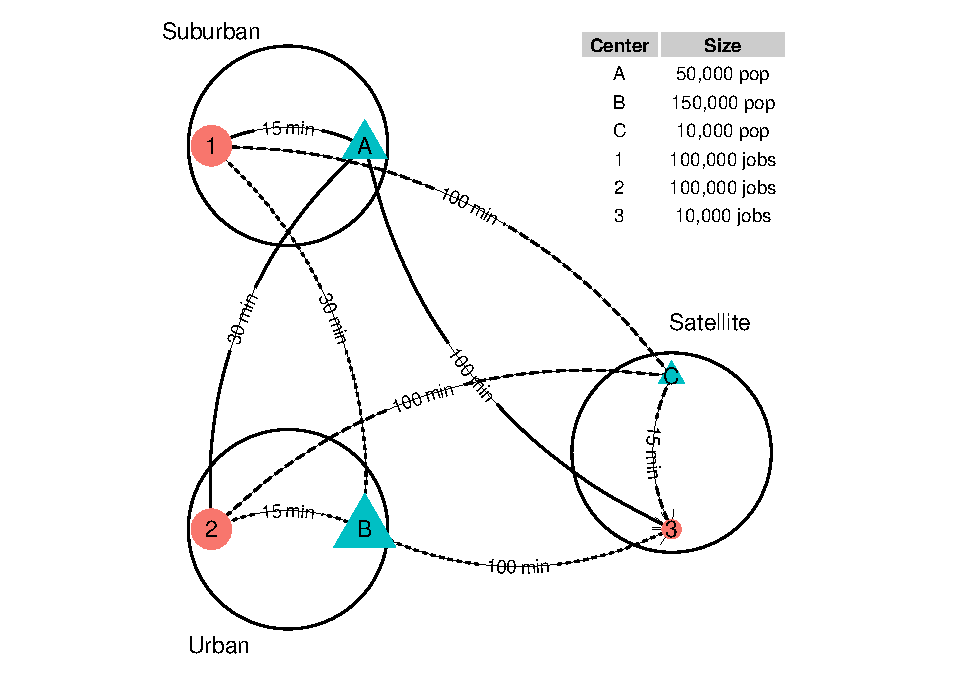
\includegraphics[width=1\linewidth]{Spatial-Availability-Refreshed_files/figure-latex/create-figure-with-toy-example-1} 

}

\caption{\label{fig:plot-toy-example} Shen (1998) synthetic example with locations of employment centers (in orange), population centers (in blue), number of jobs and population, and travel times.}\label{fig:create-figure-with-toy-example}
\end{figure}

 
  \providecommand{\huxb}[2]{\arrayrulecolor[RGB]{#1}\global\arrayrulewidth=#2pt}
  \providecommand{\huxvb}[2]{\color[RGB]{#1}\vrule width #2pt}
  \providecommand{\huxtpad}[1]{\rule{0pt}{#1}}
  \providecommand{\huxbpad}[1]{\rule[-#1]{0pt}{#1}}

\begin{table}[ht]
\begin{centerbox}
\begin{threeparttable}
\captionsetup{justification=centering,singlelinecheck=off}
\caption{Summary description of synthetic example: Hansen-type accessibility and Shen-type accessibility with competition with beta = 0.1}
 \label{tab:synthetic-example}
\setlength{\tabcolsep}{0pt}
\begin{tabularx}{1.2\textwidth}{p{0.12\textwidth} p{0.12\textwidth} p{0.12\textwidth} p{0.12\textwidth} p{0.12\textwidth} p{0.12\textwidth} p{0.12\textwidth} p{0.12\textwidth} p{0.12\textwidth} p{0.12\textwidth}}


\hhline{>{\huxb{190, 190, 190}{1}}|>{\huxb{190, 190, 190}{1}}|>{\huxb{190, 190, 190}{1}}|>{\huxb{190, 190, 190}{1}}|>{\huxb{190, 190, 190}{1}}|>{\huxb{190, 190, 190}{1}}|>{\huxb{190, 190, 190}{1}}|>{\huxb{190, 190, 190}{1}}|>{\huxb{190, 190, 190}{1}}|}
\arrayrulecolor{black}

\multicolumn{1}{!{\huxvb{0, 0, 0}{0}}p{0.12\textwidth}!{\huxvb{190, 190, 190}{1}}}{\hspace{6pt}\parbox[b]{0.12\textwidth-6pt-6pt}{\huxtpad{6pt + 1em}\raggedright \textbf{{\fontsize{7pt}{8.4pt}\selectfont Origin}}\huxbpad{6pt}}} &
\multicolumn{1}{p{0.12\textwidth}!{\huxvb{190, 190, 190}{1}}}{\hspace{6pt}\parbox[b]{0.12\textwidth-6pt-6pt}{\huxtpad{6pt + 1em}\centering \textbf{{\fontsize{7pt}{8.4pt}\selectfont Pop.}}\huxbpad{6pt}}} &
\multicolumn{1}{p{0.12\textwidth}!{\huxvb{190, 190, 190}{1}}}{\hspace{6pt}\parbox[b]{0.12\textwidth-6pt-6pt}{\huxtpad{6pt + 1em}\raggedright \textbf{{\fontsize{7pt}{8.4pt}\selectfont Dest.}}\huxbpad{6pt}}} &
\multicolumn{1}{p{0.12\textwidth}!{\huxvb{190, 190, 190}{1}}}{\hspace{6pt}\parbox[b]{0.12\textwidth-6pt-6pt}{\huxtpad{6pt + 1em}\centering \textbf{{\fontsize{7pt}{8.4pt}\selectfont Jobs}}\huxbpad{6pt}}} &
\multicolumn{1}{p{0.12\textwidth}!{\huxvb{190, 190, 190}{1}}}{\hspace{6pt}\parbox[b]{0.12\textwidth-6pt-6pt}{\huxtpad{6pt + 1em}\centering \textbf{{\fontsize{7pt}{8.4pt}\selectfont TT}}\huxbpad{6pt}}} &
\multicolumn{1}{p{0.12\textwidth}!{\huxvb{190, 190, 190}{1}}}{\hspace{6pt}\parbox[b]{0.12\textwidth-6pt-6pt}{\huxtpad{6pt + 1em}\centering \textbf{{\fontsize{7pt}{8.4pt}\selectfont f(TT)}}\huxbpad{6pt}}} &
\multicolumn{1}{p{0.12\textwidth}!{\huxvb{190, 190, 190}{1}}}{\hspace{6pt}\parbox[b]{0.12\textwidth-6pt-6pt}{\huxtpad{6pt + 1em}\centering \textbf{{\fontsize{7pt}{8.4pt}\selectfont Pop * f(TT)}}\huxbpad{6pt}}} &
\multicolumn{1}{p{0.12\textwidth}!{\huxvb{190, 190, 190}{1}}}{\hspace{6pt}\parbox[b]{0.12\textwidth-6pt-6pt}{\huxtpad{6pt + 1em}\centering \textbf{{\fontsize{7pt}{8.4pt}\selectfont Jobs * f(TT)}}\huxbpad{6pt}}} &
\multicolumn{1}{p{0.12\textwidth}!{\huxvb{190, 190, 190}{1}}}{\hspace{6pt}\parbox[b]{0.12\textwidth-6pt-6pt}{\huxtpad{6pt + 1em}\centering \textbf{{\fontsize{7pt}{8.4pt}\selectfont S\_i}}\huxbpad{6pt}}} &
\multicolumn{1}{p{0.12\textwidth}!{\huxvb{0, 0, 0}{0}}}{\hspace{6pt}\parbox[b]{0.12\textwidth-6pt-6pt}{\huxtpad{6pt + 1em}\centering \textbf{{\fontsize{7pt}{8.4pt}\selectfont a\_i}}\huxbpad{6pt}}} \tabularnewline[-0.5pt]


\hhline{>{\huxb{0, 0, 0}{0.4}}->{\huxb{0, 0, 0}{0.4}}->{\huxb{0, 0, 0}{0.4}}->{\huxb{0, 0, 0}{0.4}}->{\huxb{0, 0, 0}{0.4}}->{\huxb{0, 0, 0}{0.4}}->{\huxb{0, 0, 0}{0.4}}->{\huxb{0, 0, 0}{0.4}}->{\huxb{0, 0, 0}{0.4}}->{\huxb{0, 0, 0}{0.4}}-}
\arrayrulecolor{black}

\multicolumn{1}{!{\huxvb{0, 0, 0}{0}}p{0.12\textwidth}!{\huxvb{190, 190, 190}{1}}}{} &
\multicolumn{1}{p{0.12\textwidth}!{\huxvb{190, 190, 190}{1}}}{} &
\multicolumn{1}{p{0.12\textwidth}!{\huxvb{190, 190, 190}{1}}}{\hspace{6pt}\parbox[b]{0.12\textwidth-6pt-6pt}{\huxtpad{6pt + 1em}\raggedright {\fontsize{7pt}{8.4pt}\selectfont 1}\huxbpad{6pt}}} &
\multicolumn{1}{p{0.12\textwidth}!{\huxvb{190, 190, 190}{1}}}{\hspace{6pt}\parbox[b]{0.12\textwidth-6pt-6pt}{\huxtpad{6pt + 1em}\centering {\fontsize{7pt}{8.4pt}\selectfont 100,000}\huxbpad{6pt}}} &
\multicolumn{1}{p{0.12\textwidth}!{\huxvb{190, 190, 190}{1}}}{\hspace{6pt}\parbox[b]{0.12\textwidth-6pt-6pt}{\huxtpad{6pt + 1em}\centering {\fontsize{7pt}{8.4pt}\selectfont 15}\huxbpad{6pt}}} &
\multicolumn{1}{p{0.12\textwidth}!{\huxvb{190, 190, 190}{1}}}{\hspace{6pt}\parbox[b]{0.12\textwidth-6pt-6pt}{\huxtpad{6pt + 1em}\centering {\fontsize{7pt}{8.4pt}\selectfont 0.223130}\huxbpad{6pt}}} &
\multicolumn{1}{p{0.12\textwidth}!{\huxvb{190, 190, 190}{1}}}{\hspace{6pt}\parbox[b]{0.12\textwidth-6pt-6pt}{\huxtpad{6pt + 1em}\centering {\fontsize{7pt}{8.4pt}\selectfont 11,157}\huxbpad{6pt}}} &
\multicolumn{1}{p{0.12\textwidth}!{\huxvb{190, 190, 190}{1}}}{\hspace{6pt}\parbox[b]{0.12\textwidth-6pt-6pt}{\huxtpad{6pt + 1em}\centering {\fontsize{7pt}{8.4pt}\selectfont 22,313}\huxbpad{6pt}}} &
\multicolumn{1}{p{0.12\textwidth}!{\huxvb{190, 190, 190}{1}}}{} &
\multicolumn{1}{p{0.12\textwidth}!{\huxvb{0, 0, 0}{0}}}{} \tabularnewline[-0.5pt]


\hhline{>{\huxb{190, 190, 190}{1}}|>{\huxb{190, 190, 190}{1}}|>{\huxb{190, 190, 190}{1}}|>{\huxb{190, 190, 190}{1}}|>{\huxb{190, 190, 190}{1}}|>{\huxb{190, 190, 190}{1}}|>{\huxb{190, 190, 190}{1}}|>{\huxb{190, 190, 190}{1}}|>{\huxb{190, 190, 190}{1}}|}
\arrayrulecolor{black}

\multicolumn{1}{!{\huxvb{0, 0, 0}{0}}p{0.12\textwidth}!{\huxvb{190, 190, 190}{1}}}{} &
\multicolumn{1}{p{0.12\textwidth}!{\huxvb{190, 190, 190}{1}}}{} &
\multicolumn{1}{p{0.12\textwidth}!{\huxvb{190, 190, 190}{1}}}{\hspace{6pt}\parbox[b]{0.12\textwidth-6pt-6pt}{\huxtpad{6pt + 1em}\raggedright {\fontsize{7pt}{8.4pt}\selectfont 2}\huxbpad{6pt}}} &
\multicolumn{1}{p{0.12\textwidth}!{\huxvb{190, 190, 190}{1}}}{\hspace{6pt}\parbox[b]{0.12\textwidth-6pt-6pt}{\huxtpad{6pt + 1em}\centering {\fontsize{7pt}{8.4pt}\selectfont 100,000}\huxbpad{6pt}}} &
\multicolumn{1}{p{0.12\textwidth}!{\huxvb{190, 190, 190}{1}}}{\hspace{6pt}\parbox[b]{0.12\textwidth-6pt-6pt}{\huxtpad{6pt + 1em}\centering {\fontsize{7pt}{8.4pt}\selectfont 30}\huxbpad{6pt}}} &
\multicolumn{1}{p{0.12\textwidth}!{\huxvb{190, 190, 190}{1}}}{\hspace{6pt}\parbox[b]{0.12\textwidth-6pt-6pt}{\huxtpad{6pt + 1em}\centering {\fontsize{7pt}{8.4pt}\selectfont 0.049787}\huxbpad{6pt}}} &
\multicolumn{1}{p{0.12\textwidth}!{\huxvb{190, 190, 190}{1}}}{\hspace{6pt}\parbox[b]{0.12\textwidth-6pt-6pt}{\huxtpad{6pt + 1em}\centering {\fontsize{7pt}{8.4pt}\selectfont 2,489}\huxbpad{6pt}}} &
\multicolumn{1}{p{0.12\textwidth}!{\huxvb{190, 190, 190}{1}}}{\hspace{6pt}\parbox[b]{0.12\textwidth-6pt-6pt}{\huxtpad{6pt + 1em}\centering {\fontsize{7pt}{8.4pt}\selectfont 4,979}\huxbpad{6pt}}} &
\multicolumn{1}{p{0.12\textwidth}!{\huxvb{190, 190, 190}{1}}}{} &
\multicolumn{1}{p{0.12\textwidth}!{\huxvb{0, 0, 0}{0}}}{} \tabularnewline[-0.5pt]


\hhline{>{\huxb{190, 190, 190}{1}}|>{\huxb{190, 190, 190}{1}}|>{\huxb{190, 190, 190}{1}}|>{\huxb{190, 190, 190}{1}}|>{\huxb{190, 190, 190}{1}}|>{\huxb{190, 190, 190}{1}}|>{\huxb{190, 190, 190}{1}}|>{\huxb{190, 190, 190}{1}}|>{\huxb{190, 190, 190}{1}}|}
\arrayrulecolor{black}

\multicolumn{1}{!{\huxvb{0, 0, 0}{0}}p{0.12\textwidth}!{\huxvb{190, 190, 190}{1}}}{\multirow[t]{-3}{*}[0ex]{\hspace{6pt}\parbox[b]{0.12\textwidth-6pt-6pt}{\huxtpad{6pt + 1em}\raggedright {\fontsize{7pt}{8.4pt}\selectfont A}\huxbpad{6pt}}}} &
\multicolumn{1}{p{0.12\textwidth}!{\huxvb{190, 190, 190}{1}}}{\multirow[t]{-3}{*}[0ex]{\hspace{6pt}\parbox[b]{0.12\textwidth-6pt-6pt}{\huxtpad{6pt + 1em}\centering {\fontsize{7pt}{8.4pt}\selectfont 50,000}\huxbpad{6pt}}}} &
\multicolumn{1}{p{0.12\textwidth}!{\huxvb{190, 190, 190}{1}}}{\hspace{6pt}\parbox[b]{0.12\textwidth-6pt-6pt}{\huxtpad{6pt + 1em}\raggedright {\fontsize{7pt}{8.4pt}\selectfont 3}\huxbpad{6pt}}} &
\multicolumn{1}{p{0.12\textwidth}!{\huxvb{190, 190, 190}{1}}}{\hspace{6pt}\parbox[b]{0.12\textwidth-6pt-6pt}{\huxtpad{6pt + 1em}\centering {\fontsize{7pt}{8.4pt}\selectfont 10,000}\huxbpad{6pt}}} &
\multicolumn{1}{p{0.12\textwidth}!{\huxvb{190, 190, 190}{1}}}{\hspace{6pt}\parbox[b]{0.12\textwidth-6pt-6pt}{\huxtpad{6pt + 1em}\centering {\fontsize{7pt}{8.4pt}\selectfont 100}\huxbpad{6pt}}} &
\multicolumn{1}{p{0.12\textwidth}!{\huxvb{190, 190, 190}{1}}}{\hspace{6pt}\parbox[b]{0.12\textwidth-6pt-6pt}{\huxtpad{6pt + 1em}\centering {\fontsize{7pt}{8.4pt}\selectfont 0.000045}\huxbpad{6pt}}} &
\multicolumn{1}{p{0.12\textwidth}!{\huxvb{190, 190, 190}{1}}}{\hspace{6pt}\parbox[b]{0.12\textwidth-6pt-6pt}{\huxtpad{6pt + 1em}\centering {\fontsize{7pt}{8.4pt}\selectfont 2.27}\huxbpad{6pt}}} &
\multicolumn{1}{p{0.12\textwidth}!{\huxvb{190, 190, 190}{1}}}{\hspace{6pt}\parbox[b]{0.12\textwidth-6pt-6pt}{\huxtpad{6pt + 1em}\centering {\fontsize{7pt}{8.4pt}\selectfont 0.454}\huxbpad{6pt}}} &
\multicolumn{1}{p{0.12\textwidth}!{\huxvb{190, 190, 190}{1}}}{\multirow[t]{-3}{*}[0ex]{\hspace{6pt}\parbox[b]{0.12\textwidth-6pt-6pt}{\huxtpad{6pt + 1em}\centering {\fontsize{7pt}{8.4pt}\selectfont 27,292}\huxbpad{6pt}}}} &
\multicolumn{1}{p{0.12\textwidth}!{\huxvb{0, 0, 0}{0}}}{\multirow[t]{-3}{*}[0ex]{\hspace{6pt}\parbox[b]{0.12\textwidth-6pt-6pt}{\huxtpad{6pt + 1em}\centering {\fontsize{7pt}{8.4pt}\selectfont 1.34}\huxbpad{6pt}}}} \tabularnewline[-0.5pt]


\hhline{>{\huxb{0, 0, 0}{0.4}}->{\huxb{0, 0, 0}{0.4}}->{\huxb{0, 0, 0}{0.4}}->{\huxb{0, 0, 0}{0.4}}->{\huxb{0, 0, 0}{0.4}}->{\huxb{0, 0, 0}{0.4}}->{\huxb{0, 0, 0}{0.4}}->{\huxb{0, 0, 0}{0.4}}->{\huxb{0, 0, 0}{0.4}}->{\huxb{0, 0, 0}{0.4}}-}
\arrayrulecolor{black}

\multicolumn{1}{!{\huxvb{0, 0, 0}{0}}p{0.12\textwidth}!{\huxvb{190, 190, 190}{1}}}{} &
\multicolumn{1}{p{0.12\textwidth}!{\huxvb{190, 190, 190}{1}}}{} &
\multicolumn{1}{p{0.12\textwidth}!{\huxvb{190, 190, 190}{1}}}{\hspace{6pt}\parbox[b]{0.12\textwidth-6pt-6pt}{\huxtpad{6pt + 1em}\raggedright {\fontsize{7pt}{8.4pt}\selectfont 1}\huxbpad{6pt}}} &
\multicolumn{1}{p{0.12\textwidth}!{\huxvb{190, 190, 190}{1}}}{\hspace{6pt}\parbox[b]{0.12\textwidth-6pt-6pt}{\huxtpad{6pt + 1em}\centering {\fontsize{7pt}{8.4pt}\selectfont 100,000}\huxbpad{6pt}}} &
\multicolumn{1}{p{0.12\textwidth}!{\huxvb{190, 190, 190}{1}}}{\hspace{6pt}\parbox[b]{0.12\textwidth-6pt-6pt}{\huxtpad{6pt + 1em}\centering {\fontsize{7pt}{8.4pt}\selectfont 30}\huxbpad{6pt}}} &
\multicolumn{1}{p{0.12\textwidth}!{\huxvb{190, 190, 190}{1}}}{\hspace{6pt}\parbox[b]{0.12\textwidth-6pt-6pt}{\huxtpad{6pt + 1em}\centering {\fontsize{7pt}{8.4pt}\selectfont 0.049787}\huxbpad{6pt}}} &
\multicolumn{1}{p{0.12\textwidth}!{\huxvb{190, 190, 190}{1}}}{\hspace{6pt}\parbox[b]{0.12\textwidth-6pt-6pt}{\huxtpad{6pt + 1em}\centering {\fontsize{7pt}{8.4pt}\selectfont 7,468}\huxbpad{6pt}}} &
\multicolumn{1}{p{0.12\textwidth}!{\huxvb{190, 190, 190}{1}}}{\hspace{6pt}\parbox[b]{0.12\textwidth-6pt-6pt}{\huxtpad{6pt + 1em}\centering {\fontsize{7pt}{8.4pt}\selectfont 4,979}\huxbpad{6pt}}} &
\multicolumn{1}{p{0.12\textwidth}!{\huxvb{190, 190, 190}{1}}}{} &
\multicolumn{1}{p{0.12\textwidth}!{\huxvb{0, 0, 0}{0}}}{} \tabularnewline[-0.5pt]


\hhline{>{\huxb{190, 190, 190}{1}}|>{\huxb{190, 190, 190}{1}}|>{\huxb{190, 190, 190}{1}}|>{\huxb{190, 190, 190}{1}}|>{\huxb{190, 190, 190}{1}}|>{\huxb{190, 190, 190}{1}}|>{\huxb{190, 190, 190}{1}}|>{\huxb{190, 190, 190}{1}}|>{\huxb{190, 190, 190}{1}}|}
\arrayrulecolor{black}

\multicolumn{1}{!{\huxvb{0, 0, 0}{0}}p{0.12\textwidth}!{\huxvb{190, 190, 190}{1}}}{} &
\multicolumn{1}{p{0.12\textwidth}!{\huxvb{190, 190, 190}{1}}}{} &
\multicolumn{1}{p{0.12\textwidth}!{\huxvb{190, 190, 190}{1}}}{\hspace{6pt}\parbox[b]{0.12\textwidth-6pt-6pt}{\huxtpad{6pt + 1em}\raggedright {\fontsize{7pt}{8.4pt}\selectfont 2}\huxbpad{6pt}}} &
\multicolumn{1}{p{0.12\textwidth}!{\huxvb{190, 190, 190}{1}}}{\hspace{6pt}\parbox[b]{0.12\textwidth-6pt-6pt}{\huxtpad{6pt + 1em}\centering {\fontsize{7pt}{8.4pt}\selectfont 100,000}\huxbpad{6pt}}} &
\multicolumn{1}{p{0.12\textwidth}!{\huxvb{190, 190, 190}{1}}}{\hspace{6pt}\parbox[b]{0.12\textwidth-6pt-6pt}{\huxtpad{6pt + 1em}\centering {\fontsize{7pt}{8.4pt}\selectfont 15}\huxbpad{6pt}}} &
\multicolumn{1}{p{0.12\textwidth}!{\huxvb{190, 190, 190}{1}}}{\hspace{6pt}\parbox[b]{0.12\textwidth-6pt-6pt}{\huxtpad{6pt + 1em}\centering {\fontsize{7pt}{8.4pt}\selectfont 0.223130}\huxbpad{6pt}}} &
\multicolumn{1}{p{0.12\textwidth}!{\huxvb{190, 190, 190}{1}}}{\hspace{6pt}\parbox[b]{0.12\textwidth-6pt-6pt}{\huxtpad{6pt + 1em}\centering {\fontsize{7pt}{8.4pt}\selectfont 33,470}\huxbpad{6pt}}} &
\multicolumn{1}{p{0.12\textwidth}!{\huxvb{190, 190, 190}{1}}}{\hspace{6pt}\parbox[b]{0.12\textwidth-6pt-6pt}{\huxtpad{6pt + 1em}\centering {\fontsize{7pt}{8.4pt}\selectfont 22,313}\huxbpad{6pt}}} &
\multicolumn{1}{p{0.12\textwidth}!{\huxvb{190, 190, 190}{1}}}{} &
\multicolumn{1}{p{0.12\textwidth}!{\huxvb{0, 0, 0}{0}}}{} \tabularnewline[-0.5pt]


\hhline{>{\huxb{190, 190, 190}{1}}|>{\huxb{190, 190, 190}{1}}|>{\huxb{190, 190, 190}{1}}|>{\huxb{190, 190, 190}{1}}|>{\huxb{190, 190, 190}{1}}|>{\huxb{190, 190, 190}{1}}|>{\huxb{190, 190, 190}{1}}|>{\huxb{190, 190, 190}{1}}|>{\huxb{190, 190, 190}{1}}|}
\arrayrulecolor{black}

\multicolumn{1}{!{\huxvb{0, 0, 0}{0}}p{0.12\textwidth}!{\huxvb{190, 190, 190}{1}}}{\multirow[t]{-3}{*}[0ex]{\hspace{6pt}\parbox[b]{0.12\textwidth-6pt-6pt}{\huxtpad{6pt + 1em}\raggedright {\fontsize{7pt}{8.4pt}\selectfont B}\huxbpad{6pt}}}} &
\multicolumn{1}{p{0.12\textwidth}!{\huxvb{190, 190, 190}{1}}}{\multirow[t]{-3}{*}[0ex]{\hspace{6pt}\parbox[b]{0.12\textwidth-6pt-6pt}{\huxtpad{6pt + 1em}\centering {\fontsize{7pt}{8.4pt}\selectfont 150,000}\huxbpad{6pt}}}} &
\multicolumn{1}{p{0.12\textwidth}!{\huxvb{190, 190, 190}{1}}}{\hspace{6pt}\parbox[b]{0.12\textwidth-6pt-6pt}{\huxtpad{6pt + 1em}\raggedright {\fontsize{7pt}{8.4pt}\selectfont 3}\huxbpad{6pt}}} &
\multicolumn{1}{p{0.12\textwidth}!{\huxvb{190, 190, 190}{1}}}{\hspace{6pt}\parbox[b]{0.12\textwidth-6pt-6pt}{\huxtpad{6pt + 1em}\centering {\fontsize{7pt}{8.4pt}\selectfont 10,000}\huxbpad{6pt}}} &
\multicolumn{1}{p{0.12\textwidth}!{\huxvb{190, 190, 190}{1}}}{\hspace{6pt}\parbox[b]{0.12\textwidth-6pt-6pt}{\huxtpad{6pt + 1em}\centering {\fontsize{7pt}{8.4pt}\selectfont 100}\huxbpad{6pt}}} &
\multicolumn{1}{p{0.12\textwidth}!{\huxvb{190, 190, 190}{1}}}{\hspace{6pt}\parbox[b]{0.12\textwidth-6pt-6pt}{\huxtpad{6pt + 1em}\centering {\fontsize{7pt}{8.4pt}\selectfont 0.000045}\huxbpad{6pt}}} &
\multicolumn{1}{p{0.12\textwidth}!{\huxvb{190, 190, 190}{1}}}{\hspace{6pt}\parbox[b]{0.12\textwidth-6pt-6pt}{\huxtpad{6pt + 1em}\centering {\fontsize{7pt}{8.4pt}\selectfont 6.81}\huxbpad{6pt}}} &
\multicolumn{1}{p{0.12\textwidth}!{\huxvb{190, 190, 190}{1}}}{\hspace{6pt}\parbox[b]{0.12\textwidth-6pt-6pt}{\huxtpad{6pt + 1em}\centering {\fontsize{7pt}{8.4pt}\selectfont 0.454}\huxbpad{6pt}}} &
\multicolumn{1}{p{0.12\textwidth}!{\huxvb{190, 190, 190}{1}}}{\multirow[t]{-3}{*}[0ex]{\hspace{6pt}\parbox[b]{0.12\textwidth-6pt-6pt}{\huxtpad{6pt + 1em}\centering {\fontsize{7pt}{8.4pt}\selectfont 27,292}\huxbpad{6pt}}}} &
\multicolumn{1}{p{0.12\textwidth}!{\huxvb{0, 0, 0}{0}}}{\multirow[t]{-3}{*}[0ex]{\hspace{6pt}\parbox[b]{0.12\textwidth-6pt-6pt}{\huxtpad{6pt + 1em}\centering {\fontsize{7pt}{8.4pt}\selectfont 0.888}\huxbpad{6pt}}}} \tabularnewline[-0.5pt]


\hhline{>{\huxb{0, 0, 0}{0.4}}->{\huxb{0, 0, 0}{0.4}}->{\huxb{0, 0, 0}{0.4}}->{\huxb{0, 0, 0}{0.4}}->{\huxb{0, 0, 0}{0.4}}->{\huxb{0, 0, 0}{0.4}}->{\huxb{0, 0, 0}{0.4}}->{\huxb{0, 0, 0}{0.4}}->{\huxb{0, 0, 0}{0.4}}->{\huxb{0, 0, 0}{0.4}}-}
\arrayrulecolor{black}

\multicolumn{1}{!{\huxvb{0, 0, 0}{0}}p{0.12\textwidth}!{\huxvb{190, 190, 190}{1}}}{} &
\multicolumn{1}{p{0.12\textwidth}!{\huxvb{190, 190, 190}{1}}}{} &
\multicolumn{1}{p{0.12\textwidth}!{\huxvb{190, 190, 190}{1}}}{\hspace{6pt}\parbox[b]{0.12\textwidth-6pt-6pt}{\huxtpad{6pt + 1em}\raggedright {\fontsize{7pt}{8.4pt}\selectfont 1}\huxbpad{6pt}}} &
\multicolumn{1}{p{0.12\textwidth}!{\huxvb{190, 190, 190}{1}}}{\hspace{6pt}\parbox[b]{0.12\textwidth-6pt-6pt}{\huxtpad{6pt + 1em}\centering {\fontsize{7pt}{8.4pt}\selectfont 100,000}\huxbpad{6pt}}} &
\multicolumn{1}{p{0.12\textwidth}!{\huxvb{190, 190, 190}{1}}}{\hspace{6pt}\parbox[b]{0.12\textwidth-6pt-6pt}{\huxtpad{6pt + 1em}\centering {\fontsize{7pt}{8.4pt}\selectfont 100}\huxbpad{6pt}}} &
\multicolumn{1}{p{0.12\textwidth}!{\huxvb{190, 190, 190}{1}}}{\hspace{6pt}\parbox[b]{0.12\textwidth-6pt-6pt}{\huxtpad{6pt + 1em}\centering {\fontsize{7pt}{8.4pt}\selectfont 0.000045}\huxbpad{6pt}}} &
\multicolumn{1}{p{0.12\textwidth}!{\huxvb{190, 190, 190}{1}}}{\hspace{6pt}\parbox[b]{0.12\textwidth-6pt-6pt}{\huxtpad{6pt + 1em}\centering {\fontsize{7pt}{8.4pt}\selectfont 0.454}\huxbpad{6pt}}} &
\multicolumn{1}{p{0.12\textwidth}!{\huxvb{190, 190, 190}{1}}}{\hspace{6pt}\parbox[b]{0.12\textwidth-6pt-6pt}{\huxtpad{6pt + 1em}\centering {\fontsize{7pt}{8.4pt}\selectfont 4.54}\huxbpad{6pt}}} &
\multicolumn{1}{p{0.12\textwidth}!{\huxvb{190, 190, 190}{1}}}{} &
\multicolumn{1}{p{0.12\textwidth}!{\huxvb{0, 0, 0}{0}}}{} \tabularnewline[-0.5pt]


\hhline{>{\huxb{190, 190, 190}{1}}|>{\huxb{190, 190, 190}{1}}|>{\huxb{190, 190, 190}{1}}|>{\huxb{190, 190, 190}{1}}|>{\huxb{190, 190, 190}{1}}|>{\huxb{190, 190, 190}{1}}|>{\huxb{190, 190, 190}{1}}|>{\huxb{190, 190, 190}{1}}|>{\huxb{190, 190, 190}{1}}|}
\arrayrulecolor{black}

\multicolumn{1}{!{\huxvb{0, 0, 0}{0}}p{0.12\textwidth}!{\huxvb{190, 190, 190}{1}}}{} &
\multicolumn{1}{p{0.12\textwidth}!{\huxvb{190, 190, 190}{1}}}{} &
\multicolumn{1}{p{0.12\textwidth}!{\huxvb{190, 190, 190}{1}}}{\hspace{6pt}\parbox[b]{0.12\textwidth-6pt-6pt}{\huxtpad{6pt + 1em}\raggedright {\fontsize{7pt}{8.4pt}\selectfont 2}\huxbpad{6pt}}} &
\multicolumn{1}{p{0.12\textwidth}!{\huxvb{190, 190, 190}{1}}}{\hspace{6pt}\parbox[b]{0.12\textwidth-6pt-6pt}{\huxtpad{6pt + 1em}\centering {\fontsize{7pt}{8.4pt}\selectfont 100,000}\huxbpad{6pt}}} &
\multicolumn{1}{p{0.12\textwidth}!{\huxvb{190, 190, 190}{1}}}{\hspace{6pt}\parbox[b]{0.12\textwidth-6pt-6pt}{\huxtpad{6pt + 1em}\centering {\fontsize{7pt}{8.4pt}\selectfont 100}\huxbpad{6pt}}} &
\multicolumn{1}{p{0.12\textwidth}!{\huxvb{190, 190, 190}{1}}}{\hspace{6pt}\parbox[b]{0.12\textwidth-6pt-6pt}{\huxtpad{6pt + 1em}\centering {\fontsize{7pt}{8.4pt}\selectfont 0.000045}\huxbpad{6pt}}} &
\multicolumn{1}{p{0.12\textwidth}!{\huxvb{190, 190, 190}{1}}}{\hspace{6pt}\parbox[b]{0.12\textwidth-6pt-6pt}{\huxtpad{6pt + 1em}\centering {\fontsize{7pt}{8.4pt}\selectfont 0.454}\huxbpad{6pt}}} &
\multicolumn{1}{p{0.12\textwidth}!{\huxvb{190, 190, 190}{1}}}{\hspace{6pt}\parbox[b]{0.12\textwidth-6pt-6pt}{\huxtpad{6pt + 1em}\centering {\fontsize{7pt}{8.4pt}\selectfont 4.54}\huxbpad{6pt}}} &
\multicolumn{1}{p{0.12\textwidth}!{\huxvb{190, 190, 190}{1}}}{} &
\multicolumn{1}{p{0.12\textwidth}!{\huxvb{0, 0, 0}{0}}}{} \tabularnewline[-0.5pt]


\hhline{>{\huxb{190, 190, 190}{1}}|>{\huxb{190, 190, 190}{1}}|>{\huxb{190, 190, 190}{1}}|>{\huxb{190, 190, 190}{1}}|>{\huxb{190, 190, 190}{1}}|>{\huxb{190, 190, 190}{1}}|>{\huxb{190, 190, 190}{1}}|>{\huxb{190, 190, 190}{1}}|>{\huxb{190, 190, 190}{1}}|}
\arrayrulecolor{black}

\multicolumn{1}{!{\huxvb{0, 0, 0}{0}}p{0.12\textwidth}!{\huxvb{190, 190, 190}{1}}}{\multirow[t]{-3}{*}[0ex]{\hspace{6pt}\parbox[b]{0.12\textwidth-6pt-6pt}{\huxtpad{6pt + 1em}\raggedright {\fontsize{7pt}{8.4pt}\selectfont C}\huxbpad{6pt}}}} &
\multicolumn{1}{p{0.12\textwidth}!{\huxvb{190, 190, 190}{1}}}{\multirow[t]{-3}{*}[0ex]{\hspace{6pt}\parbox[b]{0.12\textwidth-6pt-6pt}{\huxtpad{6pt + 1em}\centering {\fontsize{7pt}{8.4pt}\selectfont 10,000}\huxbpad{6pt}}}} &
\multicolumn{1}{p{0.12\textwidth}!{\huxvb{190, 190, 190}{1}}}{\hspace{6pt}\parbox[b]{0.12\textwidth-6pt-6pt}{\huxtpad{6pt + 1em}\raggedright {\fontsize{7pt}{8.4pt}\selectfont 3}\huxbpad{6pt}}} &
\multicolumn{1}{p{0.12\textwidth}!{\huxvb{190, 190, 190}{1}}}{\hspace{6pt}\parbox[b]{0.12\textwidth-6pt-6pt}{\huxtpad{6pt + 1em}\centering {\fontsize{7pt}{8.4pt}\selectfont 10,000}\huxbpad{6pt}}} &
\multicolumn{1}{p{0.12\textwidth}!{\huxvb{190, 190, 190}{1}}}{\hspace{6pt}\parbox[b]{0.12\textwidth-6pt-6pt}{\huxtpad{6pt + 1em}\centering {\fontsize{7pt}{8.4pt}\selectfont 15}\huxbpad{6pt}}} &
\multicolumn{1}{p{0.12\textwidth}!{\huxvb{190, 190, 190}{1}}}{\hspace{6pt}\parbox[b]{0.12\textwidth-6pt-6pt}{\huxtpad{6pt + 1em}\centering {\fontsize{7pt}{8.4pt}\selectfont 0.223130}\huxbpad{6pt}}} &
\multicolumn{1}{p{0.12\textwidth}!{\huxvb{190, 190, 190}{1}}}{\hspace{6pt}\parbox[b]{0.12\textwidth-6pt-6pt}{\huxtpad{6pt + 1em}\centering {\fontsize{7pt}{8.4pt}\selectfont 2,231}\huxbpad{6pt}}} &
\multicolumn{1}{p{0.12\textwidth}!{\huxvb{190, 190, 190}{1}}}{\hspace{6pt}\parbox[b]{0.12\textwidth-6pt-6pt}{\huxtpad{6pt + 1em}\centering {\fontsize{7pt}{8.4pt}\selectfont 2,231}\huxbpad{6pt}}} &
\multicolumn{1}{p{0.12\textwidth}!{\huxvb{190, 190, 190}{1}}}{\multirow[t]{-3}{*}[0ex]{\hspace{6pt}\parbox[b]{0.12\textwidth-6pt-6pt}{\huxtpad{6pt + 1em}\centering {\fontsize{7pt}{8.4pt}\selectfont 2,240}\huxbpad{6pt}}}} &
\multicolumn{1}{p{0.12\textwidth}!{\huxvb{0, 0, 0}{0}}}{\multirow[t]{-3}{*}[0ex]{\hspace{6pt}\parbox[b]{0.12\textwidth-6pt-6pt}{\huxtpad{6pt + 1em}\centering {\fontsize{7pt}{8.4pt}\selectfont 0.996}\huxbpad{6pt}}}} \tabularnewline[-0.5pt]


\hhline{>{\huxb{190, 190, 190}{1}}|>{\huxb{190, 190, 190}{1}}|>{\huxb{190, 190, 190}{1}}|>{\huxb{190, 190, 190}{1}}|>{\huxb{190, 190, 190}{1}}|>{\huxb{190, 190, 190}{1}}|>{\huxb{190, 190, 190}{1}}|>{\huxb{190, 190, 190}{1}}|>{\huxb{190, 190, 190}{1}}|}
\arrayrulecolor{black}
\end{tabularx}
\end{threeparttable}\par\end{centerbox}

\end{table}
 

Table \ref{tab:synthetic-example} contains the information needed to
calculate \(S_i\) and \(a_i\) for this example. We use a negative
exponential impedance function with \(\beta=0.1\) as done in \citet[see
footnote (5)]{shen1998}: \[
f(c_{ij}) = \exp(-\beta\cdot c_{ij})
\]

In Table \ref{tab:synthetic-example}, we see that population centers
\(A\) and \(B\) have equal Hansen-type accessibility (\(S_A = S_B=\)
27,292 jobs). On the other hand, the isolated satellite town of \(C\)
has low accessibility (\(S_C=\) 2,240 jobs). But center \(B\), despite
its high accessibility, is a large population center. \(C\), in
contrast, is smaller but also relatively isolated and has a balanced
ratio of jobs (10,0000 jobs) to population (10,000 people). It is
difficult from these outputs to determine whether the accessibility at
\(C\) is better or worse than that at \(A\) or \(B\).

The results are easier to interpret when we consider Shen-type
accessibility. The results indicate that \(a_A \approx\) 1.337 jobs per
capita, \(a_B \approx\) 0.888, and \(a_C\approx\) 0.996. The latter
value is sensible given the jobs-population balance of \(C\). Center
\(A\) is relatively close to a large number of jobs (more jobs than the
population of \(A\)). The opposite is true of \(B\). According to
\citet{shen1998}, the sum of the population-weighted accessibility
\(a_i\) is exactly equal to the number of jobs in the region following
Shen's proof: \[
\begin{array}{l}
\sum_{i=1}^N a_{i} P_i= \sum_{j=1}^JO_j\\
50,000\times 1.3366693 \\
+ 150,000 \times 0.8880224 \\
+ 10,000 \times 0.9963171 = 210,000
\end{array}
\]

As mentioned earlier, this property under Shen's definition of \(P_i\)
\emph{``people in location \(i\) seeking opportunities''} , gives the
impression that all jobs sought are allocated to the people located at
each origin \(i\). In other words, \(P_i\) is used instead of
\(P_{ij}^*\) (i.e., the effective opportunity-seeking population which
is already adjusted by travel behaviour) instead of simply the full
population at \(i\) which is adjusted in \(a_i\) by the travel behaviour
(the impedance function). As seen in column \textbf{Pop * f(TT)} in
Table \ref{tab:synthetic-example} (i.e.,
\(P_{ij}^* = P_i\cdot f(c_{ij})\)), the number of individuals from
population center \(A\) that are \emph{willing to reach} employment
centers 1, 2, and 3 are 11,156, 2,489, and 2,27 respectively. Therefore,
the total effective opportunity-seeking population at \(A\) is
\(P_A^* = \sum_jP_{Aj}^*\), that is, 13,647.27 people, which is
considerably lower than the total population of \(A\) (i.e., \(P_A=\)
50,000 people). Using \(P_{ij}^*\) in the calculations shows that only
56,834.59 jobs are allocated to the population, instead of the nominal
number of jobs in the region which is over three times this number
(i.e., 210,000 jobs). \[
\begin{array}{l}
\sum_{i=1}^N a_{i} P_{ij}^* =\\
(11,156.51 + 2,489.35 + 2.26)\times 1.3366693 \\
+ (7,468.06 + 33,469.52 + 6.81)\times 0.8880224\\
+ (4.54 + 4.54 + 2,231.20)\times 0.9963171 \approx 56,834.59
\end{array}
\]

Furthermore, even when Shen's \(P_i\) is understood plainly as the total
population at \(i\), the meaning of the proof may still be ambiguous.
The proof can still give the impression that all jobs are allocated to
the total population since total population (\(\sum_{i=1}^N P_i\)) goes
into the equation and total jobs (\(\sum_{j=1}^JO_j\)) in the region is
the result. However, this impression is incomplete since it does not
reflect the amount of population which takes jobs and the number of
people being considered for jobs; these magnitudes are a product of
being weighted down by the impedance function. These magnitudes are not
obious from \(a_i\) is because the result is presented as a rate (i.e.,
opportunities per capita).

Let us consider a modification to the example in Table
\ref{tab:synthetic-example-2}, to illustrate how the presentation of
\(a_i\) as a rate obscures the magnitude of the effective
opportunity-seeking population and how this can impact the
interpretation of the results. We modify the example by increasing the
\(\beta\) to 0.6 (compared to the previous value of 0.1; see Figure
\ref{fig:impedance-functions-comparison}). This modification increases
the cost of travel and thus the impedance function, which is an
expression of the population's relative willingness to travel to
opportunities, reflects a population which is relatively less willing to
travel to opportunities further away compared to the previous \(\beta\)
value.

\begin{figure}
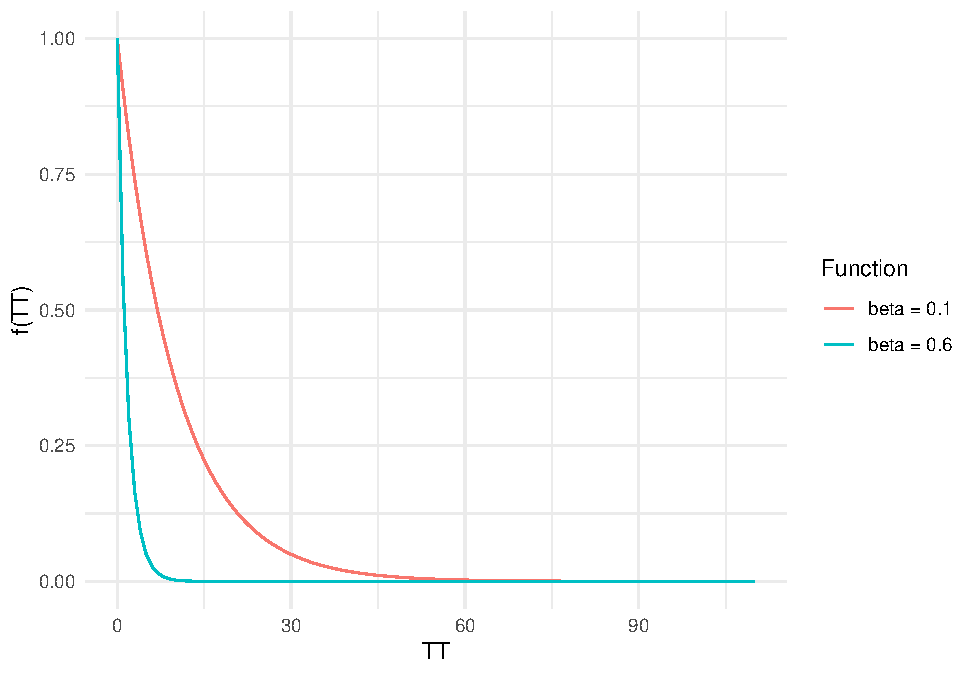
\includegraphics[width=1\linewidth]{Spatial-Availability-Refreshed_files/figure-latex/comparison-impedance-functions-synthetic-example-1} \caption{\label{fig:impedance-functions-comparison}Comparison of two impedance functions in the example.}\label{fig:comparison-impedance-functions-synthetic-example}
\end{figure}

 
  \providecommand{\huxb}[2]{\arrayrulecolor[RGB]{#1}\global\arrayrulewidth=#2pt}
  \providecommand{\huxvb}[2]{\color[RGB]{#1}\vrule width #2pt}
  \providecommand{\huxtpad}[1]{\rule{0pt}{#1}}
  \providecommand{\huxbpad}[1]{\rule[-#1]{0pt}{#1}}

\begin{table}[ht]
\begin{centerbox}
\begin{threeparttable}
\captionsetup{justification=centering,singlelinecheck=off}
\caption{Summary description of synthetic example: Hansen-type accessibility and Shen-type accessibility with competition with beta = 0.6}
 \label{tab:synthetic-example-2}
\setlength{\tabcolsep}{0pt}
\begin{tabularx}{1.3\textwidth}{p{0.13\textwidth} p{0.13\textwidth} p{0.13\textwidth} p{0.13\textwidth} p{0.13\textwidth} p{0.13\textwidth} p{0.13\textwidth} p{0.13\textwidth} p{0.13\textwidth} p{0.13\textwidth}}


\hhline{>{\huxb{190, 190, 190}{1}}|>{\huxb{190, 190, 190}{1}}|>{\huxb{190, 190, 190}{1}}|>{\huxb{190, 190, 190}{1}}|>{\huxb{190, 190, 190}{1}}|>{\huxb{190, 190, 190}{1}}|>{\huxb{190, 190, 190}{1}}|>{\huxb{190, 190, 190}{1}}|>{\huxb{190, 190, 190}{1}}|}
\arrayrulecolor{black}

\multicolumn{1}{!{\huxvb{0, 0, 0}{0}}p{0.13\textwidth}!{\huxvb{190, 190, 190}{1}}}{\hspace{6pt}\parbox[b]{0.13\textwidth-6pt-6pt}{\huxtpad{6pt + 1em}\raggedright \textbf{{\fontsize{7pt}{8.4pt}\selectfont Origin}}\huxbpad{6pt}}} &
\multicolumn{1}{p{0.13\textwidth}!{\huxvb{190, 190, 190}{1}}}{\hspace{6pt}\parbox[b]{0.13\textwidth-6pt-6pt}{\huxtpad{6pt + 1em}\centering \textbf{{\fontsize{7pt}{8.4pt}\selectfont Pop.}}\huxbpad{6pt}}} &
\multicolumn{1}{p{0.13\textwidth}!{\huxvb{190, 190, 190}{1}}}{\hspace{6pt}\parbox[b]{0.13\textwidth-6pt-6pt}{\huxtpad{6pt + 1em}\raggedright \textbf{{\fontsize{7pt}{8.4pt}\selectfont Dest.}}\huxbpad{6pt}}} &
\multicolumn{1}{p{0.13\textwidth}!{\huxvb{190, 190, 190}{1}}}{\hspace{6pt}\parbox[b]{0.13\textwidth-6pt-6pt}{\huxtpad{6pt + 1em}\centering \textbf{{\fontsize{7pt}{8.4pt}\selectfont Jobs}}\huxbpad{6pt}}} &
\multicolumn{1}{p{0.13\textwidth}!{\huxvb{190, 190, 190}{1}}}{\hspace{6pt}\parbox[b]{0.13\textwidth-6pt-6pt}{\huxtpad{6pt + 1em}\centering \textbf{{\fontsize{7pt}{8.4pt}\selectfont TT}}\huxbpad{6pt}}} &
\multicolumn{1}{p{0.13\textwidth}!{\huxvb{190, 190, 190}{1}}}{\hspace{6pt}\parbox[b]{0.13\textwidth-6pt-6pt}{\huxtpad{6pt + 1em}\centering \textbf{{\fontsize{7pt}{8.4pt}\selectfont f(TT)}}\huxbpad{6pt}}} &
\multicolumn{1}{p{0.13\textwidth}!{\huxvb{190, 190, 190}{1}}}{\hspace{6pt}\parbox[b]{0.13\textwidth-6pt-6pt}{\huxtpad{6pt + 1em}\centering \textbf{{\fontsize{7pt}{8.4pt}\selectfont Pop * f(TT)}}\huxbpad{6pt}}} &
\multicolumn{1}{p{0.13\textwidth}!{\huxvb{190, 190, 190}{1}}}{\hspace{6pt}\parbox[b]{0.13\textwidth-6pt-6pt}{\huxtpad{6pt + 1em}\centering \textbf{{\fontsize{7pt}{8.4pt}\selectfont Jobs * f(TT)}}\huxbpad{6pt}}} &
\multicolumn{1}{p{0.13\textwidth}!{\huxvb{190, 190, 190}{1}}}{\hspace{6pt}\parbox[b]{0.13\textwidth-6pt-6pt}{\huxtpad{6pt + 1em}\centering \textbf{{\fontsize{7pt}{8.4pt}\selectfont S\_i}}\huxbpad{6pt}}} &
\multicolumn{1}{p{0.13\textwidth}!{\huxvb{0, 0, 0}{0}}}{\hspace{6pt}\parbox[b]{0.13\textwidth-6pt-6pt}{\huxtpad{6pt + 1em}\centering \textbf{{\fontsize{7pt}{8.4pt}\selectfont a\_i}}\huxbpad{6pt}}} \tabularnewline[-0.5pt]


\hhline{>{\huxb{0, 0, 0}{0.4}}->{\huxb{0, 0, 0}{0.4}}->{\huxb{0, 0, 0}{0.4}}->{\huxb{0, 0, 0}{0.4}}->{\huxb{0, 0, 0}{0.4}}->{\huxb{0, 0, 0}{0.4}}->{\huxb{0, 0, 0}{0.4}}->{\huxb{0, 0, 0}{0.4}}->{\huxb{0, 0, 0}{0.4}}->{\huxb{0, 0, 0}{0.4}}-}
\arrayrulecolor{black}

\multicolumn{1}{!{\huxvb{0, 0, 0}{0}}p{0.13\textwidth}!{\huxvb{190, 190, 190}{1}}}{} &
\multicolumn{1}{p{0.13\textwidth}!{\huxvb{190, 190, 190}{1}}}{} &
\multicolumn{1}{p{0.13\textwidth}!{\huxvb{190, 190, 190}{1}}}{\hspace{6pt}\parbox[b]{0.13\textwidth-6pt-6pt}{\huxtpad{6pt + 1em}\raggedright {\fontsize{7pt}{8.4pt}\selectfont 1}\huxbpad{6pt}}} &
\multicolumn{1}{p{0.13\textwidth}!{\huxvb{190, 190, 190}{1}}}{\hspace{6pt}\parbox[b]{0.13\textwidth-6pt-6pt}{\huxtpad{6pt + 1em}\centering {\fontsize{7pt}{8.4pt}\selectfont 100,000}\huxbpad{6pt}}} &
\multicolumn{1}{p{0.13\textwidth}!{\huxvb{190, 190, 190}{1}}}{\hspace{6pt}\parbox[b]{0.13\textwidth-6pt-6pt}{\huxtpad{6pt + 1em}\centering {\fontsize{7pt}{8.4pt}\selectfont 15}\huxbpad{6pt}}} &
\multicolumn{1}{p{0.13\textwidth}!{\huxvb{190, 190, 190}{1}}}{\hspace{6pt}\parbox[b]{0.13\textwidth-6pt-6pt}{\huxtpad{6pt + 1em}\centering {\fontsize{7pt}{8.4pt}\selectfont $<$ 0.001}\huxbpad{6pt}}} &
\multicolumn{1}{p{0.13\textwidth}!{\huxvb{190, 190, 190}{1}}}{\hspace{6pt}\parbox[b]{0.13\textwidth-6pt-6pt}{\huxtpad{6pt + 1em}\centering {\fontsize{7pt}{8.4pt}\selectfont 6.17}\huxbpad{6pt}}} &
\multicolumn{1}{p{0.13\textwidth}!{\huxvb{190, 190, 190}{1}}}{\hspace{6pt}\parbox[b]{0.13\textwidth-6pt-6pt}{\huxtpad{6pt + 1em}\centering {\fontsize{7pt}{8.4pt}\selectfont 12.341}\huxbpad{6pt}}} &
\multicolumn{1}{p{0.13\textwidth}!{\huxvb{190, 190, 190}{1}}}{} &
\multicolumn{1}{p{0.13\textwidth}!{\huxvb{0, 0, 0}{0}}}{} \tabularnewline[-0.5pt]


\hhline{>{\huxb{190, 190, 190}{1}}|>{\huxb{190, 190, 190}{1}}|>{\huxb{190, 190, 190}{1}}|>{\huxb{190, 190, 190}{1}}|>{\huxb{190, 190, 190}{1}}|>{\huxb{190, 190, 190}{1}}|>{\huxb{190, 190, 190}{1}}|>{\huxb{190, 190, 190}{1}}|>{\huxb{190, 190, 190}{1}}|}
\arrayrulecolor{black}

\multicolumn{1}{!{\huxvb{0, 0, 0}{0}}p{0.13\textwidth}!{\huxvb{190, 190, 190}{1}}}{} &
\multicolumn{1}{p{0.13\textwidth}!{\huxvb{190, 190, 190}{1}}}{} &
\multicolumn{1}{p{0.13\textwidth}!{\huxvb{190, 190, 190}{1}}}{\hspace{6pt}\parbox[b]{0.13\textwidth-6pt-6pt}{\huxtpad{6pt + 1em}\raggedright {\fontsize{7pt}{8.4pt}\selectfont 2}\huxbpad{6pt}}} &
\multicolumn{1}{p{0.13\textwidth}!{\huxvb{190, 190, 190}{1}}}{\hspace{6pt}\parbox[b]{0.13\textwidth-6pt-6pt}{\huxtpad{6pt + 1em}\centering {\fontsize{7pt}{8.4pt}\selectfont 100,000}\huxbpad{6pt}}} &
\multicolumn{1}{p{0.13\textwidth}!{\huxvb{190, 190, 190}{1}}}{\hspace{6pt}\parbox[b]{0.13\textwidth-6pt-6pt}{\huxtpad{6pt + 1em}\centering {\fontsize{7pt}{8.4pt}\selectfont 30}\huxbpad{6pt}}} &
\multicolumn{1}{p{0.13\textwidth}!{\huxvb{190, 190, 190}{1}}}{\hspace{6pt}\parbox[b]{0.13\textwidth-6pt-6pt}{\huxtpad{6pt + 1em}\centering {\fontsize{7pt}{8.4pt}\selectfont $<$ 0.001}\huxbpad{6pt}}} &
\multicolumn{1}{p{0.13\textwidth}!{\huxvb{190, 190, 190}{1}}}{\hspace{6pt}\parbox[b]{0.13\textwidth-6pt-6pt}{\huxtpad{6pt + 1em}\centering {\fontsize{7pt}{8.4pt}\selectfont $<$ 0.001}\huxbpad{6pt}}} &
\multicolumn{1}{p{0.13\textwidth}!{\huxvb{190, 190, 190}{1}}}{\hspace{6pt}\parbox[b]{0.13\textwidth-6pt-6pt}{\huxtpad{6pt + 1em}\centering {\fontsize{7pt}{8.4pt}\selectfont 0.002}\huxbpad{6pt}}} &
\multicolumn{1}{p{0.13\textwidth}!{\huxvb{190, 190, 190}{1}}}{} &
\multicolumn{1}{p{0.13\textwidth}!{\huxvb{0, 0, 0}{0}}}{} \tabularnewline[-0.5pt]


\hhline{>{\huxb{190, 190, 190}{1}}|>{\huxb{190, 190, 190}{1}}|>{\huxb{190, 190, 190}{1}}|>{\huxb{190, 190, 190}{1}}|>{\huxb{190, 190, 190}{1}}|>{\huxb{190, 190, 190}{1}}|>{\huxb{190, 190, 190}{1}}|>{\huxb{190, 190, 190}{1}}|>{\huxb{190, 190, 190}{1}}|}
\arrayrulecolor{black}

\multicolumn{1}{!{\huxvb{0, 0, 0}{0}}p{0.13\textwidth}!{\huxvb{190, 190, 190}{1}}}{\multirow[t]{-3}{*}[0ex]{\hspace{6pt}\parbox[b]{0.13\textwidth-6pt-6pt}{\huxtpad{6pt + 1em}\raggedright {\fontsize{7pt}{8.4pt}\selectfont A}\huxbpad{6pt}}}} &
\multicolumn{1}{p{0.13\textwidth}!{\huxvb{190, 190, 190}{1}}}{\multirow[t]{-3}{*}[0ex]{\hspace{6pt}\parbox[b]{0.13\textwidth-6pt-6pt}{\huxtpad{6pt + 1em}\centering {\fontsize{7pt}{8.4pt}\selectfont 50,000}\huxbpad{6pt}}}} &
\multicolumn{1}{p{0.13\textwidth}!{\huxvb{190, 190, 190}{1}}}{\hspace{6pt}\parbox[b]{0.13\textwidth-6pt-6pt}{\huxtpad{6pt + 1em}\raggedright {\fontsize{7pt}{8.4pt}\selectfont 3}\huxbpad{6pt}}} &
\multicolumn{1}{p{0.13\textwidth}!{\huxvb{190, 190, 190}{1}}}{\hspace{6pt}\parbox[b]{0.13\textwidth-6pt-6pt}{\huxtpad{6pt + 1em}\centering {\fontsize{7pt}{8.4pt}\selectfont 10,000}\huxbpad{6pt}}} &
\multicolumn{1}{p{0.13\textwidth}!{\huxvb{190, 190, 190}{1}}}{\hspace{6pt}\parbox[b]{0.13\textwidth-6pt-6pt}{\huxtpad{6pt + 1em}\centering {\fontsize{7pt}{8.4pt}\selectfont 100}\huxbpad{6pt}}} &
\multicolumn{1}{p{0.13\textwidth}!{\huxvb{190, 190, 190}{1}}}{\hspace{6pt}\parbox[b]{0.13\textwidth-6pt-6pt}{\huxtpad{6pt + 1em}\centering {\fontsize{7pt}{8.4pt}\selectfont $<$ 0.001}\huxbpad{6pt}}} &
\multicolumn{1}{p{0.13\textwidth}!{\huxvb{190, 190, 190}{1}}}{\hspace{6pt}\parbox[b]{0.13\textwidth-6pt-6pt}{\huxtpad{6pt + 1em}\centering {\fontsize{7pt}{8.4pt}\selectfont $<$ 0.001}\huxbpad{6pt}}} &
\multicolumn{1}{p{0.13\textwidth}!{\huxvb{190, 190, 190}{1}}}{\hspace{6pt}\parbox[b]{0.13\textwidth-6pt-6pt}{\huxtpad{6pt + 1em}\centering {\fontsize{7pt}{8.4pt}\selectfont $<$ 0.001}\huxbpad{6pt}}} &
\multicolumn{1}{p{0.13\textwidth}!{\huxvb{190, 190, 190}{1}}}{\multirow[t]{-3}{*}[0ex]{\hspace{6pt}\parbox[b]{0.13\textwidth-6pt-6pt}{\huxtpad{6pt + 1em}\centering {\fontsize{7pt}{8.4pt}\selectfont 12.34}\huxbpad{6pt}}}} &
\multicolumn{1}{p{0.13\textwidth}!{\huxvb{0, 0, 0}{0}}}{\multirow[t]{-3}{*}[0ex]{\hspace{6pt}\parbox[b]{0.13\textwidth-6pt-6pt}{\huxtpad{6pt + 1em}\centering {\fontsize{7pt}{8.4pt}\selectfont 1.999}\huxbpad{6pt}}}} \tabularnewline[-0.5pt]


\hhline{>{\huxb{0, 0, 0}{0.4}}->{\huxb{0, 0, 0}{0.4}}->{\huxb{0, 0, 0}{0.4}}->{\huxb{0, 0, 0}{0.4}}->{\huxb{0, 0, 0}{0.4}}->{\huxb{0, 0, 0}{0.4}}->{\huxb{0, 0, 0}{0.4}}->{\huxb{0, 0, 0}{0.4}}->{\huxb{0, 0, 0}{0.4}}->{\huxb{0, 0, 0}{0.4}}-}
\arrayrulecolor{black}

\multicolumn{1}{!{\huxvb{0, 0, 0}{0}}p{0.13\textwidth}!{\huxvb{190, 190, 190}{1}}}{} &
\multicolumn{1}{p{0.13\textwidth}!{\huxvb{190, 190, 190}{1}}}{} &
\multicolumn{1}{p{0.13\textwidth}!{\huxvb{190, 190, 190}{1}}}{\hspace{6pt}\parbox[b]{0.13\textwidth-6pt-6pt}{\huxtpad{6pt + 1em}\raggedright {\fontsize{7pt}{8.4pt}\selectfont 1}\huxbpad{6pt}}} &
\multicolumn{1}{p{0.13\textwidth}!{\huxvb{190, 190, 190}{1}}}{\hspace{6pt}\parbox[b]{0.13\textwidth-6pt-6pt}{\huxtpad{6pt + 1em}\centering {\fontsize{7pt}{8.4pt}\selectfont 100,000}\huxbpad{6pt}}} &
\multicolumn{1}{p{0.13\textwidth}!{\huxvb{190, 190, 190}{1}}}{\hspace{6pt}\parbox[b]{0.13\textwidth-6pt-6pt}{\huxtpad{6pt + 1em}\centering {\fontsize{7pt}{8.4pt}\selectfont 30}\huxbpad{6pt}}} &
\multicolumn{1}{p{0.13\textwidth}!{\huxvb{190, 190, 190}{1}}}{\hspace{6pt}\parbox[b]{0.13\textwidth-6pt-6pt}{\huxtpad{6pt + 1em}\centering {\fontsize{7pt}{8.4pt}\selectfont $<$ 0.001}\huxbpad{6pt}}} &
\multicolumn{1}{p{0.13\textwidth}!{\huxvb{190, 190, 190}{1}}}{\hspace{6pt}\parbox[b]{0.13\textwidth-6pt-6pt}{\huxtpad{6pt + 1em}\centering {\fontsize{7pt}{8.4pt}\selectfont 0.002}\huxbpad{6pt}}} &
\multicolumn{1}{p{0.13\textwidth}!{\huxvb{190, 190, 190}{1}}}{\hspace{6pt}\parbox[b]{0.13\textwidth-6pt-6pt}{\huxtpad{6pt + 1em}\centering {\fontsize{7pt}{8.4pt}\selectfont 0.002}\huxbpad{6pt}}} &
\multicolumn{1}{p{0.13\textwidth}!{\huxvb{190, 190, 190}{1}}}{} &
\multicolumn{1}{p{0.13\textwidth}!{\huxvb{0, 0, 0}{0}}}{} \tabularnewline[-0.5pt]


\hhline{>{\huxb{190, 190, 190}{1}}|>{\huxb{190, 190, 190}{1}}|>{\huxb{190, 190, 190}{1}}|>{\huxb{190, 190, 190}{1}}|>{\huxb{190, 190, 190}{1}}|>{\huxb{190, 190, 190}{1}}|>{\huxb{190, 190, 190}{1}}|>{\huxb{190, 190, 190}{1}}|>{\huxb{190, 190, 190}{1}}|}
\arrayrulecolor{black}

\multicolumn{1}{!{\huxvb{0, 0, 0}{0}}p{0.13\textwidth}!{\huxvb{190, 190, 190}{1}}}{} &
\multicolumn{1}{p{0.13\textwidth}!{\huxvb{190, 190, 190}{1}}}{} &
\multicolumn{1}{p{0.13\textwidth}!{\huxvb{190, 190, 190}{1}}}{\hspace{6pt}\parbox[b]{0.13\textwidth-6pt-6pt}{\huxtpad{6pt + 1em}\raggedright {\fontsize{7pt}{8.4pt}\selectfont 2}\huxbpad{6pt}}} &
\multicolumn{1}{p{0.13\textwidth}!{\huxvb{190, 190, 190}{1}}}{\hspace{6pt}\parbox[b]{0.13\textwidth-6pt-6pt}{\huxtpad{6pt + 1em}\centering {\fontsize{7pt}{8.4pt}\selectfont 100,000}\huxbpad{6pt}}} &
\multicolumn{1}{p{0.13\textwidth}!{\huxvb{190, 190, 190}{1}}}{\hspace{6pt}\parbox[b]{0.13\textwidth-6pt-6pt}{\huxtpad{6pt + 1em}\centering {\fontsize{7pt}{8.4pt}\selectfont 15}\huxbpad{6pt}}} &
\multicolumn{1}{p{0.13\textwidth}!{\huxvb{190, 190, 190}{1}}}{\hspace{6pt}\parbox[b]{0.13\textwidth-6pt-6pt}{\huxtpad{6pt + 1em}\centering {\fontsize{7pt}{8.4pt}\selectfont $<$ 0.001}\huxbpad{6pt}}} &
\multicolumn{1}{p{0.13\textwidth}!{\huxvb{190, 190, 190}{1}}}{\hspace{6pt}\parbox[b]{0.13\textwidth-6pt-6pt}{\huxtpad{6pt + 1em}\centering {\fontsize{7pt}{8.4pt}\selectfont 18.511}\huxbpad{6pt}}} &
\multicolumn{1}{p{0.13\textwidth}!{\huxvb{190, 190, 190}{1}}}{\hspace{6pt}\parbox[b]{0.13\textwidth-6pt-6pt}{\huxtpad{6pt + 1em}\centering {\fontsize{7pt}{8.4pt}\selectfont 12.341}\huxbpad{6pt}}} &
\multicolumn{1}{p{0.13\textwidth}!{\huxvb{190, 190, 190}{1}}}{} &
\multicolumn{1}{p{0.13\textwidth}!{\huxvb{0, 0, 0}{0}}}{} \tabularnewline[-0.5pt]


\hhline{>{\huxb{190, 190, 190}{1}}|>{\huxb{190, 190, 190}{1}}|>{\huxb{190, 190, 190}{1}}|>{\huxb{190, 190, 190}{1}}|>{\huxb{190, 190, 190}{1}}|>{\huxb{190, 190, 190}{1}}|>{\huxb{190, 190, 190}{1}}|>{\huxb{190, 190, 190}{1}}|>{\huxb{190, 190, 190}{1}}|}
\arrayrulecolor{black}

\multicolumn{1}{!{\huxvb{0, 0, 0}{0}}p{0.13\textwidth}!{\huxvb{190, 190, 190}{1}}}{\multirow[t]{-3}{*}[0ex]{\hspace{6pt}\parbox[b]{0.13\textwidth-6pt-6pt}{\huxtpad{6pt + 1em}\raggedright {\fontsize{7pt}{8.4pt}\selectfont B}\huxbpad{6pt}}}} &
\multicolumn{1}{p{0.13\textwidth}!{\huxvb{190, 190, 190}{1}}}{\multirow[t]{-3}{*}[0ex]{\hspace{6pt}\parbox[b]{0.13\textwidth-6pt-6pt}{\huxtpad{6pt + 1em}\centering {\fontsize{7pt}{8.4pt}\selectfont 150,000}\huxbpad{6pt}}}} &
\multicolumn{1}{p{0.13\textwidth}!{\huxvb{190, 190, 190}{1}}}{\hspace{6pt}\parbox[b]{0.13\textwidth-6pt-6pt}{\huxtpad{6pt + 1em}\raggedright {\fontsize{7pt}{8.4pt}\selectfont 3}\huxbpad{6pt}}} &
\multicolumn{1}{p{0.13\textwidth}!{\huxvb{190, 190, 190}{1}}}{\hspace{6pt}\parbox[b]{0.13\textwidth-6pt-6pt}{\huxtpad{6pt + 1em}\centering {\fontsize{7pt}{8.4pt}\selectfont 10,000}\huxbpad{6pt}}} &
\multicolumn{1}{p{0.13\textwidth}!{\huxvb{190, 190, 190}{1}}}{\hspace{6pt}\parbox[b]{0.13\textwidth-6pt-6pt}{\huxtpad{6pt + 1em}\centering {\fontsize{7pt}{8.4pt}\selectfont 100}\huxbpad{6pt}}} &
\multicolumn{1}{p{0.13\textwidth}!{\huxvb{190, 190, 190}{1}}}{\hspace{6pt}\parbox[b]{0.13\textwidth-6pt-6pt}{\huxtpad{6pt + 1em}\centering {\fontsize{7pt}{8.4pt}\selectfont $<$ 0.001}\huxbpad{6pt}}} &
\multicolumn{1}{p{0.13\textwidth}!{\huxvb{190, 190, 190}{1}}}{\hspace{6pt}\parbox[b]{0.13\textwidth-6pt-6pt}{\huxtpad{6pt + 1em}\centering {\fontsize{7pt}{8.4pt}\selectfont $<$ 0.001}\huxbpad{6pt}}} &
\multicolumn{1}{p{0.13\textwidth}!{\huxvb{190, 190, 190}{1}}}{\hspace{6pt}\parbox[b]{0.13\textwidth-6pt-6pt}{\huxtpad{6pt + 1em}\centering {\fontsize{7pt}{8.4pt}\selectfont $<$ 0.001}\huxbpad{6pt}}} &
\multicolumn{1}{p{0.13\textwidth}!{\huxvb{190, 190, 190}{1}}}{\multirow[t]{-3}{*}[0ex]{\hspace{6pt}\parbox[b]{0.13\textwidth-6pt-6pt}{\huxtpad{6pt + 1em}\centering {\fontsize{7pt}{8.4pt}\selectfont 12.34}\huxbpad{6pt}}}} &
\multicolumn{1}{p{0.13\textwidth}!{\huxvb{0, 0, 0}{0}}}{\multirow[t]{-3}{*}[0ex]{\hspace{6pt}\parbox[b]{0.13\textwidth-6pt-6pt}{\huxtpad{6pt + 1em}\centering {\fontsize{7pt}{8.4pt}\selectfont 0.6669}\huxbpad{6pt}}}} \tabularnewline[-0.5pt]


\hhline{>{\huxb{0, 0, 0}{0.4}}->{\huxb{0, 0, 0}{0.4}}->{\huxb{0, 0, 0}{0.4}}->{\huxb{0, 0, 0}{0.4}}->{\huxb{0, 0, 0}{0.4}}->{\huxb{0, 0, 0}{0.4}}->{\huxb{0, 0, 0}{0.4}}->{\huxb{0, 0, 0}{0.4}}->{\huxb{0, 0, 0}{0.4}}->{\huxb{0, 0, 0}{0.4}}-}
\arrayrulecolor{black}

\multicolumn{1}{!{\huxvb{0, 0, 0}{0}}p{0.13\textwidth}!{\huxvb{190, 190, 190}{1}}}{} &
\multicolumn{1}{p{0.13\textwidth}!{\huxvb{190, 190, 190}{1}}}{} &
\multicolumn{1}{p{0.13\textwidth}!{\huxvb{190, 190, 190}{1}}}{\hspace{6pt}\parbox[b]{0.13\textwidth-6pt-6pt}{\huxtpad{6pt + 1em}\raggedright {\fontsize{7pt}{8.4pt}\selectfont 1}\huxbpad{6pt}}} &
\multicolumn{1}{p{0.13\textwidth}!{\huxvb{190, 190, 190}{1}}}{\hspace{6pt}\parbox[b]{0.13\textwidth-6pt-6pt}{\huxtpad{6pt + 1em}\centering {\fontsize{7pt}{8.4pt}\selectfont 100,000}\huxbpad{6pt}}} &
\multicolumn{1}{p{0.13\textwidth}!{\huxvb{190, 190, 190}{1}}}{\hspace{6pt}\parbox[b]{0.13\textwidth-6pt-6pt}{\huxtpad{6pt + 1em}\centering {\fontsize{7pt}{8.4pt}\selectfont 100}\huxbpad{6pt}}} &
\multicolumn{1}{p{0.13\textwidth}!{\huxvb{190, 190, 190}{1}}}{\hspace{6pt}\parbox[b]{0.13\textwidth-6pt-6pt}{\huxtpad{6pt + 1em}\centering {\fontsize{7pt}{8.4pt}\selectfont $<$ 0.001}\huxbpad{6pt}}} &
\multicolumn{1}{p{0.13\textwidth}!{\huxvb{190, 190, 190}{1}}}{\hspace{6pt}\parbox[b]{0.13\textwidth-6pt-6pt}{\huxtpad{6pt + 1em}\centering {\fontsize{7pt}{8.4pt}\selectfont $<$ 0.001}\huxbpad{6pt}}} &
\multicolumn{1}{p{0.13\textwidth}!{\huxvb{190, 190, 190}{1}}}{\hspace{6pt}\parbox[b]{0.13\textwidth-6pt-6pt}{\huxtpad{6pt + 1em}\centering {\fontsize{7pt}{8.4pt}\selectfont $<$ 0.001}\huxbpad{6pt}}} &
\multicolumn{1}{p{0.13\textwidth}!{\huxvb{190, 190, 190}{1}}}{} &
\multicolumn{1}{p{0.13\textwidth}!{\huxvb{0, 0, 0}{0}}}{} \tabularnewline[-0.5pt]


\hhline{>{\huxb{190, 190, 190}{1}}|>{\huxb{190, 190, 190}{1}}|>{\huxb{190, 190, 190}{1}}|>{\huxb{190, 190, 190}{1}}|>{\huxb{190, 190, 190}{1}}|>{\huxb{190, 190, 190}{1}}|>{\huxb{190, 190, 190}{1}}|>{\huxb{190, 190, 190}{1}}|>{\huxb{190, 190, 190}{1}}|}
\arrayrulecolor{black}

\multicolumn{1}{!{\huxvb{0, 0, 0}{0}}p{0.13\textwidth}!{\huxvb{190, 190, 190}{1}}}{} &
\multicolumn{1}{p{0.13\textwidth}!{\huxvb{190, 190, 190}{1}}}{} &
\multicolumn{1}{p{0.13\textwidth}!{\huxvb{190, 190, 190}{1}}}{\hspace{6pt}\parbox[b]{0.13\textwidth-6pt-6pt}{\huxtpad{6pt + 1em}\raggedright {\fontsize{7pt}{8.4pt}\selectfont 2}\huxbpad{6pt}}} &
\multicolumn{1}{p{0.13\textwidth}!{\huxvb{190, 190, 190}{1}}}{\hspace{6pt}\parbox[b]{0.13\textwidth-6pt-6pt}{\huxtpad{6pt + 1em}\centering {\fontsize{7pt}{8.4pt}\selectfont 100,000}\huxbpad{6pt}}} &
\multicolumn{1}{p{0.13\textwidth}!{\huxvb{190, 190, 190}{1}}}{\hspace{6pt}\parbox[b]{0.13\textwidth-6pt-6pt}{\huxtpad{6pt + 1em}\centering {\fontsize{7pt}{8.4pt}\selectfont 100}\huxbpad{6pt}}} &
\multicolumn{1}{p{0.13\textwidth}!{\huxvb{190, 190, 190}{1}}}{\hspace{6pt}\parbox[b]{0.13\textwidth-6pt-6pt}{\huxtpad{6pt + 1em}\centering {\fontsize{7pt}{8.4pt}\selectfont $<$ 0.001}\huxbpad{6pt}}} &
\multicolumn{1}{p{0.13\textwidth}!{\huxvb{190, 190, 190}{1}}}{\hspace{6pt}\parbox[b]{0.13\textwidth-6pt-6pt}{\huxtpad{6pt + 1em}\centering {\fontsize{7pt}{8.4pt}\selectfont $<$ 0.001}\huxbpad{6pt}}} &
\multicolumn{1}{p{0.13\textwidth}!{\huxvb{190, 190, 190}{1}}}{\hspace{6pt}\parbox[b]{0.13\textwidth-6pt-6pt}{\huxtpad{6pt + 1em}\centering {\fontsize{7pt}{8.4pt}\selectfont $<$ 0.001}\huxbpad{6pt}}} &
\multicolumn{1}{p{0.13\textwidth}!{\huxvb{190, 190, 190}{1}}}{} &
\multicolumn{1}{p{0.13\textwidth}!{\huxvb{0, 0, 0}{0}}}{} \tabularnewline[-0.5pt]


\hhline{>{\huxb{190, 190, 190}{1}}|>{\huxb{190, 190, 190}{1}}|>{\huxb{190, 190, 190}{1}}|>{\huxb{190, 190, 190}{1}}|>{\huxb{190, 190, 190}{1}}|>{\huxb{190, 190, 190}{1}}|>{\huxb{190, 190, 190}{1}}|>{\huxb{190, 190, 190}{1}}|>{\huxb{190, 190, 190}{1}}|}
\arrayrulecolor{black}

\multicolumn{1}{!{\huxvb{0, 0, 0}{0}}p{0.13\textwidth}!{\huxvb{190, 190, 190}{1}}}{\multirow[t]{-3}{*}[0ex]{\hspace{6pt}\parbox[b]{0.13\textwidth-6pt-6pt}{\huxtpad{6pt + 1em}\raggedright {\fontsize{7pt}{8.4pt}\selectfont C}\huxbpad{6pt}}}} &
\multicolumn{1}{p{0.13\textwidth}!{\huxvb{190, 190, 190}{1}}}{\multirow[t]{-3}{*}[0ex]{\hspace{6pt}\parbox[b]{0.13\textwidth-6pt-6pt}{\huxtpad{6pt + 1em}\centering {\fontsize{7pt}{8.4pt}\selectfont 10,000}\huxbpad{6pt}}}} &
\multicolumn{1}{p{0.13\textwidth}!{\huxvb{190, 190, 190}{1}}}{\hspace{6pt}\parbox[b]{0.13\textwidth-6pt-6pt}{\huxtpad{6pt + 1em}\raggedright {\fontsize{7pt}{8.4pt}\selectfont 3}\huxbpad{6pt}}} &
\multicolumn{1}{p{0.13\textwidth}!{\huxvb{190, 190, 190}{1}}}{\hspace{6pt}\parbox[b]{0.13\textwidth-6pt-6pt}{\huxtpad{6pt + 1em}\centering {\fontsize{7pt}{8.4pt}\selectfont 10,000}\huxbpad{6pt}}} &
\multicolumn{1}{p{0.13\textwidth}!{\huxvb{190, 190, 190}{1}}}{\hspace{6pt}\parbox[b]{0.13\textwidth-6pt-6pt}{\huxtpad{6pt + 1em}\centering {\fontsize{7pt}{8.4pt}\selectfont 15}\huxbpad{6pt}}} &
\multicolumn{1}{p{0.13\textwidth}!{\huxvb{190, 190, 190}{1}}}{\hspace{6pt}\parbox[b]{0.13\textwidth-6pt-6pt}{\huxtpad{6pt + 1em}\centering {\fontsize{7pt}{8.4pt}\selectfont $<$ 0.001}\huxbpad{6pt}}} &
\multicolumn{1}{p{0.13\textwidth}!{\huxvb{190, 190, 190}{1}}}{\hspace{6pt}\parbox[b]{0.13\textwidth-6pt-6pt}{\huxtpad{6pt + 1em}\centering {\fontsize{7pt}{8.4pt}\selectfont 1.234}\huxbpad{6pt}}} &
\multicolumn{1}{p{0.13\textwidth}!{\huxvb{190, 190, 190}{1}}}{\hspace{6pt}\parbox[b]{0.13\textwidth-6pt-6pt}{\huxtpad{6pt + 1em}\centering {\fontsize{7pt}{8.4pt}\selectfont 1.234}\huxbpad{6pt}}} &
\multicolumn{1}{p{0.13\textwidth}!{\huxvb{190, 190, 190}{1}}}{\multirow[t]{-3}{*}[0ex]{\hspace{6pt}\parbox[b]{0.13\textwidth-6pt-6pt}{\huxtpad{6pt + 1em}\centering {\fontsize{7pt}{8.4pt}\selectfont 1.234}\huxbpad{6pt}}}} &
\multicolumn{1}{p{0.13\textwidth}!{\huxvb{0, 0, 0}{0}}}{\multirow[t]{-3}{*}[0ex]{\hspace{6pt}\parbox[b]{0.13\textwidth-6pt-6pt}{\huxtpad{6pt + 1em}\centering {\fontsize{7pt}{8.4pt}\selectfont 1}\huxbpad{6pt}}}} \tabularnewline[-0.5pt]


\hhline{>{\huxb{190, 190, 190}{1}}|>{\huxb{190, 190, 190}{1}}|>{\huxb{190, 190, 190}{1}}|>{\huxb{190, 190, 190}{1}}|>{\huxb{190, 190, 190}{1}}|>{\huxb{190, 190, 190}{1}}|>{\huxb{190, 190, 190}{1}}|>{\huxb{190, 190, 190}{1}}|>{\huxb{190, 190, 190}{1}}|}
\arrayrulecolor{black}
\end{tabularx}
\end{threeparttable}\par\end{centerbox}

\end{table}
 

As expected, Hansen-type accessibility drops quite dramatically after
this \(\beta\) modification: the friction of distance is so high that
few opportunities are within reach. In contrast, Shen-type accessibility
converges to the jobs:population ratio (i.e., origin \(A\) is
\(\frac{100,000}{50,000} = 2\)). This is explained by the way the
impedance function excludes the population in droves, thus reducing the
competition for jobs: as seen in Table \ref{tab:synthetic-example-2},
the effective opportunity-seeking population from \(A\) is only about
6.17; likewise, the number of jobs at 1 weighted by the impedance is
only 12.341. In other words, competition is low because jobs are
expensive to reach, but those willing to reach jobs enjoy relatively
high accessibility (in the limit, the jobs/population ratio). On the
other hand, the accessibility is effectively zero for those in the
population prevented by the impedance from reaching any jobs.

In what follows, we propose an alternative derivation of
\citet{shen1998} accessibility with competition that explicitly
clarifies the opportunities allocated to the \emph{effective
opportunity-seeking population} within its formulation. Hence, the
results are not only more interpretable, also extend the potential of
accessibility analysis.

\hypertarget{introducing-spatial-availability-a-singly-constrained-measure-of-accessibility}{%
\section{Introducing spatial availability: a singly-constrained measure
of
accessibility}\label{introducing-spatial-availability-a-singly-constrained-measure-of-accessibility}}

In brief, we define the \emph{spatial availability} at \(i\) (\(V_{i}\))
as the proportion of all opportunities \(O\) that are allocated to \(i\)
from all destinations \(j\): \[
V_i = \sum_{j=1}^KO_jF^t_{ij}
\]

\noindent where:

\begin{itemize}
\tightlist
\item
  \(F^t_{ij}\) is a balancing factor that depends on the population and
  cost of movement in the system.
\item
  \(O_j\) is the number of opportunities at \(j\).
\item
  \(V_i\) is the number of spatially available opportunities from the
  perspective of \(i\).
\end{itemize}

The general form of spatial availability is also as a sum, and the
fundamental difference with Hansen- and Shen-type accessibility is that
opportunities are allocated proportionally. Balancing factor
\(F^t_{ij}\) consists of two components: a population-based balancing
factor \(F^p_{i}\) and an impedance-based balancing factor \(F^c_{ij}\)
which, respectively, allocate opportunities to \(i\) in proportion to
the size of the population of the different competing centers (the mass
effect of the gravity model) and the cost of reaching opportunities (the
impedance effect). In the next two subsections, we explain the intuition
behind the method before defining it in full.

\hypertarget{proportional-allocation-by-population}{%
\subsection{Proportional allocation by
population}\label{proportional-allocation-by-population}}

According to the gravity modelling framework, the potential for
interaction depends on the mass (i.e., the population) and the friction
of distance (i.e., the impedance function). We begin by describing the
proposed proportional allocation mechanism based on demand by
population. Recall, the total population in the example is 210,000. The
proportion of the population by population center is as follows: \[
\begin{array}{l}
F^p_A = \frac{50,000}{210,000}\\
\\
F^p_B = \frac{150,000}{210,000}\\
\\
F^p_C = \frac{10,000}{210,000}\\
\end{array}
\]

Jobs are allocated proportionally from each employment center to each
population center depending on their population sizes as per the
balancing factors \(F^p_i\). In this way, employment center 1 allocates
\(100,000\cdot \frac{50,000}{210,000}= 23,809.52\) jobs to \(A\);
\(100,000\cdot \frac{150,000}{210,000}= 71,428.57\) jobs to \(B\); and
\(100,000\cdot \frac{10,000}{210,000}= 7,142.857\) jobs to \(C\). Notice
how this mechanism ensures that the total number of jobs at employment
center 1 is preserved at 100,000.

We can verify that the number of jobs allocated is consistent with the
total number of jobs in the system: \[
\begin{array}{l}
\text{Employment center 1 to population centers A, B, and C: }\\
100,000 \cdot \frac{50,000}{210,000} + 100,000 \cdot \frac{150,000}{210,000} + 100,000 \cdot \frac{10,000}{210,000} = 100,000\\
\\
\text{Employment center 2 to population centers A, B, and C: }\\
100,000 \cdot \frac{50,000}{210,000} + 100,000 \cdot \frac{150,000}{210,000} + 100,000 \cdot \frac{10,000}{210,000} = 100,000\\
\\
\text{Employment center 3 to population centers A, B, and C: }\\
10,000 \cdot \frac{50,000}{210,000} + 10,000 \cdot \frac{150,000}{210,000} + 10,000 \cdot \frac{10,000}{210,000} = 10,000\\
\end{array}
\]

In the general case where there are \(N\) population centers in the
region, we define the following population-based balancing factors:

\begin{equation}
\label{eq:population-balancing-factor}
F^p_{i} = \frac{P_{i}^\alpha}{\sum_{i=1}^N P_{i}^\alpha}
\end{equation}

Balancing factor \(F^p_{i}\) corresponds to the proportion of the
population in origin \(i\) relative to the population in the region. On
the right hand side of the equation, the numerator \(P_{i}^\alpha\) is
the population at origin \(i\). The summation in the denominator is over
\(i=1,\cdots,N\), and adds up to the total population of the region.
Notice that we incorporate an empirical parameter \(\alpha\). The role
of \(\alpha\) is to modulate the effect of demand by population. When
\(\alpha <1\), opportunities are allocated more rapidly to smaller
centers relative to larger ones; \(\alpha>1\) achieves the opposite
effect.

Balancing factor \(F^p_{i}\) can now be used to proportionally allocate
a share of available jobs at \(j\) to origin \(i\). The number of jobs
available to \(i\) from \(j\) balanced by population shares is defined
as follows: \[
V^p_{ij} = O_j\frac{F^p_{i}}{\sum_{i=1}^K F^p_{i}}
\]

In the general case where there are \(J\) employment centers, the total
number of jobs available from all destinations to \(i\) is simply the
sum of \(V^p_{ij}\) over \(j=1,\cdots, J\): \[
V^p_{i} = \sum_{j=1}^J O_j\frac{F^p_{i}}{\sum_{i=1}^K F^p_{i}}
\]

Since the factor \(F^p_{i}\), when summed over \(i=1,\cdots,N\) always
equals to 1 (i.e., \(\sum_{i=1}^{N} F^p_{i} = 1\)), the sum of all
spatially available jobs equals \(O\), the total number of opportunities
in the region: \[
\begin{array}{l}
\sum_{i=1}^N V^p_i =\sum_{i=1}^N\sum_{j=1}^JO_j\frac{F^p_{i}}{\sum_{i=1}^N F^p_{i}}\\
=\sum_{i=1}^N \frac{F^p_{i}}{\sum_{i=1}^N F^p_{i}}\cdot\sum_{j=1}^JO_j\\
=\sum_{j=1}^J O_j = O
\end{array}
\] The terms \(F^p_{i}\) act here as the balancing factors of the
gravity model when a single constraint is imposed \citep[i.e., to ensure
that the sums of columns are equal to the number of opportunities per
destination, see][pp.~179-180 and 183-184]{ortuzar_2011_modelling}. As a
result, the sum of spatial availability for all population centers
equals the total number of opportunities.

The discussion so far concerns only the mass effect (i.e., population
size) of the gravity model. In addition, the potential for interaction
is thought to decrease with increasing cost, so next we define similar
balancing factors but based on the impedance.

\hypertarget{proportional-allocation-by-cost}{%
\subsection{Proportional allocation by
cost}\label{proportional-allocation-by-cost}}

Clearly, using only balancing factors \(F^p_{i}\) to calculate spatial
availability \(V^p_i\) does not account for the cost of reaching
employment centers. Consider instead a set of balancing factors
\(F^c_{ij}\) that account for the friction of distance for our example.
Recall that the impedance function \(f(c_{ij})\) equals
\(\exp(-\beta\cdot c_{ij})\) where \(\beta = 0.1\) and travel time
\(c_{ij}\) is either 15, 30 or 60 minutes. For instance, the
impedance-based balancing factors \(F^c_{ij}\) would be the following
for employment center 1 (employment center 2 and 3 have their own
balancing factor values for each origin \(i\) as will be discussed
later): \[
\begin{array}{l}
F^c_{A1} = \frac{0.223130}{0.223130 + 0.049787 + 0.000045} = 0.8174398\\
F^c_{B1} = \frac{0.049787}{0.223130 + 0.049787 + 0.000045} = 0.1823954\\
F^c_{C1} = \frac{0.000045}{0.223130 + 0.049787 + 0.000045} = 0.0001648581\\
\end{array}
\]

Balancing factors \(F^c_{ij}\) use the impedance function to
proportionally allocate more jobs to closer population centers, that is,
to those with populations \emph{more willing to reach the jobs}. Indeed,
the factors \(F^c_{ij}\) can be thought of as the proportion of the
population at \(i\) willing to travel to destination \(j\), conditional
on the travel behavior as given by the impedance function. For instance,
\({81.74398}\%\) of jobs from employment center 1 are allocated to
population center \(A\) based on impedance.

So as follows from our example, of the 100,000 jobs at employment center
1 the number of jobs allocated to population center \(A\) is
\(100,000\times 0.8174398 = 81,743.98\) jobs; the number allocated to
population center \(B\) is \(100,000\times 0.1823954 = 18,239.54\) jobs;
and the number allocated to population center \(C\) is
\(100,000\times 0.0001648581 = 16.48581\) jobs. We see once more that
the total number of jobs at the employment center is preserved at
100,000. In this example, the proportional allocation mechanism assigns
the largest share of jobs to population center \(A\), which is the
closest to employment center 1, and the smallest to the more distant
population center \(C\).

In the general case where there are \(N\) population centers and \(J\)
employment centers in the region, we define the following
impedance-based balancing factors:

\begin{equation}
\label{eq:impedance-balancing-factor}
F^c_{ij} = \frac{f(c_{ij})}{\sum_{i=1}^N f(c_{ij})}\\
\end{equation}

The total number of jobs available to \(i\) from \(j\) according to
impedance is defined as follows: \[
V^c_{ij} = O_j\frac{F^c_{i}}{\sum_{i=1}^N F^c_{i}}
\]

The total number of jobs available to \(i\) from all destinations is: \[
V^c_{i} = \sum_{j=1}^J O_j\frac{F^c_{i}}{\sum_{i=1}^N F^c_{i}}
\]

Like the population-based allocation factors, \(F^c_{i}\) summed over
\(i=1,\cdots,N\) always equals to 1 (i.e.,
\(\sum_{i=1}^{N} F^c_{i} = 1\)). As before, the sum of all spatially
available jobs equals \(O\), the total number of opportunities in the
region: \[
\begin{array}{l}
\sum_{i=1}^N V^c_i =\sum_{i=1}^N\sum_{j=1}^JO_j\frac{F^c_{i}}{\sum_{i=1}^N F^c_{i}}\\
=\sum_{i=1}^N \frac{F^c_{i}}{\sum_{i=1}^N F^c_{i}}\cdot\sum_{j=1}^JO_j\\
=\sum_{j=1}^J O_j = O
\end{array}
\]

We are now ready to more formally define spatial availability with due
consideration to both population and travel cost effects.

\hypertarget{assembling-mass-and-impedance-effects}{%
\subsection{Assembling mass and impedance
effects}\label{assembling-mass-and-impedance-effects}}

Population and the cost of travel are both part of the gravity modelling
framework. Since the balancing factors defined in the preceding sections
are proportions (alternatively, can be understood as probabilities),
they can be combined multiplicatively to obtain their joint effect. This
multiplicative relationship can alternatively be understood as the joint
probability of allocating opportunities and is captured by Equation
(\ref{eq:balancing-factors}), where \(F^p_{i}\) is the population-based
balancing factor that grants a larger share of the existing
opportunities to larger centers and \(F^c_{ij}\) is the impedance-based
balancing factor that grants a larger share of the existing
opportunities to closer centers. This is in line with the tradition of
gravity modeling.

\begin{equation}
\label{eq:balancing-factors}
F^t_{ij} = \frac{F^p_{i} \cdot F^c_{ij}}{\sum_{i=1}^N F^p_{i} \cdot F^c_{ij}}
\end{equation}

\noindent with \(F^p_{i}\) and \(F^c_{ij}\) as defined in Equations
(\ref{eq:population-balancing-factor}) and
(\ref{eq:impedance-balancing-factor}) respectively. The combined
balancing factor \(F^t_{ij}\) is used to proportionally allocate jobs
from \(j\) to \(i\). Hence, spatial availability is given by Equation
(\ref{eq:spatial-availability}).

\begin{equation}
\label{eq:spatial-availability}
V_{i} = \sum_{j=1}^J O_j\ F^t_{ij}
\end{equation}

The terms in Equation \ref{eq:spatial-availability} are as follows:

\begin{itemize}
\tightlist
\item
  \(F^t_{ij}\) is a balancing factor as defined in Equation
  (\ref{eq:balancing-factors}).
\item
  \(i\) is a set of origin locations in the region \(i = 1,\cdots, N\).
\item
  \(j\) is a set of destination locations in the region
  \(j = 1,\cdots,J\).
\item
  \(O_j\) is the number of opportunities at location \(j\).
\item
  \(V_{i}\) is the spatial availability at \(i\).
\end{itemize}

Notice that, unlike \(S_i\) in Hansen-type accessibility (Equation
(\ref{eq:conventional-accessibility})), the population enters the
calculation of \(V_{i}\) through \(F^p_i\). Returning to Shen's example
in Figure \ref{fig:plot-toy-example}, Table
\ref{tab:synthetic-example-spatial-availability} contains the
information needed to calculate \(V_i\), with \(\beta\) set again to 0.1
as in Table \ref{tab:synthetic-example}.

 
  \providecommand{\huxb}[2]{\arrayrulecolor[RGB]{#1}\global\arrayrulewidth=#2pt}
  \providecommand{\huxvb}[2]{\color[RGB]{#1}\vrule width #2pt}
  \providecommand{\huxtpad}[1]{\rule{0pt}{#1}}
  \providecommand{\huxbpad}[1]{\rule[-#1]{0pt}{#1}}

\begin{table}[ht]
\begin{centerbox}
\begin{threeparttable}
\captionsetup{justification=centering,singlelinecheck=off}
\caption{Summary description of synthetic example: spatial availability}
 \label{tab:synthetic-example-spatial-availability}
\setlength{\tabcolsep}{0pt}
\begin{tabularx}{1.2\textwidth}{p{0.109090909090909\textwidth} p{0.109090909090909\textwidth} p{0.109090909090909\textwidth} p{0.109090909090909\textwidth} p{0.109090909090909\textwidth} p{0.109090909090909\textwidth} p{0.109090909090909\textwidth} p{0.109090909090909\textwidth} p{0.109090909090909\textwidth} p{0.109090909090909\textwidth} p{0.109090909090909\textwidth}}


\hhline{>{\huxb{190, 190, 190}{1}}|>{\huxb{190, 190, 190}{1}}|>{\huxb{190, 190, 190}{1}}|>{\huxb{190, 190, 190}{1}}|>{\huxb{190, 190, 190}{1}}|>{\huxb{190, 190, 190}{1}}|>{\huxb{190, 190, 190}{1}}|>{\huxb{190, 190, 190}{1}}|>{\huxb{190, 190, 190}{1}}|>{\huxb{190, 190, 190}{1}}|}
\arrayrulecolor{black}

\multicolumn{1}{!{\huxvb{0, 0, 0}{0}}p{0.109090909090909\textwidth}!{\huxvb{190, 190, 190}{1}}}{\hspace{6pt}\parbox[b]{0.109090909090909\textwidth-6pt-6pt}{\huxtpad{6pt + 1em}\raggedright \textbf{{\fontsize{7pt}{8.4pt}\selectfont Origin}}\huxbpad{6pt}}} &
\multicolumn{1}{p{0.109090909090909\textwidth}!{\huxvb{190, 190, 190}{1}}}{\hspace{6pt}\parbox[b]{0.109090909090909\textwidth-6pt-6pt}{\huxtpad{6pt + 1em}\centering \textbf{{\fontsize{7pt}{8.4pt}\selectfont Pop.}}\huxbpad{6pt}}} &
\multicolumn{1}{p{0.109090909090909\textwidth}!{\huxvb{190, 190, 190}{1}}}{\hspace{6pt}\parbox[b]{0.109090909090909\textwidth-6pt-6pt}{\huxtpad{6pt + 1em}\raggedright \textbf{{\fontsize{7pt}{8.4pt}\selectfont Dest.}}\huxbpad{6pt}}} &
\multicolumn{1}{p{0.109090909090909\textwidth}!{\huxvb{190, 190, 190}{1}}}{\hspace{6pt}\parbox[b]{0.109090909090909\textwidth-6pt-6pt}{\huxtpad{6pt + 1em}\centering \textbf{{\fontsize{7pt}{8.4pt}\selectfont Jobs}}\huxbpad{6pt}}} &
\multicolumn{1}{p{0.109090909090909\textwidth}!{\huxvb{190, 190, 190}{1}}}{\hspace{6pt}\parbox[b]{0.109090909090909\textwidth-6pt-6pt}{\huxtpad{6pt + 1em}\centering \textbf{{\fontsize{7pt}{8.4pt}\selectfont TT}}\huxbpad{6pt}}} &
\multicolumn{1}{p{0.109090909090909\textwidth}!{\huxvb{190, 190, 190}{1}}}{\hspace{6pt}\parbox[b]{0.109090909090909\textwidth-6pt-6pt}{\huxtpad{6pt + 1em}\centering \textbf{{\fontsize{7pt}{8.4pt}\selectfont f(TT)}}\huxbpad{6pt}}} &
\multicolumn{1}{p{0.109090909090909\textwidth}!{\huxvb{190, 190, 190}{1}}}{\hspace{6pt}\parbox[b]{0.109090909090909\textwidth-6pt-6pt}{\huxtpad{6pt + 1em}\centering \textbf{{\fontsize{7pt}{8.4pt}\selectfont F\textasciicircum p}}\huxbpad{6pt}}} &
\multicolumn{1}{p{0.109090909090909\textwidth}!{\huxvb{190, 190, 190}{1}}}{\hspace{6pt}\parbox[b]{0.109090909090909\textwidth-6pt-6pt}{\huxtpad{6pt + 1em}\centering \textbf{{\fontsize{7pt}{8.4pt}\selectfont F\textasciicircum c}}\huxbpad{6pt}}} &
\multicolumn{1}{p{0.109090909090909\textwidth}!{\huxvb{190, 190, 190}{1}}}{\hspace{6pt}\parbox[b]{0.109090909090909\textwidth-6pt-6pt}{\huxtpad{6pt + 1em}\centering \textbf{{\fontsize{7pt}{8.4pt}\selectfont F}}\huxbpad{6pt}}} &
\multicolumn{1}{p{0.109090909090909\textwidth}!{\huxvb{190, 190, 190}{1}}}{\hspace{6pt}\parbox[b]{0.109090909090909\textwidth-6pt-6pt}{\huxtpad{6pt + 1em}\centering \textbf{{\fontsize{7pt}{8.4pt}\selectfont V\_ij}}\huxbpad{6pt}}} &
\multicolumn{1}{p{0.109090909090909\textwidth}!{\huxvb{0, 0, 0}{0}}}{\hspace{6pt}\parbox[b]{0.109090909090909\textwidth-6pt-6pt}{\huxtpad{6pt + 1em}\raggedleft \textbf{{\fontsize{7pt}{8.4pt}\selectfont V\_i}}\huxbpad{6pt}}} \tabularnewline[-0.5pt]


\hhline{>{\huxb{0, 0, 0}{0.4}}->{\huxb{0, 0, 0}{0.4}}->{\huxb{0, 0, 0}{0.4}}->{\huxb{0, 0, 0}{0.4}}->{\huxb{0, 0, 0}{0.4}}->{\huxb{0, 0, 0}{0.4}}->{\huxb{0, 0, 0}{0.4}}->{\huxb{0, 0, 0}{0.4}}->{\huxb{0, 0, 0}{0.4}}->{\huxb{0, 0, 0}{0.4}}->{\huxb{0, 0, 0}{0.4}}-}
\arrayrulecolor{black}

\multicolumn{1}{!{\huxvb{0, 0, 0}{0}}p{0.109090909090909\textwidth}!{\huxvb{190, 190, 190}{1}}}{} &
\multicolumn{1}{p{0.109090909090909\textwidth}!{\huxvb{190, 190, 190}{1}}}{} &
\multicolumn{1}{p{0.109090909090909\textwidth}!{\huxvb{190, 190, 190}{1}}}{\hspace{6pt}\parbox[b]{0.109090909090909\textwidth-6pt-6pt}{\huxtpad{6pt + 1em}\raggedright {\fontsize{7pt}{8.4pt}\selectfont 1}\huxbpad{6pt}}} &
\multicolumn{1}{p{0.109090909090909\textwidth}!{\huxvb{190, 190, 190}{1}}}{\hspace{6pt}\parbox[b]{0.109090909090909\textwidth-6pt-6pt}{\huxtpad{6pt + 1em}\centering {\fontsize{7pt}{8.4pt}\selectfont 100,000}\huxbpad{6pt}}} &
\multicolumn{1}{p{0.109090909090909\textwidth}!{\huxvb{190, 190, 190}{1}}}{\hspace{6pt}\parbox[b]{0.109090909090909\textwidth-6pt-6pt}{\huxtpad{6pt + 1em}\centering {\fontsize{7pt}{8.4pt}\selectfont 15}\huxbpad{6pt}}} &
\multicolumn{1}{p{0.109090909090909\textwidth}!{\huxvb{190, 190, 190}{1}}}{\hspace{6pt}\parbox[b]{0.109090909090909\textwidth-6pt-6pt}{\huxtpad{6pt + 1em}\centering {\fontsize{7pt}{8.4pt}\selectfont 0.223130}\huxbpad{6pt}}} &
\multicolumn{1}{p{0.109090909090909\textwidth}!{\huxvb{190, 190, 190}{1}}}{\hspace{6pt}\parbox[b]{0.109090909090909\textwidth-6pt-6pt}{\huxtpad{6pt + 1em}\centering {\fontsize{7pt}{8.4pt}\selectfont 0.238095}\huxbpad{6pt}}} &
\multicolumn{1}{p{0.109090909090909\textwidth}!{\huxvb{190, 190, 190}{1}}}{\hspace{6pt}\parbox[b]{0.109090909090909\textwidth-6pt-6pt}{\huxtpad{6pt + 1em}\centering {\fontsize{7pt}{8.4pt}\selectfont 0.817438}\huxbpad{6pt}}} &
\multicolumn{1}{p{0.109090909090909\textwidth}!{\huxvb{190, 190, 190}{1}}}{\hspace{6pt}\parbox[b]{0.109090909090909\textwidth-6pt-6pt}{\huxtpad{6pt + 1em}\centering {\fontsize{7pt}{8.4pt}\selectfont 0.599006}\huxbpad{6pt}}} &
\multicolumn{1}{p{0.109090909090909\textwidth}!{\huxvb{190, 190, 190}{1}}}{\hspace{6pt}\parbox[b]{0.109090909090909\textwidth-6pt-6pt}{\huxtpad{6pt + 1em}\centering {\fontsize{7pt}{8.4pt}\selectfont 59,901}\huxbpad{6pt}}} &
\multicolumn{1}{p{0.109090909090909\textwidth}!{\huxvb{0, 0, 0}{0}}}{} \tabularnewline[-0.5pt]


\hhline{>{\huxb{190, 190, 190}{1}}|>{\huxb{190, 190, 190}{1}}|>{\huxb{190, 190, 190}{1}}|>{\huxb{190, 190, 190}{1}}|>{\huxb{190, 190, 190}{1}}|>{\huxb{190, 190, 190}{1}}|>{\huxb{190, 190, 190}{1}}|>{\huxb{190, 190, 190}{1}}|>{\huxb{190, 190, 190}{1}}|>{\huxb{190, 190, 190}{1}}|}
\arrayrulecolor{black}

\multicolumn{1}{!{\huxvb{0, 0, 0}{0}}p{0.109090909090909\textwidth}!{\huxvb{190, 190, 190}{1}}}{} &
\multicolumn{1}{p{0.109090909090909\textwidth}!{\huxvb{190, 190, 190}{1}}}{} &
\multicolumn{1}{p{0.109090909090909\textwidth}!{\huxvb{190, 190, 190}{1}}}{\hspace{6pt}\parbox[b]{0.109090909090909\textwidth-6pt-6pt}{\huxtpad{6pt + 1em}\raggedright {\fontsize{7pt}{8.4pt}\selectfont 2}\huxbpad{6pt}}} &
\multicolumn{1}{p{0.109090909090909\textwidth}!{\huxvb{190, 190, 190}{1}}}{\hspace{6pt}\parbox[b]{0.109090909090909\textwidth-6pt-6pt}{\huxtpad{6pt + 1em}\centering {\fontsize{7pt}{8.4pt}\selectfont 100,000}\huxbpad{6pt}}} &
\multicolumn{1}{p{0.109090909090909\textwidth}!{\huxvb{190, 190, 190}{1}}}{\hspace{6pt}\parbox[b]{0.109090909090909\textwidth-6pt-6pt}{\huxtpad{6pt + 1em}\centering {\fontsize{7pt}{8.4pt}\selectfont 30}\huxbpad{6pt}}} &
\multicolumn{1}{p{0.109090909090909\textwidth}!{\huxvb{190, 190, 190}{1}}}{\hspace{6pt}\parbox[b]{0.109090909090909\textwidth-6pt-6pt}{\huxtpad{6pt + 1em}\centering {\fontsize{7pt}{8.4pt}\selectfont 0.049787}\huxbpad{6pt}}} &
\multicolumn{1}{p{0.109090909090909\textwidth}!{\huxvb{190, 190, 190}{1}}}{\hspace{6pt}\parbox[b]{0.109090909090909\textwidth-6pt-6pt}{\huxtpad{6pt + 1em}\centering {\fontsize{7pt}{8.4pt}\selectfont 0.238095}\huxbpad{6pt}}} &
\multicolumn{1}{p{0.109090909090909\textwidth}!{\huxvb{190, 190, 190}{1}}}{\hspace{6pt}\parbox[b]{0.109090909090909\textwidth-6pt-6pt}{\huxtpad{6pt + 1em}\centering {\fontsize{7pt}{8.4pt}\selectfont 0.182395}\huxbpad{6pt}}} &
\multicolumn{1}{p{0.109090909090909\textwidth}!{\huxvb{190, 190, 190}{1}}}{\hspace{6pt}\parbox[b]{0.109090909090909\textwidth-6pt-6pt}{\huxtpad{6pt + 1em}\centering {\fontsize{7pt}{8.4pt}\selectfont 0.069227}\huxbpad{6pt}}} &
\multicolumn{1}{p{0.109090909090909\textwidth}!{\huxvb{190, 190, 190}{1}}}{\hspace{6pt}\parbox[b]{0.109090909090909\textwidth-6pt-6pt}{\huxtpad{6pt + 1em}\centering {\fontsize{7pt}{8.4pt}\selectfont 6,923}\huxbpad{6pt}}} &
\multicolumn{1}{p{0.109090909090909\textwidth}!{\huxvb{0, 0, 0}{0}}}{} \tabularnewline[-0.5pt]


\hhline{>{\huxb{190, 190, 190}{1}}|>{\huxb{190, 190, 190}{1}}|>{\huxb{190, 190, 190}{1}}|>{\huxb{190, 190, 190}{1}}|>{\huxb{190, 190, 190}{1}}|>{\huxb{190, 190, 190}{1}}|>{\huxb{190, 190, 190}{1}}|>{\huxb{190, 190, 190}{1}}|>{\huxb{190, 190, 190}{1}}|>{\huxb{190, 190, 190}{1}}|}
\arrayrulecolor{black}

\multicolumn{1}{!{\huxvb{0, 0, 0}{0}}p{0.109090909090909\textwidth}!{\huxvb{190, 190, 190}{1}}}{\multirow[t]{-3}{*}[0ex]{\hspace{6pt}\parbox[b]{0.109090909090909\textwidth-6pt-6pt}{\huxtpad{6pt + 1em}\raggedright {\fontsize{7pt}{8.4pt}\selectfont A}\huxbpad{6pt}}}} &
\multicolumn{1}{p{0.109090909090909\textwidth}!{\huxvb{190, 190, 190}{1}}}{\multirow[t]{-3}{*}[0ex]{\hspace{6pt}\parbox[b]{0.109090909090909\textwidth-6pt-6pt}{\huxtpad{6pt + 1em}\centering {\fontsize{7pt}{8.4pt}\selectfont 50,000}\huxbpad{6pt}}}} &
\multicolumn{1}{p{0.109090909090909\textwidth}!{\huxvb{190, 190, 190}{1}}}{\hspace{6pt}\parbox[b]{0.109090909090909\textwidth-6pt-6pt}{\huxtpad{6pt + 1em}\raggedright {\fontsize{7pt}{8.4pt}\selectfont 3}\huxbpad{6pt}}} &
\multicolumn{1}{p{0.109090909090909\textwidth}!{\huxvb{190, 190, 190}{1}}}{\hspace{6pt}\parbox[b]{0.109090909090909\textwidth-6pt-6pt}{\huxtpad{6pt + 1em}\centering {\fontsize{7pt}{8.4pt}\selectfont 10,000}\huxbpad{6pt}}} &
\multicolumn{1}{p{0.109090909090909\textwidth}!{\huxvb{190, 190, 190}{1}}}{\hspace{6pt}\parbox[b]{0.109090909090909\textwidth-6pt-6pt}{\huxtpad{6pt + 1em}\centering {\fontsize{7pt}{8.4pt}\selectfont 100}\huxbpad{6pt}}} &
\multicolumn{1}{p{0.109090909090909\textwidth}!{\huxvb{190, 190, 190}{1}}}{\hspace{6pt}\parbox[b]{0.109090909090909\textwidth-6pt-6pt}{\huxtpad{6pt + 1em}\centering {\fontsize{7pt}{8.4pt}\selectfont 0.000045}\huxbpad{6pt}}} &
\multicolumn{1}{p{0.109090909090909\textwidth}!{\huxvb{190, 190, 190}{1}}}{\hspace{6pt}\parbox[b]{0.109090909090909\textwidth-6pt-6pt}{\huxtpad{6pt + 1em}\centering {\fontsize{7pt}{8.4pt}\selectfont 0.238095}\huxbpad{6pt}}} &
\multicolumn{1}{p{0.109090909090909\textwidth}!{\huxvb{190, 190, 190}{1}}}{\hspace{6pt}\parbox[b]{0.109090909090909\textwidth-6pt-6pt}{\huxtpad{6pt + 1em}\centering {\fontsize{7pt}{8.4pt}\selectfont 0.000203}\huxbpad{6pt}}} &
\multicolumn{1}{p{0.109090909090909\textwidth}!{\huxvb{190, 190, 190}{1}}}{\hspace{6pt}\parbox[b]{0.109090909090909\textwidth-6pt-6pt}{\huxtpad{6pt + 1em}\centering {\fontsize{7pt}{8.4pt}\selectfont 0.001013}\huxbpad{6pt}}} &
\multicolumn{1}{p{0.109090909090909\textwidth}!{\huxvb{190, 190, 190}{1}}}{\hspace{6pt}\parbox[b]{0.109090909090909\textwidth-6pt-6pt}{\huxtpad{6pt + 1em}\centering {\fontsize{7pt}{8.4pt}\selectfont 10}\huxbpad{6pt}}} &
\multicolumn{1}{p{0.109090909090909\textwidth}!{\huxvb{0, 0, 0}{0}}}{\multirow[t]{-3}{*}[0ex]{\hspace{6pt}\parbox[b]{0.109090909090909\textwidth-6pt-6pt}{\huxtpad{6pt + 1em}\raggedleft {\fontsize{7pt}{8.4pt}\selectfont 66,833}\huxbpad{6pt}}}} \tabularnewline[-0.5pt]


\hhline{>{\huxb{0, 0, 0}{0.4}}->{\huxb{0, 0, 0}{0.4}}->{\huxb{0, 0, 0}{0.4}}->{\huxb{0, 0, 0}{0.4}}->{\huxb{0, 0, 0}{0.4}}->{\huxb{0, 0, 0}{0.4}}->{\huxb{0, 0, 0}{0.4}}->{\huxb{0, 0, 0}{0.4}}->{\huxb{0, 0, 0}{0.4}}->{\huxb{0, 0, 0}{0.4}}->{\huxb{0, 0, 0}{0.4}}-}
\arrayrulecolor{black}

\multicolumn{1}{!{\huxvb{0, 0, 0}{0}}p{0.109090909090909\textwidth}!{\huxvb{190, 190, 190}{1}}}{} &
\multicolumn{1}{p{0.109090909090909\textwidth}!{\huxvb{190, 190, 190}{1}}}{} &
\multicolumn{1}{p{0.109090909090909\textwidth}!{\huxvb{190, 190, 190}{1}}}{\hspace{6pt}\parbox[b]{0.109090909090909\textwidth-6pt-6pt}{\huxtpad{6pt + 1em}\raggedright {\fontsize{7pt}{8.4pt}\selectfont 1}\huxbpad{6pt}}} &
\multicolumn{1}{p{0.109090909090909\textwidth}!{\huxvb{190, 190, 190}{1}}}{\hspace{6pt}\parbox[b]{0.109090909090909\textwidth-6pt-6pt}{\huxtpad{6pt + 1em}\centering {\fontsize{7pt}{8.4pt}\selectfont 100,000}\huxbpad{6pt}}} &
\multicolumn{1}{p{0.109090909090909\textwidth}!{\huxvb{190, 190, 190}{1}}}{\hspace{6pt}\parbox[b]{0.109090909090909\textwidth-6pt-6pt}{\huxtpad{6pt + 1em}\centering {\fontsize{7pt}{8.4pt}\selectfont 30}\huxbpad{6pt}}} &
\multicolumn{1}{p{0.109090909090909\textwidth}!{\huxvb{190, 190, 190}{1}}}{\hspace{6pt}\parbox[b]{0.109090909090909\textwidth-6pt-6pt}{\huxtpad{6pt + 1em}\centering {\fontsize{7pt}{8.4pt}\selectfont 0.049787}\huxbpad{6pt}}} &
\multicolumn{1}{p{0.109090909090909\textwidth}!{\huxvb{190, 190, 190}{1}}}{\hspace{6pt}\parbox[b]{0.109090909090909\textwidth-6pt-6pt}{\huxtpad{6pt + 1em}\centering {\fontsize{7pt}{8.4pt}\selectfont 0.714286}\huxbpad{6pt}}} &
\multicolumn{1}{p{0.109090909090909\textwidth}!{\huxvb{190, 190, 190}{1}}}{\hspace{6pt}\parbox[b]{0.109090909090909\textwidth-6pt-6pt}{\huxtpad{6pt + 1em}\centering {\fontsize{7pt}{8.4pt}\selectfont 0.182395}\huxbpad{6pt}}} &
\multicolumn{1}{p{0.109090909090909\textwidth}!{\huxvb{190, 190, 190}{1}}}{\hspace{6pt}\parbox[b]{0.109090909090909\textwidth-6pt-6pt}{\huxtpad{6pt + 1em}\centering {\fontsize{7pt}{8.4pt}\selectfont 0.400969}\huxbpad{6pt}}} &
\multicolumn{1}{p{0.109090909090909\textwidth}!{\huxvb{190, 190, 190}{1}}}{\hspace{6pt}\parbox[b]{0.109090909090909\textwidth-6pt-6pt}{\huxtpad{6pt + 1em}\centering {\fontsize{7pt}{8.4pt}\selectfont 40,097}\huxbpad{6pt}}} &
\multicolumn{1}{p{0.109090909090909\textwidth}!{\huxvb{0, 0, 0}{0}}}{} \tabularnewline[-0.5pt]


\hhline{>{\huxb{190, 190, 190}{1}}|>{\huxb{190, 190, 190}{1}}|>{\huxb{190, 190, 190}{1}}|>{\huxb{190, 190, 190}{1}}|>{\huxb{190, 190, 190}{1}}|>{\huxb{190, 190, 190}{1}}|>{\huxb{190, 190, 190}{1}}|>{\huxb{190, 190, 190}{1}}|>{\huxb{190, 190, 190}{1}}|>{\huxb{190, 190, 190}{1}}|}
\arrayrulecolor{black}

\multicolumn{1}{!{\huxvb{0, 0, 0}{0}}p{0.109090909090909\textwidth}!{\huxvb{190, 190, 190}{1}}}{} &
\multicolumn{1}{p{0.109090909090909\textwidth}!{\huxvb{190, 190, 190}{1}}}{} &
\multicolumn{1}{p{0.109090909090909\textwidth}!{\huxvb{190, 190, 190}{1}}}{\hspace{6pt}\parbox[b]{0.109090909090909\textwidth-6pt-6pt}{\huxtpad{6pt + 1em}\raggedright {\fontsize{7pt}{8.4pt}\selectfont 2}\huxbpad{6pt}}} &
\multicolumn{1}{p{0.109090909090909\textwidth}!{\huxvb{190, 190, 190}{1}}}{\hspace{6pt}\parbox[b]{0.109090909090909\textwidth-6pt-6pt}{\huxtpad{6pt + 1em}\centering {\fontsize{7pt}{8.4pt}\selectfont 100,000}\huxbpad{6pt}}} &
\multicolumn{1}{p{0.109090909090909\textwidth}!{\huxvb{190, 190, 190}{1}}}{\hspace{6pt}\parbox[b]{0.109090909090909\textwidth-6pt-6pt}{\huxtpad{6pt + 1em}\centering {\fontsize{7pt}{8.4pt}\selectfont 15}\huxbpad{6pt}}} &
\multicolumn{1}{p{0.109090909090909\textwidth}!{\huxvb{190, 190, 190}{1}}}{\hspace{6pt}\parbox[b]{0.109090909090909\textwidth-6pt-6pt}{\huxtpad{6pt + 1em}\centering {\fontsize{7pt}{8.4pt}\selectfont 0.223130}\huxbpad{6pt}}} &
\multicolumn{1}{p{0.109090909090909\textwidth}!{\huxvb{190, 190, 190}{1}}}{\hspace{6pt}\parbox[b]{0.109090909090909\textwidth-6pt-6pt}{\huxtpad{6pt + 1em}\centering {\fontsize{7pt}{8.4pt}\selectfont 0.714286}\huxbpad{6pt}}} &
\multicolumn{1}{p{0.109090909090909\textwidth}!{\huxvb{190, 190, 190}{1}}}{\hspace{6pt}\parbox[b]{0.109090909090909\textwidth-6pt-6pt}{\huxtpad{6pt + 1em}\centering {\fontsize{7pt}{8.4pt}\selectfont 0.817438}\huxbpad{6pt}}} &
\multicolumn{1}{p{0.109090909090909\textwidth}!{\huxvb{190, 190, 190}{1}}}{\hspace{6pt}\parbox[b]{0.109090909090909\textwidth-6pt-6pt}{\huxtpad{6pt + 1em}\centering {\fontsize{7pt}{8.4pt}\selectfont 0.930760}\huxbpad{6pt}}} &
\multicolumn{1}{p{0.109090909090909\textwidth}!{\huxvb{190, 190, 190}{1}}}{\hspace{6pt}\parbox[b]{0.109090909090909\textwidth-6pt-6pt}{\huxtpad{6pt + 1em}\centering {\fontsize{7pt}{8.4pt}\selectfont 93,076}\huxbpad{6pt}}} &
\multicolumn{1}{p{0.109090909090909\textwidth}!{\huxvb{0, 0, 0}{0}}}{} \tabularnewline[-0.5pt]


\hhline{>{\huxb{190, 190, 190}{1}}|>{\huxb{190, 190, 190}{1}}|>{\huxb{190, 190, 190}{1}}|>{\huxb{190, 190, 190}{1}}|>{\huxb{190, 190, 190}{1}}|>{\huxb{190, 190, 190}{1}}|>{\huxb{190, 190, 190}{1}}|>{\huxb{190, 190, 190}{1}}|>{\huxb{190, 190, 190}{1}}|>{\huxb{190, 190, 190}{1}}|}
\arrayrulecolor{black}

\multicolumn{1}{!{\huxvb{0, 0, 0}{0}}p{0.109090909090909\textwidth}!{\huxvb{190, 190, 190}{1}}}{\multirow[t]{-3}{*}[0ex]{\hspace{6pt}\parbox[b]{0.109090909090909\textwidth-6pt-6pt}{\huxtpad{6pt + 1em}\raggedright {\fontsize{7pt}{8.4pt}\selectfont B}\huxbpad{6pt}}}} &
\multicolumn{1}{p{0.109090909090909\textwidth}!{\huxvb{190, 190, 190}{1}}}{\multirow[t]{-3}{*}[0ex]{\hspace{6pt}\parbox[b]{0.109090909090909\textwidth-6pt-6pt}{\huxtpad{6pt + 1em}\centering {\fontsize{7pt}{8.4pt}\selectfont 150,000}\huxbpad{6pt}}}} &
\multicolumn{1}{p{0.109090909090909\textwidth}!{\huxvb{190, 190, 190}{1}}}{\hspace{6pt}\parbox[b]{0.109090909090909\textwidth-6pt-6pt}{\huxtpad{6pt + 1em}\raggedright {\fontsize{7pt}{8.4pt}\selectfont 3}\huxbpad{6pt}}} &
\multicolumn{1}{p{0.109090909090909\textwidth}!{\huxvb{190, 190, 190}{1}}}{\hspace{6pt}\parbox[b]{0.109090909090909\textwidth-6pt-6pt}{\huxtpad{6pt + 1em}\centering {\fontsize{7pt}{8.4pt}\selectfont 10,000}\huxbpad{6pt}}} &
\multicolumn{1}{p{0.109090909090909\textwidth}!{\huxvb{190, 190, 190}{1}}}{\hspace{6pt}\parbox[b]{0.109090909090909\textwidth-6pt-6pt}{\huxtpad{6pt + 1em}\centering {\fontsize{7pt}{8.4pt}\selectfont 100}\huxbpad{6pt}}} &
\multicolumn{1}{p{0.109090909090909\textwidth}!{\huxvb{190, 190, 190}{1}}}{\hspace{6pt}\parbox[b]{0.109090909090909\textwidth-6pt-6pt}{\huxtpad{6pt + 1em}\centering {\fontsize{7pt}{8.4pt}\selectfont 0.000045}\huxbpad{6pt}}} &
\multicolumn{1}{p{0.109090909090909\textwidth}!{\huxvb{190, 190, 190}{1}}}{\hspace{6pt}\parbox[b]{0.109090909090909\textwidth-6pt-6pt}{\huxtpad{6pt + 1em}\centering {\fontsize{7pt}{8.4pt}\selectfont 0.714286}\huxbpad{6pt}}} &
\multicolumn{1}{p{0.109090909090909\textwidth}!{\huxvb{190, 190, 190}{1}}}{\hspace{6pt}\parbox[b]{0.109090909090909\textwidth-6pt-6pt}{\huxtpad{6pt + 1em}\centering {\fontsize{7pt}{8.4pt}\selectfont 0.000203}\huxbpad{6pt}}} &
\multicolumn{1}{p{0.109090909090909\textwidth}!{\huxvb{190, 190, 190}{1}}}{\hspace{6pt}\parbox[b]{0.109090909090909\textwidth-6pt-6pt}{\huxtpad{6pt + 1em}\centering {\fontsize{7pt}{8.4pt}\selectfont 0.003040}\huxbpad{6pt}}} &
\multicolumn{1}{p{0.109090909090909\textwidth}!{\huxvb{190, 190, 190}{1}}}{\hspace{6pt}\parbox[b]{0.109090909090909\textwidth-6pt-6pt}{\huxtpad{6pt + 1em}\centering {\fontsize{7pt}{8.4pt}\selectfont 30}\huxbpad{6pt}}} &
\multicolumn{1}{p{0.109090909090909\textwidth}!{\huxvb{0, 0, 0}{0}}}{\multirow[t]{-3}{*}[0ex]{\hspace{6pt}\parbox[b]{0.109090909090909\textwidth-6pt-6pt}{\huxtpad{6pt + 1em}\raggedleft {\fontsize{7pt}{8.4pt}\selectfont 133,203}\huxbpad{6pt}}}} \tabularnewline[-0.5pt]


\hhline{>{\huxb{0, 0, 0}{0.4}}->{\huxb{0, 0, 0}{0.4}}->{\huxb{0, 0, 0}{0.4}}->{\huxb{0, 0, 0}{0.4}}->{\huxb{0, 0, 0}{0.4}}->{\huxb{0, 0, 0}{0.4}}->{\huxb{0, 0, 0}{0.4}}->{\huxb{0, 0, 0}{0.4}}->{\huxb{0, 0, 0}{0.4}}->{\huxb{0, 0, 0}{0.4}}->{\huxb{0, 0, 0}{0.4}}-}
\arrayrulecolor{black}

\multicolumn{1}{!{\huxvb{0, 0, 0}{0}}p{0.109090909090909\textwidth}!{\huxvb{190, 190, 190}{1}}}{} &
\multicolumn{1}{p{0.109090909090909\textwidth}!{\huxvb{190, 190, 190}{1}}}{} &
\multicolumn{1}{p{0.109090909090909\textwidth}!{\huxvb{190, 190, 190}{1}}}{\hspace{6pt}\parbox[b]{0.109090909090909\textwidth-6pt-6pt}{\huxtpad{6pt + 1em}\raggedright {\fontsize{7pt}{8.4pt}\selectfont 1}\huxbpad{6pt}}} &
\multicolumn{1}{p{0.109090909090909\textwidth}!{\huxvb{190, 190, 190}{1}}}{\hspace{6pt}\parbox[b]{0.109090909090909\textwidth-6pt-6pt}{\huxtpad{6pt + 1em}\centering {\fontsize{7pt}{8.4pt}\selectfont 100,000}\huxbpad{6pt}}} &
\multicolumn{1}{p{0.109090909090909\textwidth}!{\huxvb{190, 190, 190}{1}}}{\hspace{6pt}\parbox[b]{0.109090909090909\textwidth-6pt-6pt}{\huxtpad{6pt + 1em}\centering {\fontsize{7pt}{8.4pt}\selectfont 100}\huxbpad{6pt}}} &
\multicolumn{1}{p{0.109090909090909\textwidth}!{\huxvb{190, 190, 190}{1}}}{\hspace{6pt}\parbox[b]{0.109090909090909\textwidth-6pt-6pt}{\huxtpad{6pt + 1em}\centering {\fontsize{7pt}{8.4pt}\selectfont 0.000045}\huxbpad{6pt}}} &
\multicolumn{1}{p{0.109090909090909\textwidth}!{\huxvb{190, 190, 190}{1}}}{\hspace{6pt}\parbox[b]{0.109090909090909\textwidth-6pt-6pt}{\huxtpad{6pt + 1em}\centering {\fontsize{7pt}{8.4pt}\selectfont 0.047619}\huxbpad{6pt}}} &
\multicolumn{1}{p{0.109090909090909\textwidth}!{\huxvb{190, 190, 190}{1}}}{\hspace{6pt}\parbox[b]{0.109090909090909\textwidth-6pt-6pt}{\huxtpad{6pt + 1em}\centering {\fontsize{7pt}{8.4pt}\selectfont 0.000166}\huxbpad{6pt}}} &
\multicolumn{1}{p{0.109090909090909\textwidth}!{\huxvb{190, 190, 190}{1}}}{\hspace{6pt}\parbox[b]{0.109090909090909\textwidth-6pt-6pt}{\huxtpad{6pt + 1em}\centering {\fontsize{7pt}{8.4pt}\selectfont 0.000024}\huxbpad{6pt}}} &
\multicolumn{1}{p{0.109090909090909\textwidth}!{\huxvb{190, 190, 190}{1}}}{\hspace{6pt}\parbox[b]{0.109090909090909\textwidth-6pt-6pt}{\huxtpad{6pt + 1em}\centering {\fontsize{7pt}{8.4pt}\selectfont 2.4}\huxbpad{6pt}}} &
\multicolumn{1}{p{0.109090909090909\textwidth}!{\huxvb{0, 0, 0}{0}}}{} \tabularnewline[-0.5pt]


\hhline{>{\huxb{190, 190, 190}{1}}|>{\huxb{190, 190, 190}{1}}|>{\huxb{190, 190, 190}{1}}|>{\huxb{190, 190, 190}{1}}|>{\huxb{190, 190, 190}{1}}|>{\huxb{190, 190, 190}{1}}|>{\huxb{190, 190, 190}{1}}|>{\huxb{190, 190, 190}{1}}|>{\huxb{190, 190, 190}{1}}|>{\huxb{190, 190, 190}{1}}|}
\arrayrulecolor{black}

\multicolumn{1}{!{\huxvb{0, 0, 0}{0}}p{0.109090909090909\textwidth}!{\huxvb{190, 190, 190}{1}}}{} &
\multicolumn{1}{p{0.109090909090909\textwidth}!{\huxvb{190, 190, 190}{1}}}{} &
\multicolumn{1}{p{0.109090909090909\textwidth}!{\huxvb{190, 190, 190}{1}}}{\hspace{6pt}\parbox[b]{0.109090909090909\textwidth-6pt-6pt}{\huxtpad{6pt + 1em}\raggedright {\fontsize{7pt}{8.4pt}\selectfont 2}\huxbpad{6pt}}} &
\multicolumn{1}{p{0.109090909090909\textwidth}!{\huxvb{190, 190, 190}{1}}}{\hspace{6pt}\parbox[b]{0.109090909090909\textwidth-6pt-6pt}{\huxtpad{6pt + 1em}\centering {\fontsize{7pt}{8.4pt}\selectfont 100,000}\huxbpad{6pt}}} &
\multicolumn{1}{p{0.109090909090909\textwidth}!{\huxvb{190, 190, 190}{1}}}{\hspace{6pt}\parbox[b]{0.109090909090909\textwidth-6pt-6pt}{\huxtpad{6pt + 1em}\centering {\fontsize{7pt}{8.4pt}\selectfont 100}\huxbpad{6pt}}} &
\multicolumn{1}{p{0.109090909090909\textwidth}!{\huxvb{190, 190, 190}{1}}}{\hspace{6pt}\parbox[b]{0.109090909090909\textwidth-6pt-6pt}{\huxtpad{6pt + 1em}\centering {\fontsize{7pt}{8.4pt}\selectfont 0.000045}\huxbpad{6pt}}} &
\multicolumn{1}{p{0.109090909090909\textwidth}!{\huxvb{190, 190, 190}{1}}}{\hspace{6pt}\parbox[b]{0.109090909090909\textwidth-6pt-6pt}{\huxtpad{6pt + 1em}\centering {\fontsize{7pt}{8.4pt}\selectfont 0.047619}\huxbpad{6pt}}} &
\multicolumn{1}{p{0.109090909090909\textwidth}!{\huxvb{190, 190, 190}{1}}}{\hspace{6pt}\parbox[b]{0.109090909090909\textwidth-6pt-6pt}{\huxtpad{6pt + 1em}\centering {\fontsize{7pt}{8.4pt}\selectfont 0.000166}\huxbpad{6pt}}} &
\multicolumn{1}{p{0.109090909090909\textwidth}!{\huxvb{190, 190, 190}{1}}}{\hspace{6pt}\parbox[b]{0.109090909090909\textwidth-6pt-6pt}{\huxtpad{6pt + 1em}\centering {\fontsize{7pt}{8.4pt}\selectfont 0.000013}\huxbpad{6pt}}} &
\multicolumn{1}{p{0.109090909090909\textwidth}!{\huxvb{190, 190, 190}{1}}}{\hspace{6pt}\parbox[b]{0.109090909090909\textwidth-6pt-6pt}{\huxtpad{6pt + 1em}\centering {\fontsize{7pt}{8.4pt}\selectfont 1.3}\huxbpad{6pt}}} &
\multicolumn{1}{p{0.109090909090909\textwidth}!{\huxvb{0, 0, 0}{0}}}{} \tabularnewline[-0.5pt]


\hhline{>{\huxb{190, 190, 190}{1}}|>{\huxb{190, 190, 190}{1}}|>{\huxb{190, 190, 190}{1}}|>{\huxb{190, 190, 190}{1}}|>{\huxb{190, 190, 190}{1}}|>{\huxb{190, 190, 190}{1}}|>{\huxb{190, 190, 190}{1}}|>{\huxb{190, 190, 190}{1}}|>{\huxb{190, 190, 190}{1}}|>{\huxb{190, 190, 190}{1}}|}
\arrayrulecolor{black}

\multicolumn{1}{!{\huxvb{0, 0, 0}{0}}p{0.109090909090909\textwidth}!{\huxvb{190, 190, 190}{1}}}{\multirow[t]{-3}{*}[0ex]{\hspace{6pt}\parbox[b]{0.109090909090909\textwidth-6pt-6pt}{\huxtpad{6pt + 1em}\raggedright {\fontsize{7pt}{8.4pt}\selectfont C}\huxbpad{6pt}}}} &
\multicolumn{1}{p{0.109090909090909\textwidth}!{\huxvb{190, 190, 190}{1}}}{\multirow[t]{-3}{*}[0ex]{\hspace{6pt}\parbox[b]{0.109090909090909\textwidth-6pt-6pt}{\huxtpad{6pt + 1em}\centering {\fontsize{7pt}{8.4pt}\selectfont 10,000}\huxbpad{6pt}}}} &
\multicolumn{1}{p{0.109090909090909\textwidth}!{\huxvb{190, 190, 190}{1}}}{\hspace{6pt}\parbox[b]{0.109090909090909\textwidth-6pt-6pt}{\huxtpad{6pt + 1em}\raggedright {\fontsize{7pt}{8.4pt}\selectfont 3}\huxbpad{6pt}}} &
\multicolumn{1}{p{0.109090909090909\textwidth}!{\huxvb{190, 190, 190}{1}}}{\hspace{6pt}\parbox[b]{0.109090909090909\textwidth-6pt-6pt}{\huxtpad{6pt + 1em}\centering {\fontsize{7pt}{8.4pt}\selectfont 10,000}\huxbpad{6pt}}} &
\multicolumn{1}{p{0.109090909090909\textwidth}!{\huxvb{190, 190, 190}{1}}}{\hspace{6pt}\parbox[b]{0.109090909090909\textwidth-6pt-6pt}{\huxtpad{6pt + 1em}\centering {\fontsize{7pt}{8.4pt}\selectfont 15}\huxbpad{6pt}}} &
\multicolumn{1}{p{0.109090909090909\textwidth}!{\huxvb{190, 190, 190}{1}}}{\hspace{6pt}\parbox[b]{0.109090909090909\textwidth-6pt-6pt}{\huxtpad{6pt + 1em}\centering {\fontsize{7pt}{8.4pt}\selectfont 0.223130}\huxbpad{6pt}}} &
\multicolumn{1}{p{0.109090909090909\textwidth}!{\huxvb{190, 190, 190}{1}}}{\hspace{6pt}\parbox[b]{0.109090909090909\textwidth-6pt-6pt}{\huxtpad{6pt + 1em}\centering {\fontsize{7pt}{8.4pt}\selectfont 0.047619}\huxbpad{6pt}}} &
\multicolumn{1}{p{0.109090909090909\textwidth}!{\huxvb{190, 190, 190}{1}}}{\hspace{6pt}\parbox[b]{0.109090909090909\textwidth-6pt-6pt}{\huxtpad{6pt + 1em}\centering {\fontsize{7pt}{8.4pt}\selectfont 0.999593}\huxbpad{6pt}}} &
\multicolumn{1}{p{0.109090909090909\textwidth}!{\huxvb{190, 190, 190}{1}}}{\hspace{6pt}\parbox[b]{0.109090909090909\textwidth-6pt-6pt}{\huxtpad{6pt + 1em}\centering {\fontsize{7pt}{8.4pt}\selectfont 0.995947}\huxbpad{6pt}}} &
\multicolumn{1}{p{0.109090909090909\textwidth}!{\huxvb{190, 190, 190}{1}}}{\hspace{6pt}\parbox[b]{0.109090909090909\textwidth-6pt-6pt}{\huxtpad{6pt + 1em}\centering {\fontsize{7pt}{8.4pt}\selectfont 9,959}\huxbpad{6pt}}} &
\multicolumn{1}{p{0.109090909090909\textwidth}!{\huxvb{0, 0, 0}{0}}}{\multirow[t]{-3}{*}[0ex]{\hspace{6pt}\parbox[b]{0.109090909090909\textwidth-6pt-6pt}{\huxtpad{6pt + 1em}\raggedleft {\fontsize{7pt}{8.4pt}\selectfont 9,963}\huxbpad{6pt}}}} \tabularnewline[-0.5pt]


\hhline{>{\huxb{190, 190, 190}{1}}|>{\huxb{190, 190, 190}{1}}|>{\huxb{190, 190, 190}{1}}|>{\huxb{190, 190, 190}{1}}|>{\huxb{190, 190, 190}{1}}|>{\huxb{190, 190, 190}{1}}|>{\huxb{190, 190, 190}{1}}|>{\huxb{190, 190, 190}{1}}|>{\huxb{190, 190, 190}{1}}|>{\huxb{190, 190, 190}{1}}|}
\arrayrulecolor{black}
\end{tabularx}
\end{threeparttable}\par\end{centerbox}

\end{table}
 

In Table \ref{tab:synthetic-example-spatial-availability}, column
\textbf{V\_ij} are the jobs available to each origin from each
employment center. In this column \(V_{A1}=\) 59,901 is the number of
jobs available at \(A\) from employment center 1. Column \textbf{V\_i}
(i.e., \(\sum_{j=1}^JV_{ij}\)) gives the total number of jobs available
to origin \(i\). We can verify that the total number of jobs available
is consistent with the total number of jobs in the region (with some
small rounding error): \[
\sum_{i=1}^N V_i = 66,833 + 133,203 + 9,963 \approx 210,000 
\]

Compare the calculated values of \(V_i\) to column \textbf{S\_i}
(Hansen-type accessibility) in Table \ref{tab:synthetic-example}. The
spatial availability values are more intuitive. Recall that population
centers \(A\) and \(B\) had identical Hansen-type accessibility to
employment opportunities. According to \(V_i\), population center \(A\)
has greater job availability due to: 1) its close proximity to
employment center 1; combined with 2) less competition (i.e., a majority
of the population have to travel longer distances to reach employment
center 1). Job availability is lower for population center \(B\) due to
much higher competition (150,000 people can reach 100,000 jobs at equal
cost). And center \(C\) has almost as many jobs available as it has
population.

As discussed above, Hansen-type accessibility is not designed to
preserve the number of jobs in the region. Shen-type accessibility ends
up preserving the number of jobs in the region but the definitions of
variables are internally obscured; the only way it preserves the number
of jobs is if the effect of the impedance function is ignored when
expanding the values of jobs per capita to obtain the total number of
opportunities. The proportional allocation procedure described above, in
contrast, consistently returns a number of jobs available that matches
the total number of jobs in the region.

Since the jobs spatially available are consistent with the jobs in the
region, it is possible to define a measure of spatial availability per
capita:

\begin{equation}
\label{eq:SA-per-capita}
v_i = \frac{V_i}{P_i}
\end{equation}

And, since the jobs are preserved, it is possible to use the regional
jobs per capita as a benchmark to compare the spatial availability of
jobs per capita at each origin:

\begin{equation}
\label{eq:Regional-jobs-per-capita}
\frac{\sum_{j=1}^J O_j}{\sum_{i=1}^N P_i}
\end{equation}

In the example, since the population is equal to the number of jobs, the
regional value of jobs per capita is \(1.0\). To complete the
illustrative example, the spatial availability of jobs per capita by
origin is:

\begin{equation}
\label{eq:SA-per-capita-2populations}
\begin{array}{l}
v_{1} = \frac{V_1}{P_1} =  \frac{66,833.47}{50,000} = 1.337\\
v_{2} =  \frac{V_{2}}{P_2} =  \frac{133,203.4}{150,000} = 0.888\\
v_{3} =  \frac{V_{3}}{P_3} =  \frac{9,963.171}{10,000} = 0.996\\
\end{array}
\end{equation}

We can see that population center \(A\) has fewer jobs per capita than
the regional benchmark, center \(B\) has more, and center \(C\) is at
parity. Remarkably, the spatial availability per capita matches the
values of \(a_i\) in Table \ref{tab:synthetic-example}. Appendix A has a
proof of the mathematical equivalence between the two measures. It is
interesting to notice how \citet{weibull_axiomatic_1976},
\citet{shen1998}, as well as this paper, all reach identical expressions
starting from different assumptions; this effect is known as
\emph{equifinality}
\citetext{\citealp[see][p.~333]{ortuzar_2011_modelling}; \citealp[and][]{williams_hall_1981}}.
This result means that Shen-type accessibility and 2SFCA can be
re-conceptualized as singly-constrained accessibility measures.

\hypertarget{why-does-proportional-allocation-matter}{%
\subsection{Why does proportional allocation
matter?}\label{why-does-proportional-allocation-matter}}

We have shown that Shen-type accessibility and spatial availability
produce equifinal results when accessibility per-capita is computed. At
this point it is reasonable to ask whether the distinction between these
two measures is of any importance.

Conceptually, we would argue that the confounded populations in
Shen-type accessibility leads to internal inconsistency in the
calculation of total opportunities in \citet{shen1998}: this points to a
deeper issue that is only evident when we consider the intermediate
values of the method. To illustrate, Table \ref{tab:synthetic-example}
shows results of \(a_i\) that are reasonable (and they match exactly the
spatial availability per capita). But when we dig deeper, these results
mask potentially misleading values for the jobs allocated and the number
of jobs taken. For instance, a region with a high jobs:population ratio
but a prohibitive transportation network which results in a high cost of
travel may yield a high \(a_i\) value. This value, however, can conceal
a low \emph{effective opportunity-seeking population} and proportionally
low number of allocated jobs while additionally obscuring the number of
population which does \emph{not} take jobs and the jobs \emph{not}
taken.

In addition, the intermediate accessibility values of \(a_i\) (Shen-type
measure) may also lead to impact estimates that are deceptive
\citep[see][]{sarlas_2020_betweenness}. For example, the estimated
region-wide cost of travel considering the jobs allocated by \(a_i\) in
Table \ref{tab:synthetic-example} (i.e., \(Jobs*f(TT)\)) is as follows:

\[
\begin{array}{l}
22,313\times 15 \text{ min} + 4,979\times 30 \text{ min} + 0.454\times 100 \text{ min}\\
4,979\times 30 \text{ min} + 22,313\times 15 \text{ min} + 0.454\times 100 \text{ min}\\
4.54\times 100 \text{ min} + 4.54\times 100 \text{ min} + 2,231\times 15 \text{ min} = 1,002,594\text{ min}
\end{array}
\]

In contrast, the estimated region-wide cost of travel according to
\(V_i\) in Table \ref{tab:synthetic-example-spatial-availability} is as
follows: \[
\begin{array}{l}
59,901\times 15 \text{ min} + 6,923\times 30 \text{ min} + 10\times 100 \text{ min}\\
40,097\times 30 \text{ min} + 93,076\times 15 \text{ min} + 30\times 100 \text{ min}\\
2.4\times 100 \text{ min} + 1.3\times 100 \text{ min} + 9,959\times 15 \text{ min} = 3,859,054\text{ min}
\end{array}
\]

Often referred to as `the supply of jobs' (or simply Hansen-style
accessibility) in the Shen-type measure: \(Jobs*f(TT)\) cannot be used
to understand the region-wide cost of travel. Recall how we define
\(Pop*f(TT)\) as the \emph{effective opportunity-seeking population}
(\(P^*_{ij}\)), \(Jobs*f(TT)\) similarly represents the \emph{effective
\textbf{opportunities allocated}} and sums to approximately 56,824 out
of a total of 210,000 jobs. Like \(Pop*f(TT)\), the \emph{effective
opportunities allocated} to each origin is only a reflection of the
impedance function and not the \emph{actual} number of opportunities
allocated to each origin. Therefore, the resulting
\(1,002,594\text{ min}\) is not a meaningful measure of the cost of
travel in the system.

However, since spatial availability allocates the \emph{actual} number
of opportunities to each origin; the 3,859,054\text{ min} can be used to
quantify the system-wide impacts of competitive accessibility in this
region. We know spatial availability's output is the number of
opportunities at each \(i\) since the combined balancing factors
allocate a proportional amount of the total opportunities to each \(i\)
such that the number of opportunities allocated to each \(i\) sum to
equal the total opportunities in the region.

\hypertarget{empirical-example-of-toronto}{%
\section{Empirical example of
Toronto}\label{empirical-example-of-toronto}}

In this section we illustrate the application of spatial availability
through an empirical example. For this, we use full-time employment
flows from the Greater Golden Horseshoe (GGH) area in Ontario, Canada.
Contained with the GGH is the Greater Toronto and Hamilton (GTHA) which
forms the most populous metropolitan regions in Canada and the core
urban agglomeration in the GGH.

The GTHA contains the city of Toronto, the most populous city in Canada.
The city of Toronto is the focus of this empirical example, it will be
used to demonstrate the application of the proposed spatial availability
measure along with how it compares to Hansen- and Shen-type measures. We
begin this section by explaining the data and then detailing the
calculated comparisons.

\hypertarget{ggh-data}{%
\subsection{GGH Data}\label{ggh-data}}

We obtained full-time employment flows from the 2016 Transportation
Tomorrow Survey (TTS). This survey collects representative urban travel
information from 20 municipalities contained within the GGH area in the
southern part of Ontario, Canada (see Figure
\ref{fig:TTS-16-survey-area}) \citep{data_management_group_tts_2018}
every five years. The data set includes origin to destination flows
associated with full-time employment trips; the number of jobs
(n=3,081,885) and workers (n=3,446,957) (i.e., the number of originating
trips and destination trips) at each origin and destination are
represented at the level of Traffic Analysis Zones (TAZ) (n=3,764). TAZ
are a unit of spatial analysis which are defined as part of the TTS,
however, TAZ are commonly used to ascribe production and attraction of
trips in the context of transportation planning modelling. In the GGH
data set, the TAZ contain on average 916 workers and jobs 819 with more
detailed descriptive statistics discussed later. The TTS data is based
on a representative sample of between 3\% to 5\% of households in the
GGH and is weighted to reflect the population covering the study area as
a whole \citep{data_management_group_tts_2018}.

To generate the travel cost for the full-time employment trips, travel
times between origins and destinations are calculated for car travel
using the \texttt{R} package \{r5r\} \citep{r5r_2021} with a street
network retrieved from OpenStreetMap. For the calculations a 3 hr travel
time threshold was selected as it captures 99\% of population-employment
pairs (see the travel times summarized in Figure
\ref{fig:TTS-16-survey-area}). This method does not account for traffic
congestion or modal split, which can be estimated through other means
\citep[e.g.,][]{allen_suburbanization_2021, higgins2021changes}. For
simplicity, we carry on with the assumption that all trips are taken by
car in uncongested travel conditions. All data and data preparation
steps are documented and can be freely explored in the companion open
data product \href{https://soukhova.github.io/TTS2016R/}{\{TTS2016R\}}.

\begin{figure}

{\centering 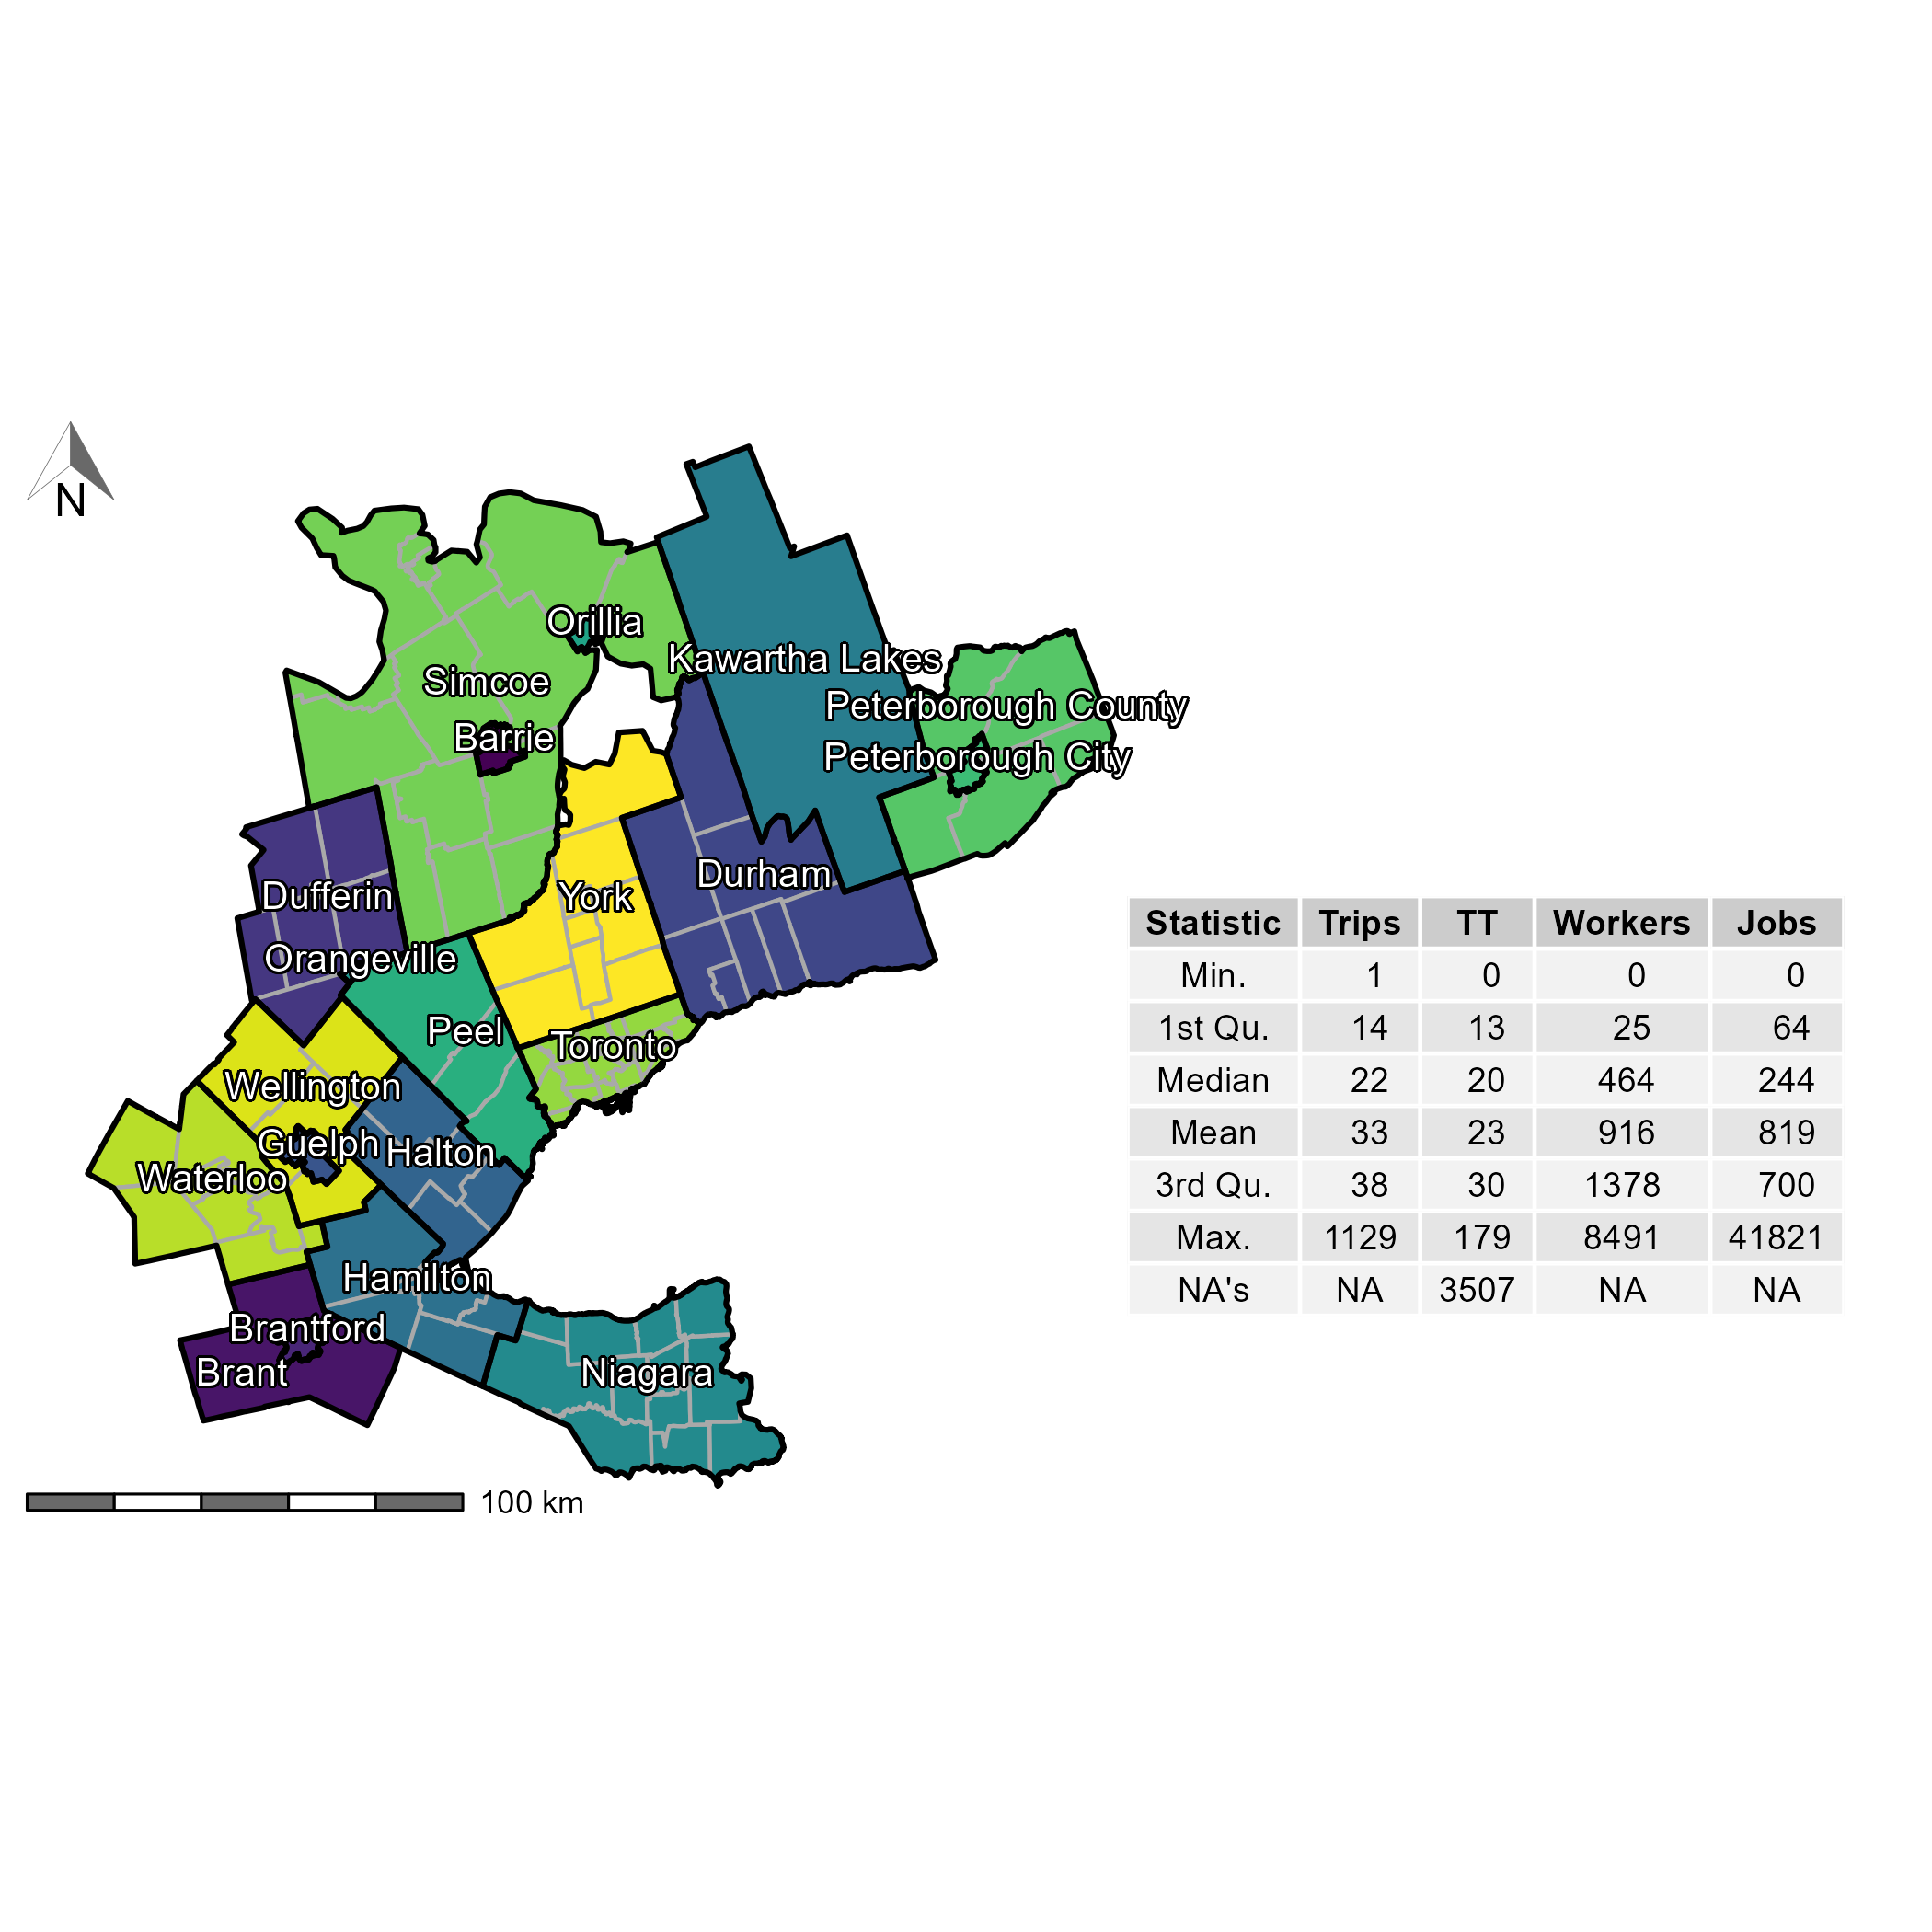
\includegraphics[width=1\linewidth]{images/TTS16-survey-area} 

}

\caption{\label{fig:TTS-16-survey-area}TTS 2016 study area (GGH, Ontario, Canada) along with the descriptive statistics of the trips, calculated origin-destination car travel time (TT), workers per TAZ, and jobs per TAZ. Contains 20 regions (black boundaries) and sub-regions (dark gray boundaries).}\label{fig:TTS-16-survey-area}
\end{figure}

\hypertarget{spatial-employment-characteristics-in-toronto}{%
\subsection{Spatial employment characteristics in
Toronto}\label{spatial-employment-characteristics-in-toronto}}

\begin{figure}
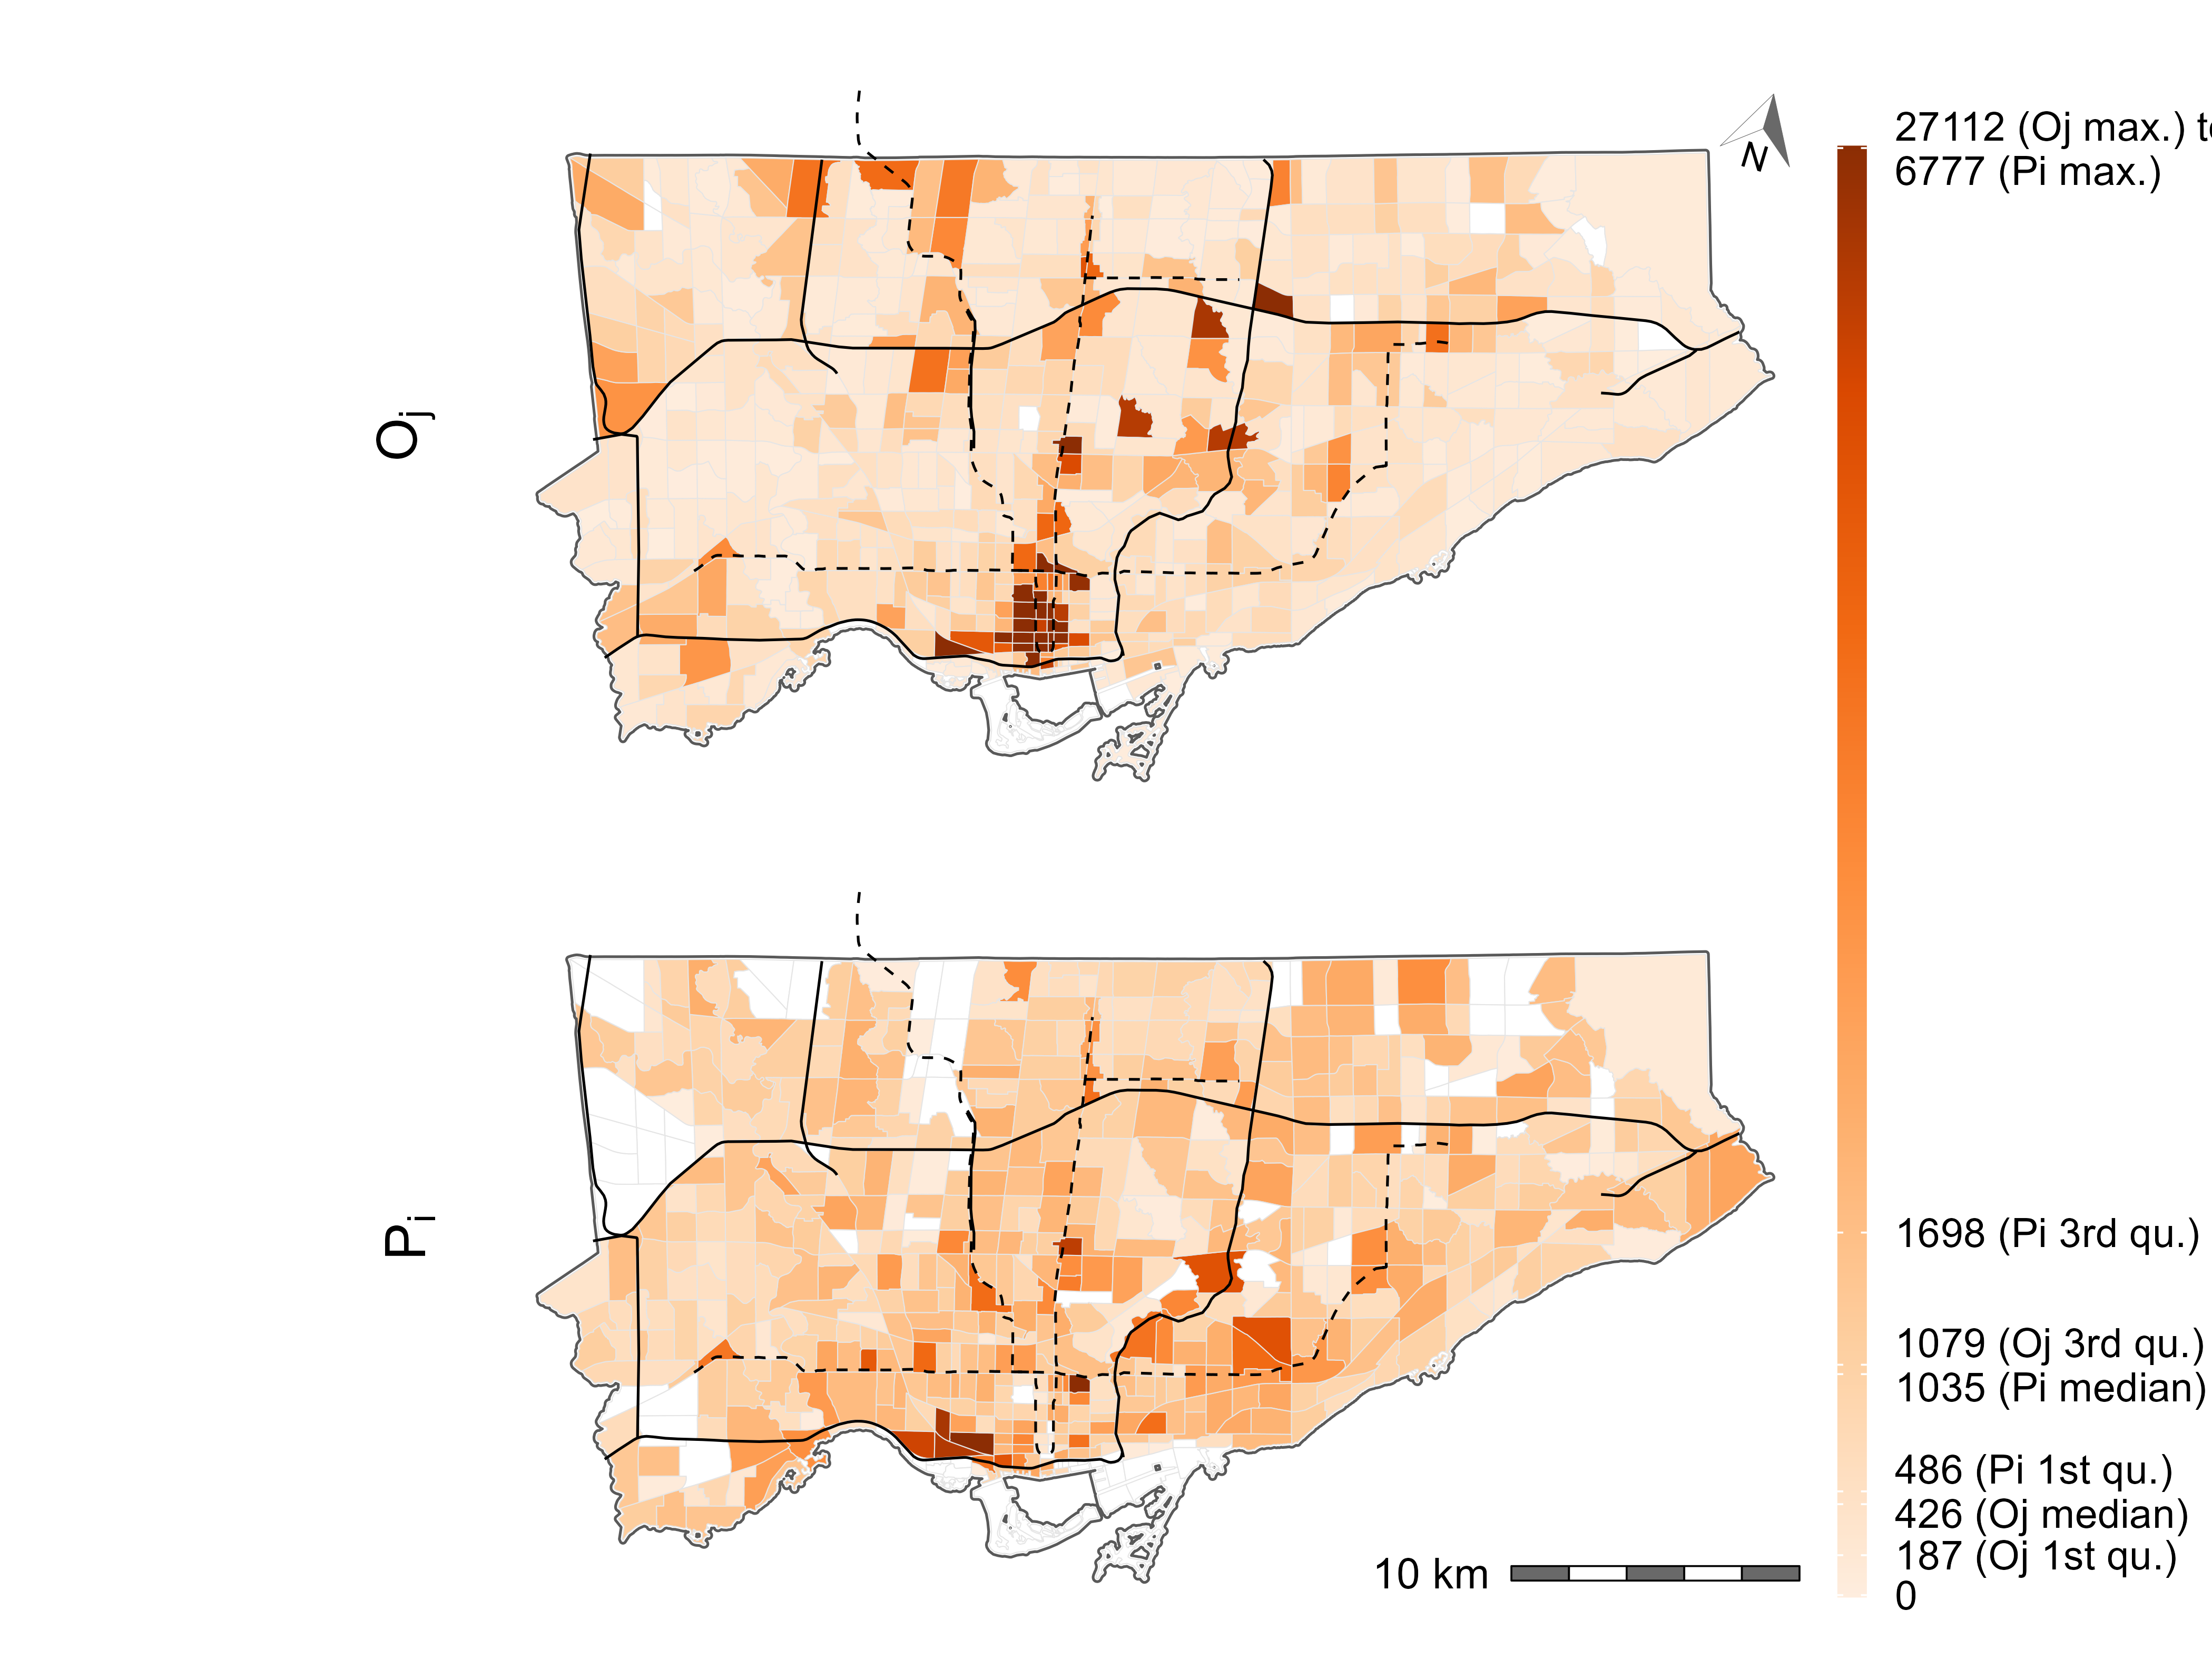
\includegraphics[width=1\linewidth]{images/spatial-dist-jobs-pop-Toronto-plot} \caption{\label{fig:s-dist-Toronto-plot}  Spatial distribution of full-time jobs (top) and full-time working population (bottom) for the city of Toronto as provided by the 2016 TTS. Black lines represent expressways and black dashed lines represent subway lines.}\label{fig:spatial-dist-Toronto-plot}
\end{figure}

\begin{figure}
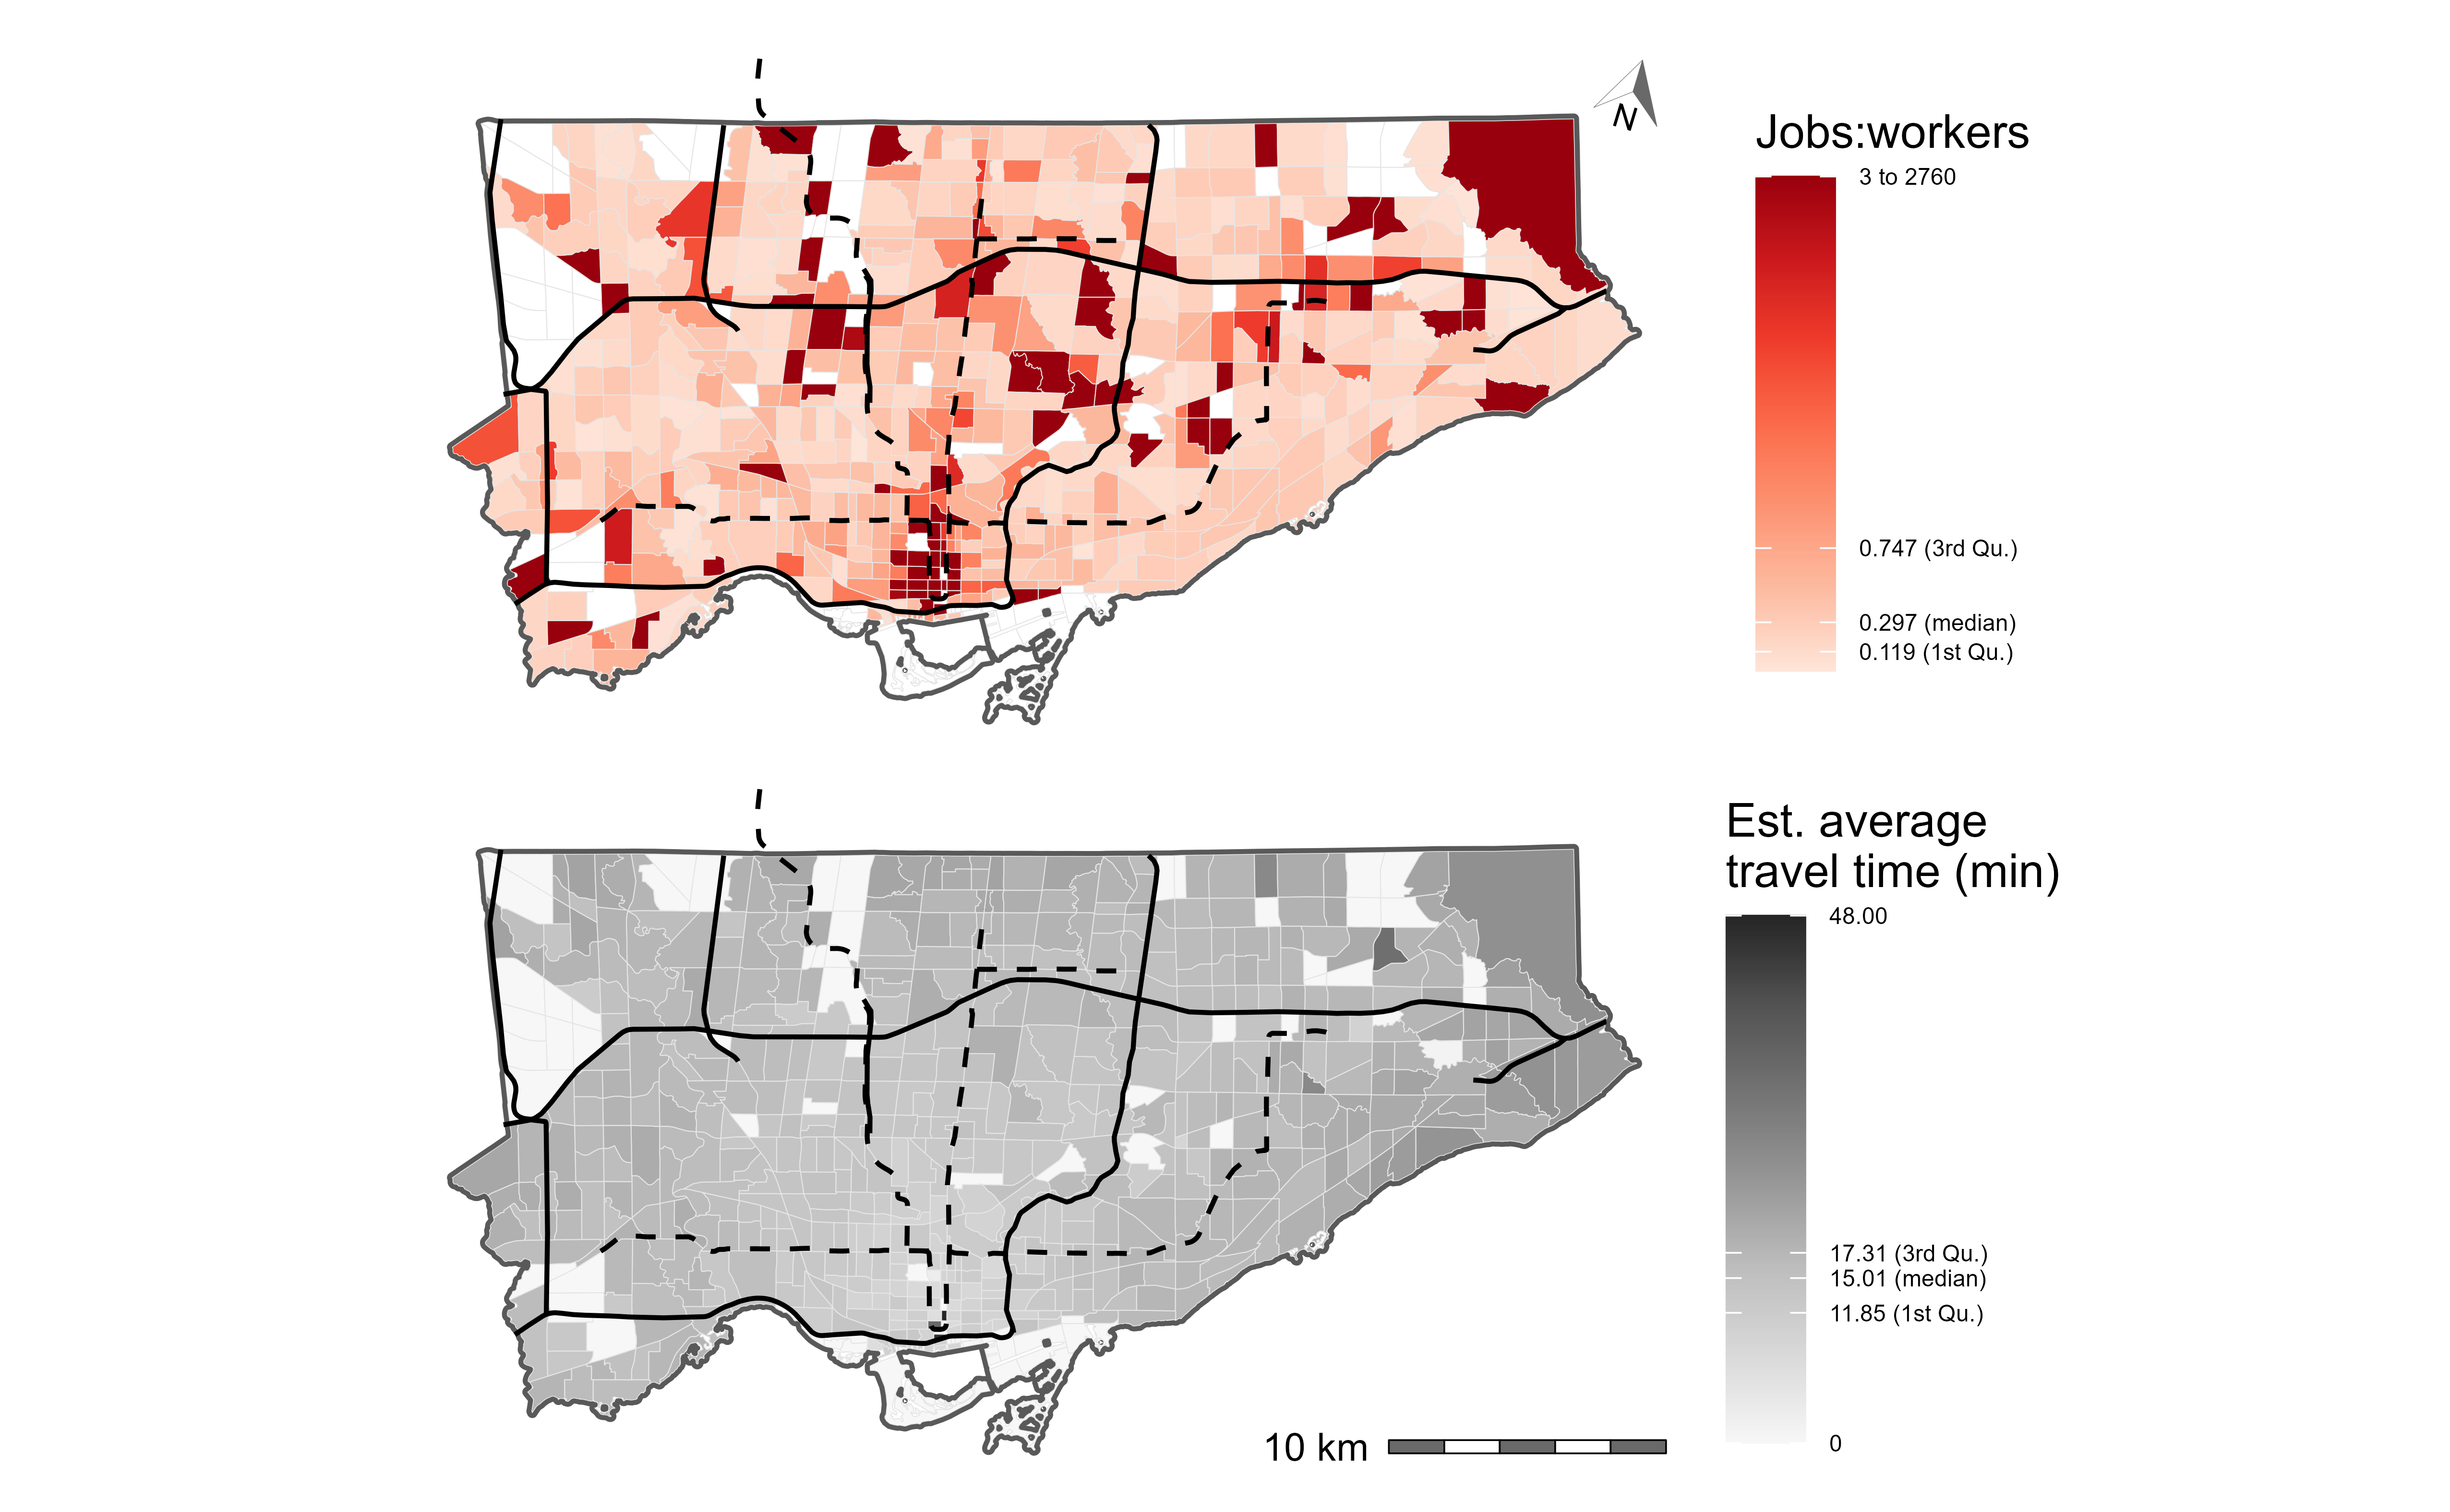
\includegraphics[width=1\linewidth]{images/spatial-dist-jobs-pop-Toronto-plot2} \caption{\label{fig:s-dist-Toronto-plot2}  Spatial distribution of full-time working jobs and worker ratio (top) and car travel time to jobs estimated using R5R for the city of Toronto as provided by the 2016 TTS. Black lines represent expressways and black dashed lines represent subway lines.}\label{fig:spatial-dist-Toronto-plot2}
\end{figure}

As mentioned, the focus of this empirical example is on the city of
Toronto. It is the largest city in the GGH and represents a significant
subset of workers and jobs in the GGH; 22\% of workers in the GGH live
in Toronto and 25\% of jobs that these workers take are located within
Toronto. The spatial distribution of jobs (purple) and workers (orange)
is shown in Figure \ref{fig:s-dist-Toronto-plot}. It can be seen that a
large cluster of jobs can be found in the central southern part of
Toronto (the downtown core). Spatial trends in the distribution of
workers is less apparent relative to the distribution of jobs.

Next, the spatial distribution of the jobs to workers ratio
(jobs:workers) (red) and the estimated car travel time (grey) is
visualized in Figure \ref{fig:s-dist-Toronto-plot2}. Some of the
jobs:workers balance predictably clusters near major transportation
networks (i.e, the north-south subway line and highways) where
surrounding land is more commonly zoned for commercial use. By contrast,
the estimated average travel time to work is more even throughout the
city, with lower travel times within the downtown core and longer travel
times for TAZ located further and further from the core. Interestingly,
travel times in certain TAZ with a high jobs:worker balance occur.

Nonetheless, the point of these visualizations is to demonstrate the
spatial distribution of worker and job data in the city of Toronto to
contextualize spatial availability and Shen- and Hansen- type measures.

\hypertarget{calibration-of-an-impedance-function-for-toronto}{%
\subsection{Calibration of an impedance function for
Toronto}\label{calibration-of-an-impedance-function-for-toronto}}

In the synthetic example introduced before, we used a negative
exponential function with the parameter reported by \citet{shen1998}.
For the empirical Toronto data set, we calibrate an impedance function
on the trip length distribution (TLD) of commute trips. Briefly, a TLD
represents the proportion of trips that are taken at a specific travel
cost (e.g., travel time); this distribution is commonly used to derive
impedance functions in accessibility research
\citep{lopez_2017_spatial, horbachov_theoretical_2018, batista_estimation_2019}.

As mentioned, the calculations are undertaken for the city of Toronto
using only the employed population in the city and jobs taken by
residents of Toronto. Specifically, edge trips are not included such as
trips originating in Toronto but finishing outside of Toronto and trips
originating outside of Toronto but finishing in Toronto. The empirical
and theoretical TLD for this Toronto data set are represented in the
top-left panel of Figure \ref{fig:TLD-norm-plot}. Maximum likelihood
estimation and the Nelder-Mead method for direct optimization available
within the \{fitdistrplus\} package \citep{fitdistrplus_2015} were used.
Based on goodness-of-fit criteria and diagnostics the normal
distribution was selected (see Figure \ref{fig:TLD-norm-plot}).

\begin{figure}

{\centering 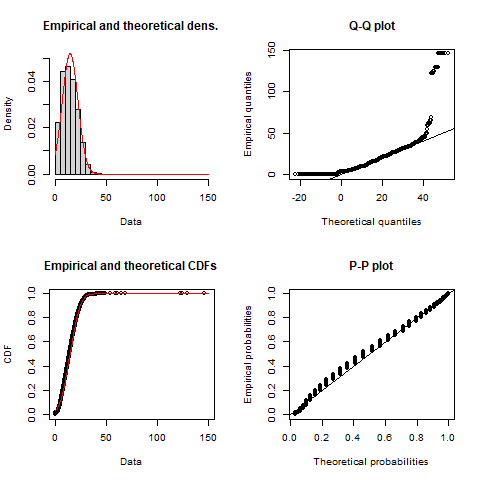
\includegraphics[width=0.8\linewidth]{images/impedance_function} 

}

\caption{\label{fig:TLD-norm-plot}Car trip length distribution and calibrated normal distribution impedance function (red line) with associated Q-Q and P-P plots. Based on TTS 2016.}\label{fig:TLD-norm-plot}
\end{figure}

The normal distribution is defined in Equation (\ref{norm-dist}), where
we see that it depends on a mean parameter \(\mu\) and a standard
deviation parameter \(\sigma\). The estimated values of these parameters
are \(\mu=\) 14.707 and \(\sigma =\) 7.697.

\begin{equation}
\label{norm-dist}
\begin{array}{l} 
f(x) = \frac{1}{\sigma \sqrt{2\pi}}e^{-\frac{1}{2}(\frac{x-\mu}{\sigma})^2}\\
\end{array}
\end{equation}

\[
\frac{1}{\sigma \sqrt{2\pi}}e^{\frac{1}{2}(\frac{x-\mu}{\sigma})^2}
\]

\hypertarget{accessibility-and-spatial-availability-of-jobs-in-toronto}{%
\subsection{Accessibility and spatial availability of jobs in
Toronto}\label{accessibility-and-spatial-availability-of-jobs-in-toronto}}

 
  \providecommand{\huxb}[2]{\arrayrulecolor[RGB]{#1}\global\arrayrulewidth=#2pt}
  \providecommand{\huxvb}[2]{\color[RGB]{#1}\vrule width #2pt}
  \providecommand{\huxtpad}[1]{\rule{0pt}{#1}}
  \providecommand{\huxbpad}[1]{\rule[-#1]{0pt}{#1}}

\begin{table}[ht]
\begin{centerbox}
\begin{threeparttable}
 \label{tab:verify-employment}
\setlength{\tabcolsep}{0pt}
\begin{tabular}{l}


\hhline{>{\huxb{0, 0, 0}{0.4}}-}
\arrayrulecolor{black}

\multicolumn{1}{!{\huxvb{0, 0, 0}{0.4}}r!{\huxvb{0, 0, 0}{0.4}}}{\huxtpad{6pt + 1em}\raggedleft \hspace{6pt} \textbf{jobs} \hspace{6pt}\huxbpad{6pt}} \tabularnewline[-0.5pt]


\hhline{>{\huxb{0, 0, 0}{0.4}}-}
\arrayrulecolor{black}

\multicolumn{1}{!{\huxvb{0, 0, 0}{0.4}}r!{\huxvb{0, 0, 0}{0.4}}}{\cellcolor[RGB]{242, 242, 242}\huxtpad{6pt + 1em}\raggedleft \hspace{6pt} 7.69e+05 \hspace{6pt}\huxbpad{6pt}} \tabularnewline[-0.5pt]


\hhline{>{\huxb{0, 0, 0}{0.4}}-}
\arrayrulecolor{black}
\end{tabular}
\end{threeparttable}\par\end{centerbox}

\end{table}
 

 
  \providecommand{\huxb}[2]{\arrayrulecolor[RGB]{#1}\global\arrayrulewidth=#2pt}
  \providecommand{\huxvb}[2]{\color[RGB]{#1}\vrule width #2pt}
  \providecommand{\huxtpad}[1]{\rule{0pt}{#1}}
  \providecommand{\huxbpad}[1]{\rule[-#1]{0pt}{#1}}

\begin{table}[ht]
\begin{centerbox}
\begin{threeparttable}
 \label{tab:verify-employment}
\setlength{\tabcolsep}{0pt}
\begin{tabular}{l}


\hhline{>{\huxb{0, 0, 0}{0.4}}-}
\arrayrulecolor{black}

\multicolumn{1}{!{\huxvb{0, 0, 0}{0.4}}r!{\huxvb{0, 0, 0}{0.4}}}{\huxtpad{6pt + 1em}\raggedleft \hspace{6pt} \textbf{jobs} \hspace{6pt}\huxbpad{6pt}} \tabularnewline[-0.5pt]


\hhline{>{\huxb{0, 0, 0}{0.4}}-}
\arrayrulecolor{black}

\multicolumn{1}{!{\huxvb{0, 0, 0}{0.4}}r!{\huxvb{0, 0, 0}{0.4}}}{\cellcolor[RGB]{242, 242, 242}\huxtpad{6pt + 1em}\raggedleft \hspace{6pt} 7.69e+05 \hspace{6pt}\huxbpad{6pt}} \tabularnewline[-0.5pt]


\hhline{>{\huxb{0, 0, 0}{0.4}}-}
\arrayrulecolor{black}
\end{tabular}
\end{threeparttable}\par\end{centerbox}

\end{table}
 

 
  \providecommand{\huxb}[2]{\arrayrulecolor[RGB]{#1}\global\arrayrulewidth=#2pt}
  \providecommand{\huxvb}[2]{\color[RGB]{#1}\vrule width #2pt}
  \providecommand{\huxtpad}[1]{\rule{0pt}{#1}}
  \providecommand{\huxbpad}[1]{\rule[-#1]{0pt}{#1}}

\begin{table}[ht]
\begin{centerbox}
\begin{threeparttable}
 \label{tab:verify-population}
\setlength{\tabcolsep}{0pt}
\begin{tabular}{l}


\hhline{>{\huxb{0, 0, 0}{0.4}}-}
\arrayrulecolor{black}

\multicolumn{1}{!{\huxvb{0, 0, 0}{0.4}}r!{\huxvb{0, 0, 0}{0.4}}}{\huxtpad{6pt + 1em}\raggedleft \hspace{6pt} \textbf{workers} \hspace{6pt}\huxbpad{6pt}} \tabularnewline[-0.5pt]


\hhline{>{\huxb{0, 0, 0}{0.4}}-}
\arrayrulecolor{black}

\multicolumn{1}{!{\huxvb{0, 0, 0}{0.4}}r!{\huxvb{0, 0, 0}{0.4}}}{\cellcolor[RGB]{242, 242, 242}\huxtpad{6pt + 1em}\raggedleft \hspace{6pt} 7.69e+05 \hspace{6pt}\huxbpad{6pt}} \tabularnewline[-0.5pt]


\hhline{>{\huxb{0, 0, 0}{0.4}}-}
\arrayrulecolor{black}
\end{tabular}
\end{threeparttable}\par\end{centerbox}

\end{table}
 

 
  \providecommand{\huxb}[2]{\arrayrulecolor[RGB]{#1}\global\arrayrulewidth=#2pt}
  \providecommand{\huxvb}[2]{\color[RGB]{#1}\vrule width #2pt}
  \providecommand{\huxtpad}[1]{\rule{0pt}{#1}}
  \providecommand{\huxbpad}[1]{\rule[-#1]{0pt}{#1}}

\begin{table}[ht]
\begin{centerbox}
\begin{threeparttable}
 \label{tab:verify-population}
\setlength{\tabcolsep}{0pt}
\begin{tabular}{l}


\hhline{>{\huxb{0, 0, 0}{0.4}}-}
\arrayrulecolor{black}

\multicolumn{1}{!{\huxvb{0, 0, 0}{0.4}}r!{\huxvb{0, 0, 0}{0.4}}}{\huxtpad{6pt + 1em}\raggedleft \hspace{6pt} \textbf{workers} \hspace{6pt}\huxbpad{6pt}} \tabularnewline[-0.5pt]


\hhline{>{\huxb{0, 0, 0}{0.4}}-}
\arrayrulecolor{black}

\multicolumn{1}{!{\huxvb{0, 0, 0}{0.4}}r!{\huxvb{0, 0, 0}{0.4}}}{\cellcolor[RGB]{242, 242, 242}\huxtpad{6pt + 1em}\raggedleft \hspace{6pt} 1.73e+06 \hspace{6pt}\huxbpad{6pt}} \tabularnewline[-0.5pt]


\hhline{>{\huxb{0, 0, 0}{0.4}}-}
\arrayrulecolor{black}
\end{tabular}
\end{threeparttable}\par\end{centerbox}

\end{table}
 

 
  \providecommand{\huxb}[2]{\arrayrulecolor[RGB]{#1}\global\arrayrulewidth=#2pt}
  \providecommand{\huxvb}[2]{\color[RGB]{#1}\vrule width #2pt}
  \providecommand{\huxtpad}[1]{\rule{0pt}{#1}}
  \providecommand{\huxbpad}[1]{\rule[-#1]{0pt}{#1}}

\begin{table}[ht]
\begin{centerbox}
\begin{threeparttable}
 \label{tab:verify-population}
\setlength{\tabcolsep}{0pt}
\begin{tabular}{l}


\hhline{>{\huxb{0, 0, 0}{0.4}}-}
\arrayrulecolor{black}

\multicolumn{1}{!{\huxvb{0, 0, 0}{0.4}}r!{\huxvb{0, 0, 0}{0.4}}}{\huxtpad{6pt + 1em}\raggedleft \hspace{6pt} \textbf{workers} \hspace{6pt}\huxbpad{6pt}} \tabularnewline[-0.5pt]


\hhline{>{\huxb{0, 0, 0}{0.4}}-}
\arrayrulecolor{black}

\multicolumn{1}{!{\huxvb{0, 0, 0}{0.4}}r!{\huxvb{0, 0, 0}{0.4}}}{\cellcolor[RGB]{242, 242, 242}\huxtpad{6pt + 1em}\raggedleft \hspace{6pt} 7.69e+05 \hspace{6pt}\huxbpad{6pt}} \tabularnewline[-0.5pt]


\hhline{>{\huxb{0, 0, 0}{0.4}}-}
\arrayrulecolor{black}
\end{tabular}
\end{threeparttable}\par\end{centerbox}

\end{table}
 

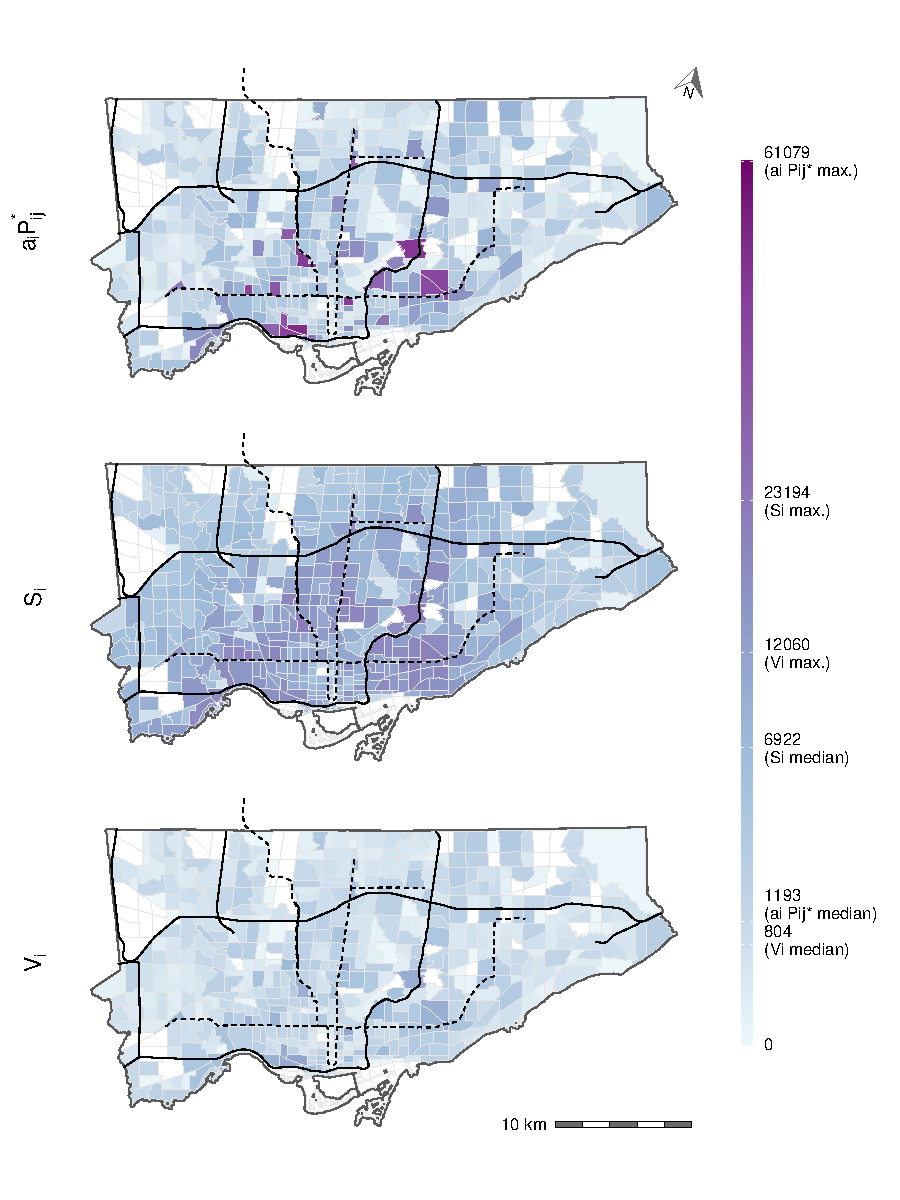
\includegraphics[width=1\linewidth]{Spatial-Availability-Refreshed_files/figure-latex/absolute-accessibility-plot-creation-1}

Figure \ref{fig:absolute-accessibility-plot} contains the absolute
accessibility values in number of jobs accessible using Shen-type
accessibility, Hansen-type accessibility, and the number of jobs
\emph{available} using the spatial availability measure. The Shen-type
accessibility is multiplied by the \emph{effective opportunity-seeking
population} to yield a value that corresponds to absolute number of
accessible jobs (considering competition) according to Shen's
definition. The Hansen-type accessibility is an unconstrained case of
accessibility in which all jobs which are in-reach of each origin
(according to the impedance function); each value corresponds to the
number of jobs which can be reach at each origin assuming no
competition. Lastly, the spatial availability measure is a constrained
case of accessibility which yields the number of jobs, at each origin,
considering competition from the population in nearby origin and the
relative travel cost (according to the impedance function).

The proportional allocation mechanism of spatial availability ensures
that the job availability value for each origin all sums to the
city-wide total of 769,231 jobs (i.e., the number of destination flows
from Toronto origins to Toronto destinations). The regional total for
Hansen-type accessibility is 4,318,005 jobs, which as a value is
meaningless since the measure is unconstrained; it represents the sum of
opportunities that have been counted anywhere from 1 to many times
depending on the impedance function. As previously discussed,
unconstrained counting of the same opportunity by all origins is not an
issue if the opportunity itself is non-exclusive, but since there is a
correspondence of one job and one worker, it is inappropriate to use
unconstrained measures to capture employment characteristics.

On a similar note to Hasen-type, the \emph{absolute} Shen-type measure
(as understood by Shen's definition of \(P_i\) being equal to
\(P_{ij}^*\) sums to the city-wide value of 2,064,055 jobs; this value
demonstrates how the Shen-type measure that is presented a rate (i.e.,
opportunities per capita) can be misunderstood and multiplied by the
\emph{effective opportunity-seeking population} (i.e., the denominator
of the rate \(P_{ij}^*\)) to express an absolute accessibility score.
Confounding \(P_i\) with \(P_{ij}^*\) yields an \emph{incorrect} number
of competitively accessible jobs because \(P_{ij}^*\) greatly exceeds
greatly exceeds the city-wide total of workers. To the authors'
knowledge, Shen-type accessibility has not been converted to the
absolute value in the way demonstrated within this paper. However, we
also have not seen the Shen-type measure converted from the
opportunities per capita score to absolute opportunities, we suspect,
because of the ambiguous definition which conflates \(P_{ij}^*\) with
\(P_i\). If \(a_i\) is multiplied by \(P_i\), it yields the same value
as \(V_i\), but, since the definition of Shen-type measure is equivocal
doing so is not clear since the denominator of \(a_i\) (which is a rate)
is \emph{not} \(P_i\).

 
  \providecommand{\huxb}[2]{\arrayrulecolor[RGB]{#1}\global\arrayrulewidth=#2pt}
  \providecommand{\huxvb}[2]{\color[RGB]{#1}\vrule width #2pt}
  \providecommand{\huxtpad}[1]{\rule{0pt}{#1}}
  \providecommand{\huxbpad}[1]{\rule[-#1]{0pt}{#1}}

\begin{table}[ht]
\begin{centerbox}
\begin{threeparttable}
 \label{tab:unnamed-chunk-3}
\setlength{\tabcolsep}{0pt}
\begin{tabular}{l l}


\hhline{>{\huxb{0, 0, 0}{0.4}}->{\huxb{0, 0, 0}{0.4}}-}
\arrayrulecolor{black}

\multicolumn{1}{!{\huxvb{0, 0, 0}{0.4}}r!{\huxvb{0, 0, 0}{0}}}{\huxtpad{6pt + 1em}\raggedleft \hspace{6pt} \textbf{osp} \hspace{6pt}\huxbpad{6pt}} &
\multicolumn{1}{r!{\huxvb{0, 0, 0}{0.4}}}{\huxtpad{6pt + 1em}\raggedleft \hspace{6pt} \textbf{total\_workers} \hspace{6pt}\huxbpad{6pt}} \tabularnewline[-0.5pt]


\hhline{>{\huxb{0, 0, 0}{0.4}}->{\huxb{0, 0, 0}{0.4}}-}
\arrayrulecolor{black}

\multicolumn{1}{!{\huxvb{0, 0, 0}{0.4}}r!{\huxvb{0, 0, 0}{0}}}{\cellcolor[RGB]{242, 242, 242}\huxtpad{6pt + 1em}\raggedleft \hspace{6pt} 1.73e+06 \hspace{6pt}\huxbpad{6pt}} &
\multicolumn{1}{r!{\huxvb{0, 0, 0}{0.4}}}{\cellcolor[RGB]{242, 242, 242}\huxtpad{6pt + 1em}\raggedleft \hspace{6pt} 7.69e+05 \hspace{6pt}\huxbpad{6pt}} \tabularnewline[-0.5pt]


\hhline{>{\huxb{0, 0, 0}{0.4}}->{\huxb{0, 0, 0}{0.4}}-}
\arrayrulecolor{black}
\end{tabular}
\end{threeparttable}\par\end{centerbox}

\end{table}
 

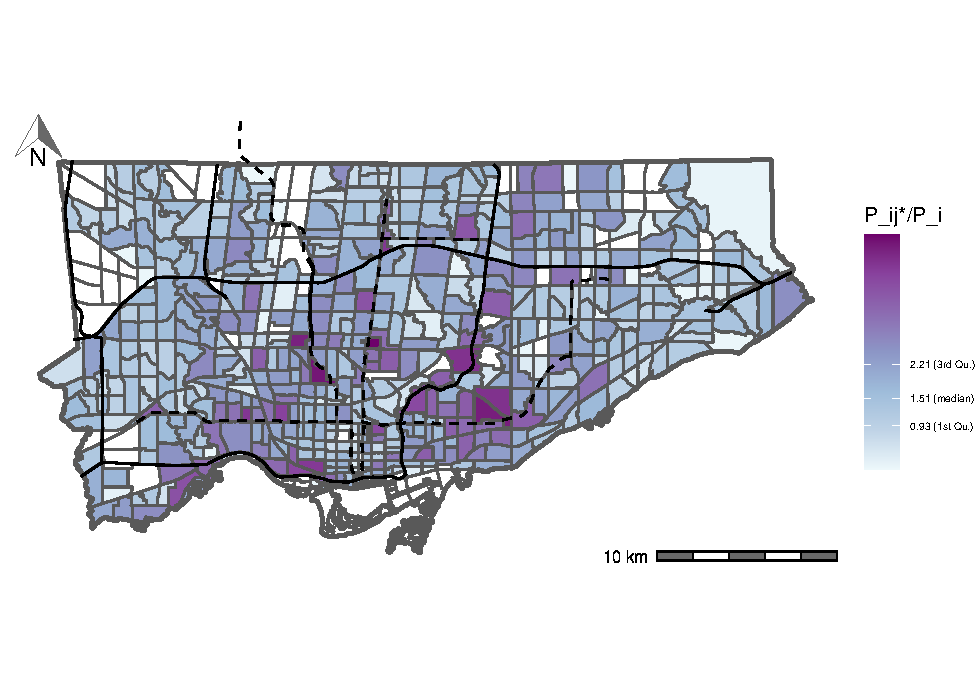
\includegraphics[width=1\linewidth]{Spatial-Availability-Refreshed_files/figure-latex/ratio-OPS-to-pop-plot-creation-1}

\begin{figure}
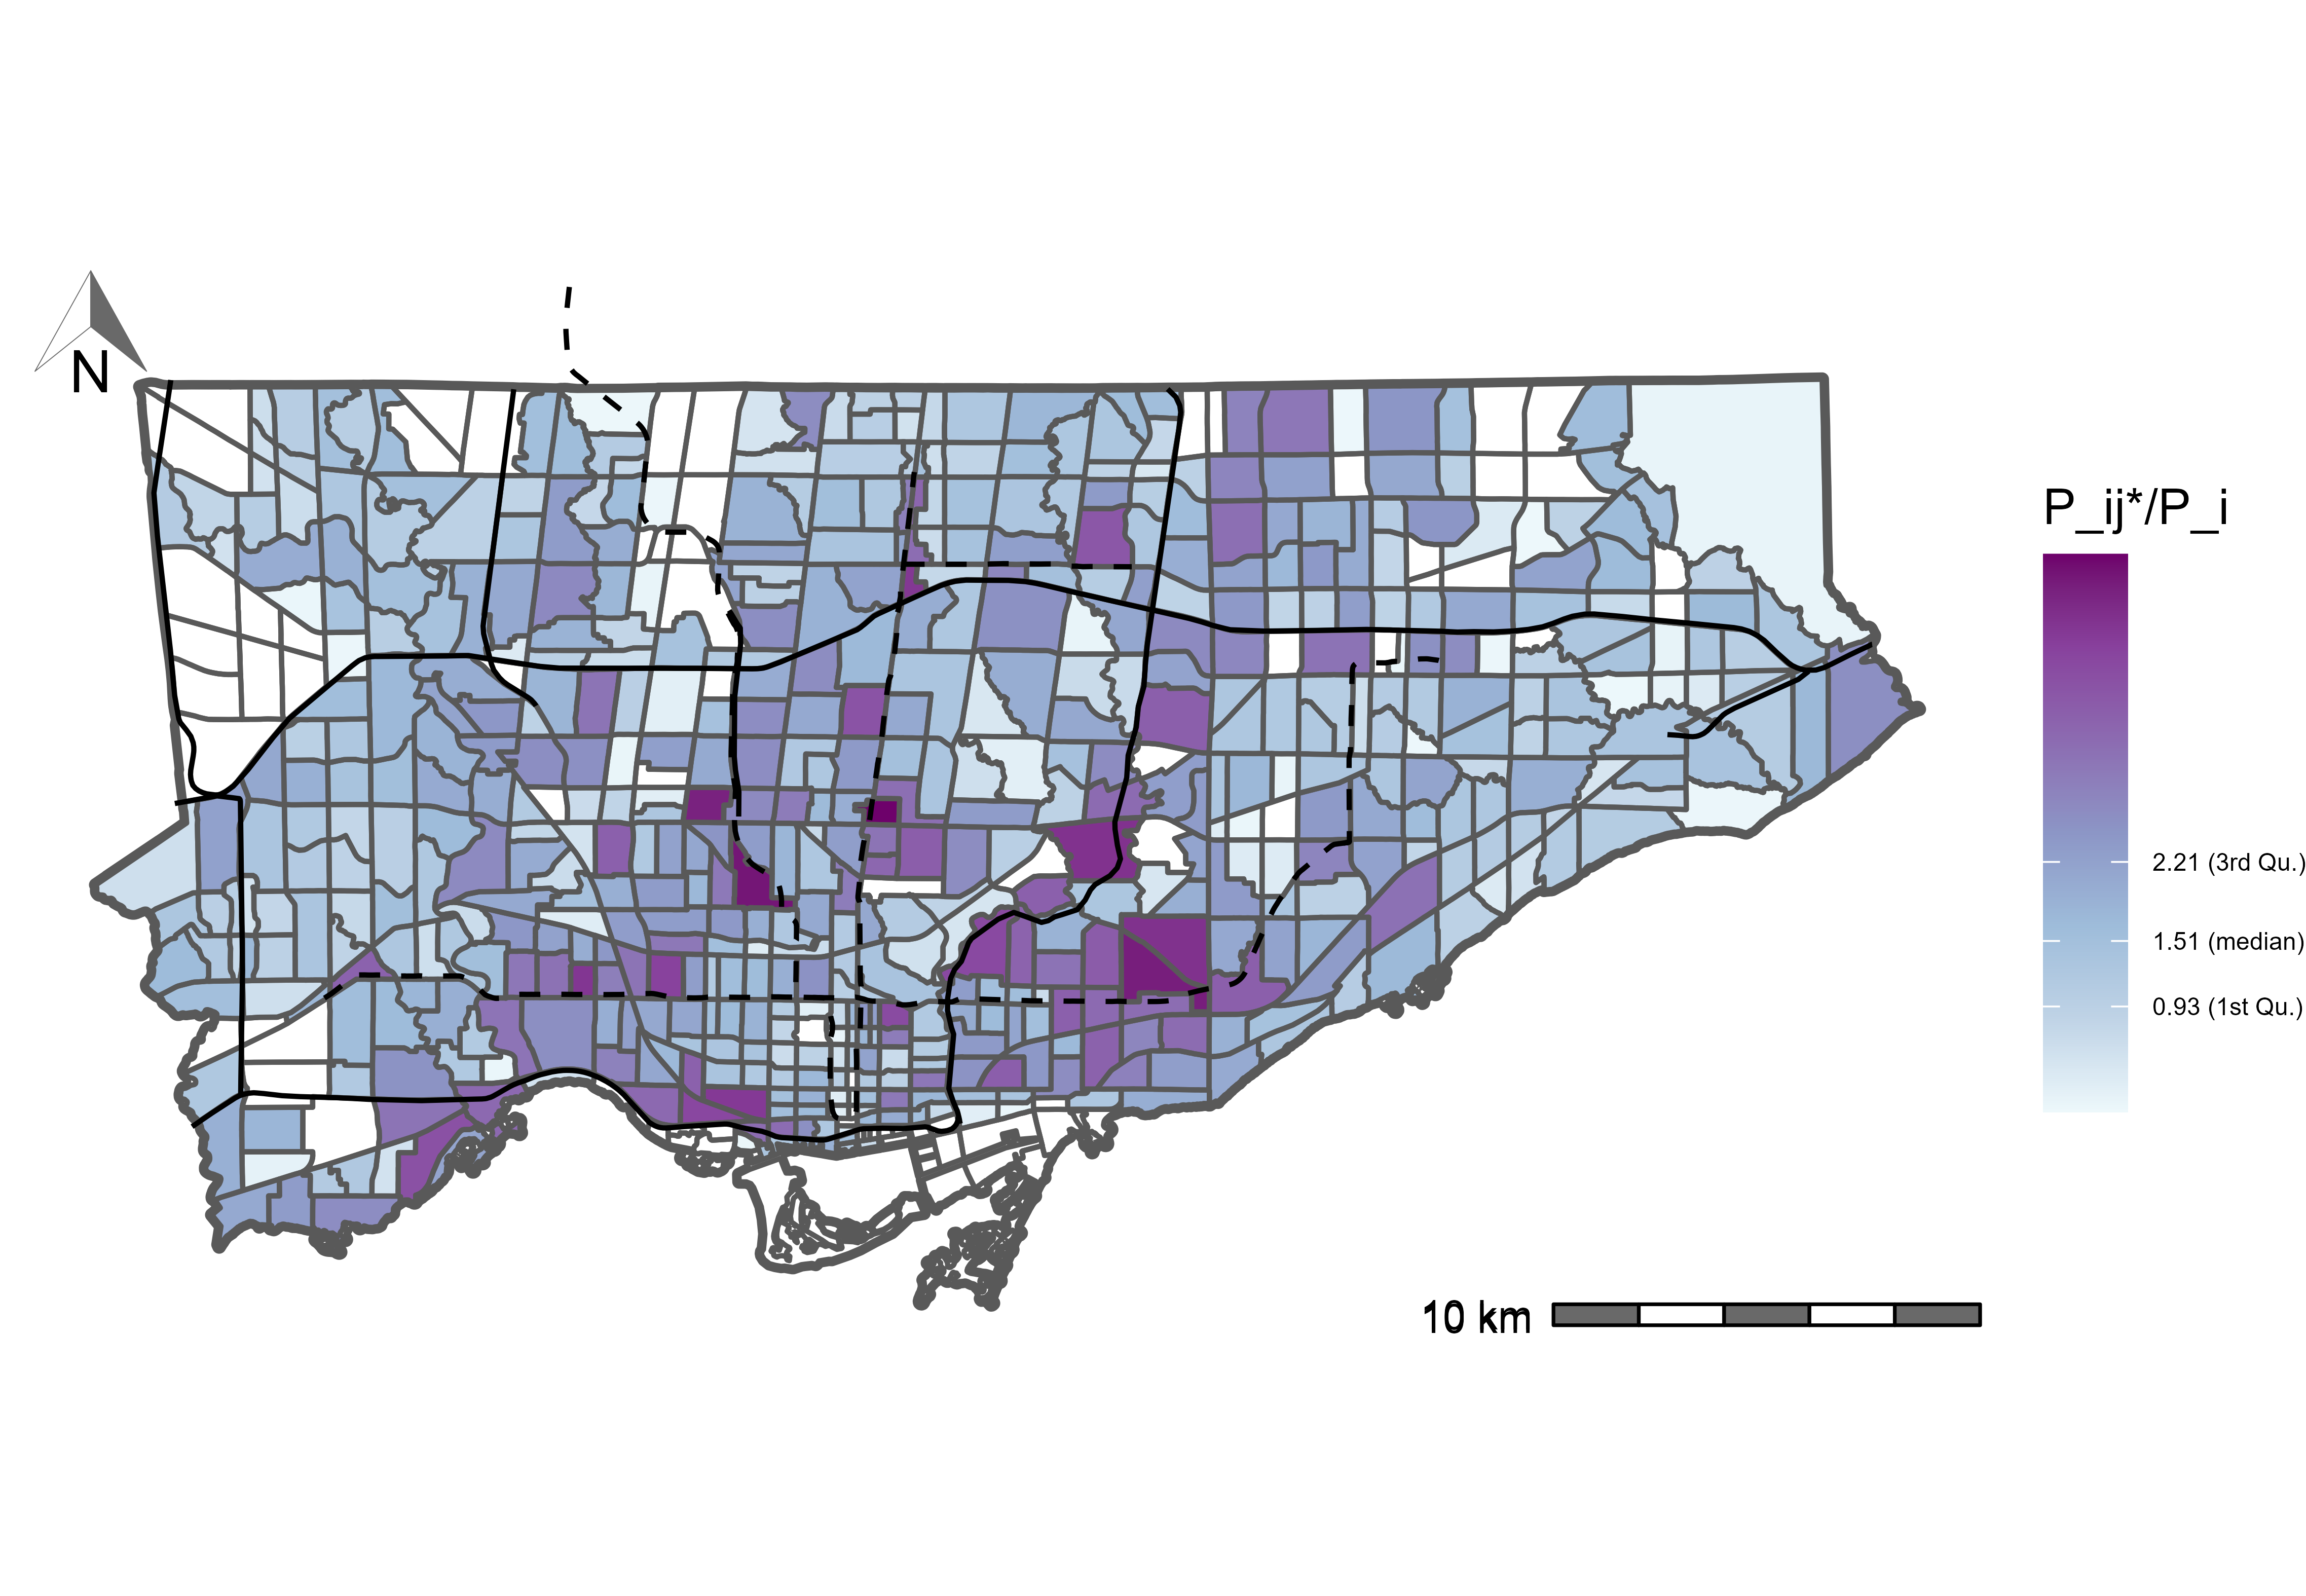
\includegraphics[width=1\linewidth]{images/osp_plot_TO} \caption{\label{fig:ratio-OPS-to-pop-plot}  The ratio of the effective opportunity seeking population to the population in Toronto. Black lines represent expressways and black dashed lines represent subway lines.}\label{fig:ratio-OPS-to-pop-plot}
\end{figure}

It is important to also highlight the differences between \(P_i\) and
\(P_{ij}^*\) since they are not uniform across space. Figure
\ref{fig:ratio-OPS-to-pop-plot} presents the ratio of \(P_{ij}^*\) to
\(P_i\) which shows how the effective opportunity-seeking population is
sometimes inflated and others deflated by \(a_i\). As a consequence of
the inflated population (i.e., \(P_{ij}^*\) \textgreater{} \(P_i\)), any
impacts of accessibility associated with the allocation of jobs to
workers by the Shen-type measure will be misleading. In the case of
city-wide travel time, we can see that travel time is exaggerated by the
Shen-type measure. Consequently, when using spatial availability and the
\emph{total} number of jobs in the city is preserved, travel time
calculations are more reliable.

 
  \providecommand{\huxb}[2]{\arrayrulecolor[RGB]{#1}\global\arrayrulewidth=#2pt}
  \providecommand{\huxvb}[2]{\color[RGB]{#1}\vrule width #2pt}
  \providecommand{\huxtpad}[1]{\rule{0pt}{#1}}
  \providecommand{\huxbpad}[1]{\rule[-#1]{0pt}{#1}}

\begin{table}[ht]
\begin{centerbox}
\begin{threeparttable}
 \label{tab:unnamed-chunk-4}
\setlength{\tabcolsep}{0pt}
\begin{tabular}{l}


\hhline{>{\huxb{0, 0, 0}{0.4}}-}
\arrayrulecolor{black}

\multicolumn{1}{!{\huxvb{0, 0, 0}{0.4}}l!{\huxvb{0, 0, 0}{0.4}}}{\huxtpad{6pt + 1em}\raggedright \hspace{6pt} \textbf{total\_travel\_time} \hspace{6pt}\huxbpad{6pt}} \tabularnewline[-0.5pt]


\hhline{>{\huxb{0, 0, 0}{0.4}}-}
\arrayrulecolor{black}

\multicolumn{1}{!{\huxvb{0, 0, 0}{0.4}}l!{\huxvb{0, 0, 0}{0.4}}}{\cellcolor[RGB]{242, 242, 242}\huxtpad{6pt + 1em}\raggedright \hspace{6pt} 497258.183377296 \hspace{6pt}\huxbpad{6pt}} \tabularnewline[-0.5pt]


\hhline{>{\huxb{0, 0, 0}{0.4}}-}
\arrayrulecolor{black}
\end{tabular}
\end{threeparttable}\par\end{centerbox}

\end{table}
 

 
  \providecommand{\huxb}[2]{\arrayrulecolor[RGB]{#1}\global\arrayrulewidth=#2pt}
  \providecommand{\huxvb}[2]{\color[RGB]{#1}\vrule width #2pt}
  \providecommand{\huxtpad}[1]{\rule{0pt}{#1}}
  \providecommand{\huxbpad}[1]{\rule[-#1]{0pt}{#1}}

\begin{table}[ht]
\begin{centerbox}
\begin{threeparttable}
 \label{tab:unnamed-chunk-4}
\setlength{\tabcolsep}{0pt}
\begin{tabular}{l}


\hhline{>{\huxb{0, 0, 0}{0.4}}-}
\arrayrulecolor{black}

\multicolumn{1}{!{\huxvb{0, 0, 0}{0.4}}l!{\huxvb{0, 0, 0}{0.4}}}{\huxtpad{6pt + 1em}\raggedright \hspace{6pt} \textbf{total\_travel\_time} \hspace{6pt}\huxbpad{6pt}} \tabularnewline[-0.5pt]


\hhline{>{\huxb{0, 0, 0}{0.4}}-}
\arrayrulecolor{black}

\multicolumn{1}{!{\huxvb{0, 0, 0}{0.4}}l!{\huxvb{0, 0, 0}{0.4}}}{\cellcolor[RGB]{242, 242, 242}\huxtpad{6pt + 1em}\raggedright \hspace{6pt} 187393.373611765 \hspace{6pt}\huxbpad{6pt}} \tabularnewline[-0.5pt]


\hhline{>{\huxb{0, 0, 0}{0.4}}-}
\arrayrulecolor{black}
\end{tabular}
\end{threeparttable}\par\end{centerbox}

\end{table}
 

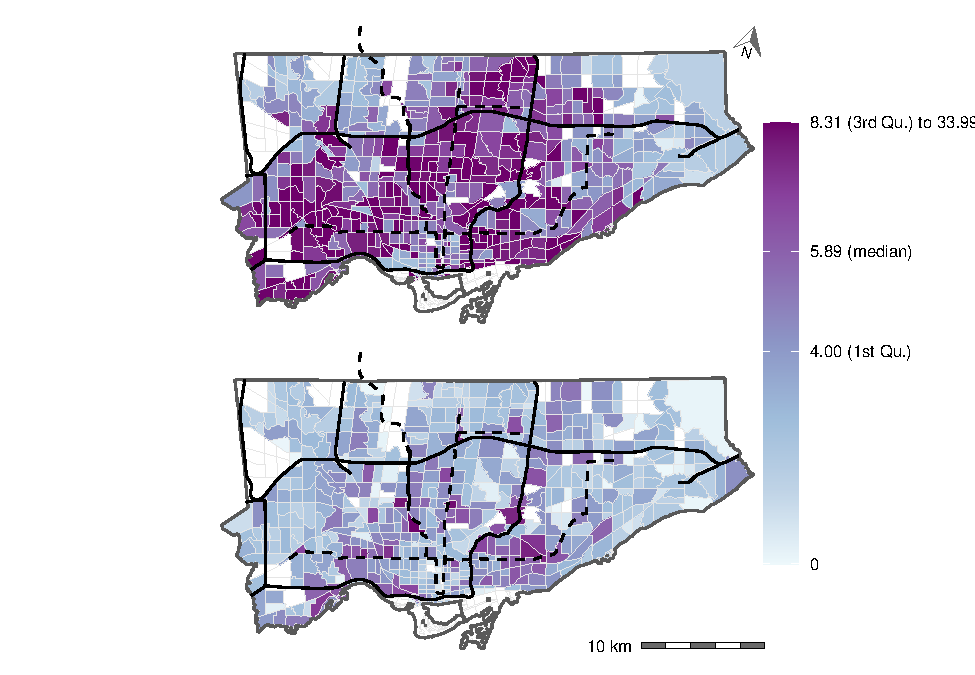
\includegraphics[width=1\linewidth]{Spatial-Availability-Refreshed_files/figure-latex/rate-accessibility-plot-creation-1}

Spatial availability untangles Shen-stype measure so an absolute value
of \emph{opportunity availability} is expressed. Because the
proportional allocation mechanism makes clear that all the opportunities
are being allocated proportionally to origins, it makes the
interpretation more clear. It thus can be directly divided by origin
population and expressed as an opportunities per capita score. This
score, while equal to the Shen-type measure, has a renewed
interpretability. When spatial availability is compared to Hansen-type
measure, normalizing the output by population directly is unique;
spatial availability can be normalized by opportunities without the
issue of multiple counting of opportunities which obscures
accessibility's meaning. See Figure \ref{fig:rate-accessibility-plot}
which displays the normalized opportunity per capita spatial
availability score and plainly normalizing Hansen-type accessibility by
dividing each value by the origin population.

\newpage

\hypertarget{conclusions}{%
\section{Conclusions}\label{conclusions}}

Why do differences between Hansen-style measure and the interpretation
of Shen-type measure matter? Because of equity analysis and policy
planning! With spatial availability, we can push accessibility analysis
forward by making it more interpretable. As discussed, Hansen-style
accessibility value cannot be interpreted directly in either form
(though it can be interpreted relatively to speak about urban form). By
contrast, spatial availability yields the number of jobs available
directly.

This property and understanding spatial availability (along with Shen's
accessibility with competition and 2SFCA) as a singly-constrained
measure are important to understanding how accessibility measures can be
broadled interepted. The following are recommendations:

\begin{enumerate}
\def\labelenumi{\arabic{enumi})}
\tightlist
\item
  The Hansen-style accessibilty should be used when opportunities are
  non-exclusive. When opportunities are perfectly exclusive (i.e., 1
  spot for 1 person), spatial availability (i.e., accessibility with
  competition) should be used.
\item
  Though outside of scope, when opportunities are perfectly exclusive ad
  -We argue that spatial availability should be used
\end{enumerate}

\begin{itemize}
\tightlist
\item
  some literature which uses Shen focuses on how travel cost discounts
  job supply (opportunities) and demand (opportunity-seeking
  population). This gets close to disentangling which population
  \emph{effectively} seeking opportunities - but comparing it to the
  population which doesn't seek opportunities has not been made, to the
  authors opportunity. This is critical for equity analysis; i.e., which
  populations can't seek opportunities because of friction of distance?
  This can be plainly seen by seeing the proportion of population, in
  spatial availability, which is allocated to the origin
\end{itemize}

\hypertarget{appendix-a}{%
\section{Appendix A}\label{appendix-a}}

Equivalence of Shen-type accessibility and spatial availability.

The population-based balancing factor used in \(V_i\) is defined as: \[
F^p_{ij} = \frac{P_{i\in r}^\alpha}{\sum_{i}^K P_{i\in r}^\alpha}
\]

\[
F^p_{A} = \frac{P_{A}^\alpha}{P_{A}^\alpha + P_{B}^\alpha + P_{C}^\alpha}
\]

The impedance-based balancing factor in \(V_i\) is:

\[
F^c_{ij} = \frac{f(c_{ij})}{\sum_{i=A}^K f(c_{ij})}
\]

\[
F^c_{A1} = \frac{f(c_{A1})}{f(c_{A1})+f(c_{B1})+f(c_{C1})}
\]

\[
F^c_{B1} = \frac{f(c_{A2})}{f(c_{A2})+f(c_{B2})+f(c_{C2})}
\]

\[
F^c_{C1} = \frac{f(c_{A3})}{f(c_{A3})+f(c_{B3})+f(c_{C3})}
\]

These factors when assembled together with \(P\) makes the denominators
cancel out:

\[
v_{i} = \sum_{j}\frac{O_j}{P_{i\in r}^\alpha}\frac{\frac{P_{i\in r}^\alpha}{\sum_{i}^K P_{i\in r}^\alpha} \cdot \frac{f(c_{ij})}{\sum_{i}^K f(c_{ij})}}{\sum_{i}^K \frac{P_{i\in r}^\alpha}{\sum_{i}^K P_{i\in r}^\alpha} \cdot \frac{f(c_{ij})}{\sum_{i}^K f(c_{ij})}}
\]

\[
v_{A} = \frac{O_1}{P_{A}^\alpha}(\frac{\frac{P_{A}^\alpha}{P_{A}^\alpha+P_{B}^\alpha+P_{C}^\alpha} \cdot \frac{f(c_{A1})}{f(c_{A1})+f(c_{B1})+f(c_{C1})}}{\frac{P_{A}^\alpha}{P_{A}^\alpha+P_{B}^\alpha+P_{C}^\alpha} \cdot \frac{f(c_{A1})}{f(c_{A1})+f(c_{B1})+f(c_{C1})} + \frac{P_{A}^\alpha}{P_{A}^\alpha+P_{B}^\alpha+P_{C}^\alpha} \cdot \frac{f(c_{B1})}{f(c_{A1})+f(c_{B1})+f(c_{C1})}+ \frac{P_{A}^\alpha}{P_{A}^\alpha+P_{B}^\alpha+P_{C}^\alpha} \cdot \frac{f(c_{C1})}{f(c_{A1})+f(c_{B1})+f(c_{C1})}}) +
\]

\[
\frac{O_2}{P_{A}^\alpha}(\frac{\frac{P_{A}^\alpha}{P_{A}^\alpha+P_{B}^\alpha+P_{C}^\alpha} \cdot \frac{f(c_{A2})}{f(c_{A2})+f(c_{B2})+f(c_{C2})}}{\frac{P_{A}^\alpha}{P_{A}^\alpha+P_{B}^\alpha+P_{C}^\alpha} \cdot \frac{f(c_{A2})}{f(c_{A2})+f(c_{B2})+f(c_{C2})} + \frac{P_{A}^\alpha}{P_{A}^\alpha+P_{B}^\alpha+P_{C}^\alpha} \cdot \frac{f(c_{B2})}{f(c_{A2})+f(c_{B2})+f(c_{C2})}+\frac{P_{A}^\alpha}{P_{A}^\alpha+P_{B}^\alpha+P_{C}^\alpha} \cdot \frac{f(c_{C2})}{f(c_{A2})+f(c_{B2})+f(c_{C2})}} )+
\]

\[
\frac{O_3}{P_{A}^\alpha}(\frac{\frac{P_{A}^\alpha}{P_{A}^\alpha+P_{B}^\alpha+P_{C}^\alpha} \cdot \frac{f(c_{A3})}{f(c_{A3})+f(c_{B3})+f(c_{C3})}}{\frac{P_{A}^\alpha}{P_{A}^\alpha+P_{B}^\alpha+P_{C}^\alpha} \cdot \frac{f(c_{A3})}{f(c_{A3})+f(c_{B3})+f(c_{C3})} + \frac{P_{A}^\alpha}{P_{A}^\alpha+P_{B}^\alpha+P_{C}^\alpha} \cdot \frac{f(c_{B3})}{f(c_{A3})+f(c_{B3})+f(c_{C3})}+\frac{P_{A}^\alpha}{P_{A}^\alpha+P_{B}^\alpha+P_{C}^\alpha} \cdot \frac{f(c_{C3})}{f(c_{A3})+f(c_{B3})+f(c_{C3})}} )
\]

First, notice how the denominator on the denominator is the same across
the summation. Simplifying:

\[
v_{A} = \frac{O_1}{P_{A}^\alpha}(\frac{\frac{P_{A}^\alpha}{P_{A}^\alpha+P_{B}^\alpha+P_{C}^\alpha} \cdot \frac{f(c_{A1})}{f(c_{A1})+f(c_{B1})+f(c_{C1})}}{\frac{P_{A}^\alpha \cdot f(c_{A1}) + P_{A}^\alpha \cdot f(c_{B1}) + P_{A}^\alpha \cdot f(c_{C1})}{(P_{A}^\alpha+P_{B}^\alpha+P_{C}^\alpha) \cdot (f(c_{A1})+f(c_{B1})+f(c_{C1}))}})
\]

\[\frac{O_2}{P_{A}^\alpha}(\frac{\frac{P_{A}^\alpha}{P_{A}^\alpha+P_{B}^\alpha+P_{C}^\alpha} \cdot \frac{f(c_{A2})}{f(c_{A2})+f(c_{B2})+f(c_{C2})}}{\frac{P_{A}^\alpha \cdot f(c_{A2}) + P_{A}^\alpha \cdot f(c_{B2}) + P_{A}^\alpha \cdot f(c_{C2})}{(P_{A}^\alpha+P_{B}^\alpha+P_{C}^\alpha) \cdot (f(c_{A2})+f(c_{B2})+f(c_{C2}))}})
\]

\[
\frac{O_3}{P_{A}^\alpha}(\frac{\frac{P_{A}^\alpha}{P_{A}^\alpha+P_{B}^\alpha+P_{C}^\alpha} \cdot \frac{f(c_{A3})}{f(c_{A3})+f(c_{B3})+f(c_{C3})}}{\frac{P_{A}^\alpha \cdot f(c_{A3}) + P_{A}^\alpha \cdot f(c_{B3}) + P_{A}^\alpha \cdot f(c_{C3})}{(P_{A}^\alpha+P_{B}^\alpha+P_{C}^\alpha) \cdot (f(c_{A3})+f(c_{B3})+f(c_{C3}))}} )
\]

Notice how the denominator of the denominator is the same as the
denominator of the numerator for each \(J\) (J=1, J=2, and J=3)? Cancel
those out and simplify:

\[
v_{A} = \frac{O_1}{P_{A}^\alpha}(\frac{P_{A}^\alpha \cdot f(c_{A1})}{P_{A}^\alpha \cdot f(c_{A1}) + P_{A}^\alpha \cdot f(c_{B1}) + P_{A}^\alpha \cdot f(c_{C1})}
\]

\[\frac{O_2}{P_{A}^\alpha}\frac{P_{A}^\alpha \cdot f(c_{A2})}{P_{A}^\alpha \cdot f(c_{A2}) + P_{A}^\alpha \cdot f(c_{B2}) + P_{A}^\alpha \cdot f(c_{C2})}
\]

\[
\frac{O_3}{P_{A}^\alpha}\frac{P_{A}^\alpha \cdot f(c_{A3})}{P_{A}^\alpha \cdot f(c_{A3}) + P_{A}^\alpha \cdot f(c_{B3}) + P_{A}^\alpha \cdot f(c_{C3})} )
\]

Next, we can cancel out the \(P_{A}^\alpha\):

\[
v_{A} = O_1(\frac{f(c_{A1})}{P_{A}^\alpha \cdot f(c_{A1}) + P_{B}^\alpha \cdot f(c_{B1}) + P_{C}^\alpha \cdot f(c_{C1})} + O_2\frac{f(c_{A2})}{P_{A}^\alpha \cdot f(c_{A2}) + P_{B}^\alpha \cdot f(c_{B2}) + P_{C}^\alpha \cdot f(c_{C2})} + O_3\frac{f(c_{A3})}{P_{A}^\alpha \cdot f(c_{A3}) + P_{B}^\alpha \cdot f(c_{B3}) + P_{C}^\alpha \cdot f(c_{C3})} )
\] \noindent which shows how \(v_A\) if formally indentical to the
Shen-type accessibility measure with competition.

\newpage

\renewcommand\refname{References}
\bibliography{bibliography.bib}


\end{document}
